\documentclass[a4paper]{scrartcl}

\usepackage[
fancytheorems,
fancyproofs,
noindent
]{adam}

\usepackage{tikz}
\usepackage{physics}
\usetikzlibrary{decorations.pathreplacing}

\title{Quantum Information and Computation}
\author{Adam Kelly (\texttt{ak2316@cam.ac.uk})}
\date{\today}

\allowdisplaybreaks

% ---------------------------------------------------------------------------
%  Extra macros
% ---------------------------------------------------------------------------

\newcommand{\class}[1]{\mathsf{#1}}
\newcommand{\QFT}{\operatorname{QFT}}
\DeclareMathOperator{\poly}{poly}
\newcommand{\Vs}{\mathcal{V}}
\newcommand{\Ws}{\mathcal{W}}
\newcommand{\Es}{\mathcal{E}}
\newcommand{\Ss}{\mathcal{S}}
\newcommand{\Bs}{\mathcal{B}}
\newcommand{\Ps}{\mathcal{P}}
\newcommand{\CX}{\mathrm{CX}}
\newcommand{\CZ}{\mathrm{CZ}}
\newcommand{\bits}[1]{\mathbb{B}_{#1}}
\newcommand{\CP}{\mathbb{CP}}

\declaretheorem[style=thmdefinitionbox,name=Method,sibling=theorem]{method}
\declaretheorem[style=thmdefinitionbox,name=Method,numbered=no]{method*}

% ---------------------------------------------------------------------------
%  A small home-made library for drawing quantum circuits in plain TikZ.
%  Coordinates are (column, -row): wires run left to right, rows go downwards.
%  Draw order in each picture: wires, then vertical links, then gates, then dots.
% ---------------------------------------------------------------------------

\tikzset{
  qw/.style={line width=0.5pt},
  qgt/.style={draw, line width=0.5pt, fill=white, rounded corners=0.5pt,
              minimum width=6.5mm, minimum height=6.5mm, inner sep=1.5pt, font=\small},
  qcd/.style={circle, fill=black, minimum size=1.6mm, inner sep=0pt}
}
\newcommand{\qcircuit}[1]{\begin{tikzpicture}[x=1.05cm,y=0.85cm,baseline]#1\end{tikzpicture}}
\newcommand{\qwire}[3]{\draw[qw] (#2,#1) -- (#3,#1);}
\newcommand{\qcwire}[3]{\draw[qw,double,double distance=1.1pt] (#2,#1) -- (#3,#1);}
\newcommand{\qlink}[3]{\draw[qw] (#1,#2) -- (#1,#3);}
\newcommand{\qclink}[3]{\draw[qw,double,double distance=1.1pt] (#1,#2) -- (#1,#3);}
\newcommand{\qg}[3]{\node[qgt] at (#1,#2) {$#3$};}
\newcommand{\qgb}[4]{\node[qgt,minimum width=#4] at (#1,#2) {$#3$};}
\newcommand{\qdot}[2]{\node[qcd] at (#1,#2) {};}
\newcommand{\qopen}[2]{\draw[qw,fill=white] (#1,#2) circle[radius=1.1mm];}
\newcommand{\qtarg}[2]{%
  \draw[qw,fill=white] (#1,#2) circle[radius=2.1mm];
  \draw[qw] (#1,#2) ++(-2.1mm,0) -- ++(4.2mm,0);
  \draw[qw] (#1,#2) ++(0,-2.1mm) -- ++(0,4.2mm);}
\newcommand{\qcross}[2]{%
  \draw[qw] (#1,#2) ++(-1.5mm,-1.5mm) -- ++(3mm,3mm);
  \draw[qw] (#1,#2) ++(-1.5mm,1.5mm) -- ++(3mm,-3mm);}
\newcommand{\qmeter}[2]{%
  \node[qgt,minimum width=7.5mm] at (#1,#2) {};
  \draw[qw] (#1,#2) ++(-2.2mm,-1.3mm) arc[start angle=180,end angle=0,radius=2.2mm];
  \draw[qw] (#1,#2) ++(0,-1.3mm) -- ++(1.7mm,2.9mm);}
\newcommand{\qlab}[3]{\node[left,inner sep=3pt,font=\small] at (#1,#2) {$#3$};}
\newcommand{\qrlab}[3]{\node[right,inner sep=3pt,font=\small] at (#1,#2) {$#3$};}
\newcommand{\qtext}[3]{\node[font=\small] at (#1,#2) {#3};}
\newcommand{\qbig}[5]{%
  \filldraw[qw,fill=white,rounded corners=0.5pt] (#1-#4,#2+0.32) rectangle (#1+#4,#3-0.32);
  \node[font=\small] at (#1,{(#2+#3)/2}) {$#5$};}

\begin{document}

\maketitle

A computer is a physical object, and a computation is something that a physical object does. That sounds like a platitude, but it has teeth: whatever we can and cannot compute is decided not by mathematics alone but by the laws of physics that the computer happens to obey. For most of the twentieth century the physics we implicitly assumed was classical, and the resulting theory of computation -- Turing machines, Boolean circuits, the class $\class{P}$ -- is the one that everybody learns first. Nature, however, is not classical. If we allow our computer to store information in genuinely quantum degrees of freedom, and to process it by genuinely quantum evolutions, we get a strictly richer toolkit: superposition, entanglement, interference, and measurement.

In this course we will see what that toolkit buys us. We will meet tasks that are flatly \emph{impossible} classically but routine quantumly (teleporting a state using only classical communication, distributing a provably secure cryptographic key), tasks that quantum mechanics \emph{forbids} (cloning an unknown state, signalling faster than light), and -- the headline act -- algorithms that solve computational problems dramatically faster than any classical algorithm we know, culminating in Shor's polynomial-time factoring algorithm and Grover's quadratic speedup for unstructured search. Along the way the mathematics stays remarkably elementary: almost everything is linear algebra on finite-dimensional complex vector spaces, done in a notation that makes the bookkeeping painless.

This article constitutes my notes for the `Quantum Information and Computation' course, held in Lent 2023 at Cambridge. These notes are \emph{not a transcription of the lectures}, and differ significantly in quite a few areas. Still, all lectured material should be covered.

\tableofcontents

\section{Quantum States}

We begin with the raw material. Everything in this course takes place in a finite-dimensional complex inner product space, and almost everything reduces to manipulating vectors and operators on such a space. The reader will have met all of this before in IB Quantum Mechanics and in IA Vectors and Matrices; the only genuinely new ingredient is a notation, and a habit of thinking of the vectors as \emph{information}.

\subsection{Dirac Notation}

Let $\Vs$ be a finite-dimensional complex vector space equipped with a Hermitian inner product\footnote{Strictly, the state space of a quantum system is a \emph{Hilbert space}: a complex inner product space that is complete with respect to the induced norm. In finite dimensions completeness is automatic, and we will never need infinite-dimensional spaces in this course.}. Following Dirac, we write a vector of $\Vs$ as $\ket{v}$, and call it a \vocab{ket}. The inner product of $\ket{v}$ and $\ket{w}$ is written $\ip{v}{w}$, and we adopt the physicists' convention that it is \emph{antilinear in the first argument and linear in the second}, so that
$$\ip{v}{\lambda w_1 + \mu w_2} = \lambda\ip{v}{w_1} + \mu \ip{v}{w_2}, \qquad \ip{\lambda v_1 + \mu v_2}{w} = \lambda^*\ip{v_1}{w} + \mu^*\ip{v_2}{w},$$
with $\ip{v}{w} = \ip{w}{v}^*$ and $\ip{v}{v} \geq 0$, with equality if and only if $\ket{v} = 0$. The induced norm is $\norm{\ket{v}} = \sqrt{\ip{v}{v}}$.

Once a vector $\ket{v}$ is fixed, the map $\ket{w} \mapsto \ip{v}{w}$ is a linear functional on $\Vs$, that is, an element of the dual space $\Vs^*$. We write it $\bra{v}$ and call it a \vocab{bra}. Concretely, if we have chosen an orthonormal basis and written $\ket{v}$ as a column vector of components, then $\bra{v}$ is the conjugate-transposed row vector,
$$\ket{v} = \begin{pmatrix} a_1 \\ \vdots \\ a_n\end{pmatrix}, \qquad \bra{v} = \begin{pmatrix} a_1^* & \cdots & a_n^*\end{pmatrix},$$
and $\ip{v}{w}$ is literally the matrix product $\bra{v}\ket{w}$. This is the whole point of the notation: the `bracket' $\ip{v}{w}$ splits into a bra and a ket, and every expression we write can be read as a product of compatible matrices.

The other product we can form is the \vocab{outer product} $\op{v}{w}$, which is the linear map
$$\op{v}{w} : \ket{x} \longmapsto \ket{v}\ip{w}{x}.$$
As a matrix this is a column times a row, so it is an $n \times n$ matrix of rank at most one. Outer products are the reason Dirac notation is so pleasant to compute with: operators, states and inner products all live in the same formalism, and juxtaposition always means composition.

\begin{definition}[Complete Orthonormal Basis]
	An orthonormal basis $\{\ket{e_1}, \dots, \ket{e_n}\}$ of $\Vs$ is \vocab{complete} if
	$$\sum_{i = 1}^n \op{e_i}{e_i} = I.$$
\end{definition}

In finite dimensions any orthonormal basis is complete -- the identity above is just the statement that $\ket{v} = \sum_i \ket{e_i}\ip{e_i}{v}$, which is the usual expansion of a vector in an orthonormal basis. The completeness relation is nonetheless worth naming, because inserting a resolution of the identity in the middle of an expression is by far the most common computational move we will make.

If $\ket{\psi} = \sum_i c_i \ket{e_i}$ then $c_i = \ip{e_i}{\psi}$, and
$$\ip{\psi}{\psi} = \sum_i \abs{c_i}^2.$$
We call $\ket{\psi}$ \vocab{normalised} if this is $1$, in which case the numbers $\abs{c_i}^2$ form a probability distribution on the basis labels. This is not a coincidence, as we will see when we come to measurement; the $c_i$ are called \vocab{probability amplitudes}.

\subsection{Qubits}

The elementary unit of classical information is the \vocab{bit}, an element of $\{0,1\}$. Its quantum counterpart is a two-dimensional state space.

\begin{definition}[Qubit]
	A \vocab{qubit} is a quantum system whose state space is $\Vs = \C^2$, equipped with a distinguished orthonormal basis
	$$\ket{0} = \begin{pmatrix} 1 \\ 0\end{pmatrix}, \qquad \ket{1} = \begin{pmatrix} 0 \\ 1 \end{pmatrix},$$
	called the \vocab{computational basis} (or standard basis, or $Z$-basis).
\end{definition}

Physically a qubit could be the spin of a spin-$\tfrac12$ particle, with $\ket{0}$ and $\ket{1}$ the spin-up and spin-down states along a chosen axis; or the polarisation of a photon, with $\ket{0}, \ket{1}$ horizontal and vertical. For our purposes the physical realisation is irrelevant: all that matters is that we have a two-dimensional space and can prepare, evolve and measure states in it.

The crucial difference from a classical bit is that a general state of a qubit is a \emph{superposition}
$$\ket{\psi} = a\ket{0} + b\ket{1}, \qquad \abs{a}^2 + \abs{b}^2 = 1.$$
A second basis will be with us constantly.

\begin{definition}[Conjugate Basis]
	The \vocab{conjugate basis} (or Hadamard basis, or $X$-basis) of a qubit is $\{\ket{+}, \ket{-}\}$, where
	$$\ket{+} = \frac{1}{\sqrt{2}}\left(\ket{0} + \ket{1}\right), \qquad \ket{-} = \frac{1}{\sqrt{2}}\left(\ket{0} - \ket{1}\right).$$
\end{definition}

One checks immediately that this is orthonormal, and that $\ket{0} = \tfrac{1}{\sqrt2}(\ket{+} + \ket{-})$ and $\ket{1} = \tfrac{1}{\sqrt2}(\ket{+} - \ket{-})$, so the relationship is symmetric. The pair of bases has the property that a basis vector of one is an equal superposition of the basis vectors of the other; such a pair is called \vocab{mutually unbiased}, and this is exactly the property that will make the BB84 protocol of \S\ref{sec:bb84} secure.

There is one further subtlety about states which we should get out of the way immediately. The state of a system is not really a vector, but a \emph{ray}: the vectors $\ket{\psi}$ and $e^{i\theta}\ket{\psi}$ represent the same physical state, and no measurement whatsoever can tell them apart. We call $e^{i\theta}$ a \vocab{global phase}, and we are free to discard it whenever convenient. What we may \emph{not} discard is a \emph{relative} phase: the states
$$\frac{1}{\sqrt2}\left(\ket{0} + \ket{1}\right) \quad\text{and}\quad \frac{1}{\sqrt2}\left(\ket{0} + e^{i\theta}\ket{1}\right)$$
are genuinely different states for $\theta \not\equiv 0$, and are readily distinguished by measuring in the conjugate basis. Keeping this distinction straight is one of the small skills the course teaches.

\subsection{The Bloch Sphere}

Because a qubit state is a normalised vector in $\C^2$ up to global phase, it is described by exactly two real parameters, and there is a very useful picture of the resulting two-parameter family.

Write $\ket{\psi} = a \ket{0} + b\ket{1}$ with $\abs{a}^2 + \abs{b}^2 = 1$. Using the freedom of global phase we may take $a$ real and non-negative, so $a = \cos(\theta/2)$ for a unique $\theta \in [0,\pi]$, and then $\abs{b} = \sin(\theta/2)$, so $b = e^{i\varphi}\sin(\theta/2)$ for some $\varphi \in [0, 2\pi)$. Thus every qubit state can be written
$$\ket{\psi} = \cos\frac{\theta}{2}\ket{0} + e^{i\varphi}\sin\frac{\theta}{2}\ket{1},$$
and the pair $(\theta, \varphi)$ is unique except at the poles $\theta = 0, \pi$, where $\varphi$ is irrelevant. But $(\theta,\varphi)$ are precisely spherical polar coordinates on the unit sphere $S^2 \subseteq \R^3$. So the pure states of a qubit are in bijection with the points of a sphere, called the \vocab{Bloch sphere}.

\begin{center}
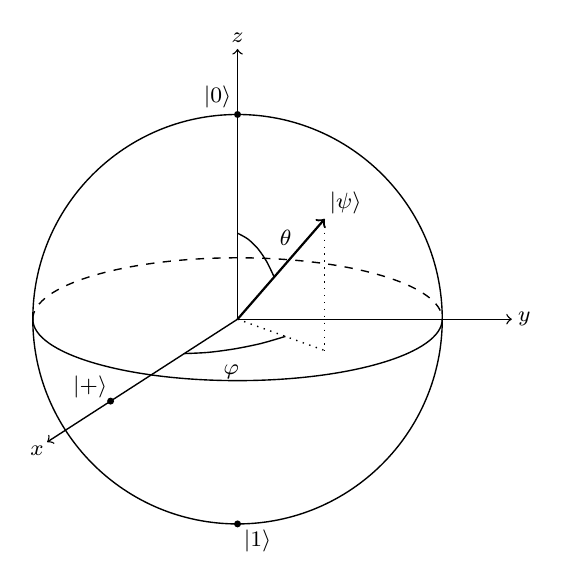
\begin{tikzpicture}[scale=2.6, line width=0.5pt]
	% sphere outline
	\draw (0,0) circle (1);
	% equator: back half dashed, front half solid
	\draw[dashed] (-1,0) arc[start angle=180, end angle=0, x radius=1, y radius=0.3];
	\draw (-1,0) arc[start angle=180, end angle=360, x radius=1, y radius=0.3];
	% axes
	\draw[->] (0,0) -- (0,1.32) node[above, inner sep=2pt] {\footnotesize $z$};
	\draw[->] (0,0) -- (1.34,0) node[right, inner sep=2pt] {\footnotesize $y$};
	\draw[->] (0,0) -- (-0.93,-0.60) node[below left, inner sep=1pt] {\footnotesize $x$};
	% state vector
	\draw[->, line width=0.8pt] (0,0) -- (0.426,0.490);
	\node[above right, inner sep=1.5pt] at (0.426,0.490) {\footnotesize $\ket{\psi}$};
	% projection to equatorial plane
	\draw[dotted] (0.426,0.490) -- (0.426,-0.153);
	\draw[dotted] (0,0) -- (0.426,-0.153);
	% angle theta (great circle from north pole to the state, radius 0.42)
	\draw plot[smooth] coordinates {(0,0.42) (0.050,0.392) (0.099,0.345) (0.142,0.282) (0.179,0.206)};
	\node at (0.235,0.40) {\footnotesize $\theta$};
	% angle phi (in the equatorial plane, radius 0.42)
	\draw plot[smooth] coordinates {(-0.260,-0.168) (-0.143,-0.162) (-0.015,-0.145) (0.113,-0.119) (0.234,-0.084)};
	\node at (-0.03,-0.255) {\footnotesize $\varphi$};
	% marked states
	\fill (0,1) circle (0.017);   \node[above left, inner sep=2pt] at (0,1) {\footnotesize $\ket{0}$};
	\fill (0,-1) circle (0.017);  \node[below right, inner sep=2pt] at (0,-1) {\footnotesize $\ket{1}$};
	\fill (-0.62,-0.40) circle (0.017); \node[above left, inner sep=1pt] at (-0.62,-0.40) {\footnotesize $\ket{+}$};
\end{tikzpicture}
\end{center}

The poles are $\ket{0}$ (north, $\theta = 0$) and $\ket{1}$ (south, $\theta = \pi$); the state $\ket{+}$ sits where the $x$-axis meets the equator, with $\ket{-}$ antipodal to it round the back; and $\tfrac{1}{\sqrt2}(\ket{0} \pm i \ket{1})$ sit at the two ends of the $y$-axis. The picture is a good source of intuition, but it comes with a warning attached: \emph{orthogonal states are antipodal, not perpendicular}. The angle between two states on the Bloch sphere is twice the angle between them in $\C^2$.

\begin{remark}
	The Bloch sphere is genuinely special to two dimensions. For a $d$-dimensional system the set of pure states is complex projective space $\CP^{d-1}$, which for $d = 2$ happens to be a $2$-sphere but for $d \geq 3$ has no such friendly picture. This is one reason why almost all of our concrete examples will be built from qubits.
\end{remark}

\subsection{Composite Systems and Tensor Products}

A single qubit is not much of a computer. To do anything interesting we need to combine systems, and the mathematical operation that does this is the tensor product.

\begin{definition}[Tensor Product]
	Let $\Vs$ and $\Ws$ be inner product spaces with orthonormal bases $\{\ket{e_1},\dots,\ket{e_m}\}$ and $\{\ket{f_1},\dots,\ket{f_n}\}$. Their \vocab{tensor product} $\Vs \otimes \Ws$ is the $mn$-dimensional space with orthonormal basis $\{\ket{e_i}\otimes\ket{f_j}\}_{i,j}$, and the map $(\ket{v},\ket{w}) \mapsto \ket{v}\otimes\ket{w}$ is extended bilinearly.
\end{definition}

Concretely, if $\ket{v}$ has components $(a_1,\dots,a_m)$ and $\ket{w}$ has components $(b_1,\dots,b_n)$, then $\ket{v}\otimes\ket{w}$ has the $mn$ components $a_i b_j$, listed in lexicographic order:
$$\ket{v} \otimes \ket{w} = (a_1b_1,\ a_1b_2,\ \dots,\ a_1 b_n,\ a_2b_1,\ \dots,\ a_mb_n)^{\mathsf T}.$$
The inner product on $\Vs \otimes \Ws$ is determined by
$$\left(\bra{v_1}\otimes\bra{w_1}\right)\left(\ket{v_2}\otimes\ket{w_2}\right) = \ip{v_1}{v_2}\ip{w_1}{w_2},$$
extended sesquilinearly; in components, if $\ket{A} = \sum_{ij} a_{ij}\ket{e_i}\ket{f_j}$ and $\ket{B} = \sum_{ij}b_{ij}\ket{e_i}\ket{f_j}$ then $\ip{A}{B} = \sum_{ij}a_{ij}^*b_{ij}$, as one would hope.

We will almost always drop the $\otimes$, writing $\ket{v}\ket{w}$, or even $\ket{vw}$, for $\ket{v}\otimes\ket{w}$. This is safe provided we remember that \emph{the order matters}: $\ket{v}\ket{w}$ and $\ket{w}\ket{v}$ live in $\Vs\otimes\Ws$ and $\Ws\otimes\Vs$ respectively, and even when $\Vs = \Ws$ they are different vectors. We also write $\Vs^{\otimes n}$ for the $n$-fold tensor power. If $\Vs = \C^2$ then $\Vs^{\otimes n}$ has dimension $2^n$, with orthonormal basis
$$\ket{i_1 i_2 \cdots i_n}, \qquad i_j \in \{0,1\},$$
indexed by the $2^n$ bit strings of length $n$. Note the exponential: $n$ qubits carry $2^n$ complex amplitudes.

We can now state the first two postulates of quantum mechanics in the form we will use them.

\begin{axiom}[States]
	To an isolated quantum system $S$ we associate a finite-dimensional inner product space $\Vs$. The states of $S$ are the rays of $\Vs$, represented by normalised vectors $\ket{\psi}$ determined up to a global phase.
\end{axiom}

\begin{axiom}[Composite Systems]
	If $S_1$ and $S_2$ are quantum systems with state spaces $\Vs_1$ and $\Vs_2$, then the composite system $S_1S_2$ has state space $\Vs_1 \otimes \Vs_2$.
\end{axiom}

The second postulate is where quantum mechanics diverges most sharply from classical intuition. Classically, the state of a pair of systems is a pair of states; the state space of the composite is the \emph{Cartesian product}, of dimension $m + n$. Quantum mechanically it is the tensor product, of dimension $mn$, and most of the vectors in it are not of the form $\ket{v}\ket{w}$ at all.

\begin{definition}[Product and Entangled States]
	A state $\ket{\Psi} \in \Vs \otimes \Ws$ is a \vocab{product state} if $\ket{\Psi} = \ket{\psi}\otimes\ket{\varphi}$ for some $\ket{\psi} \in \Vs$, $\ket{\varphi} \in \Ws$. Otherwise it is \vocab{entangled}.
\end{definition}

\begin{example}
	Let $\Vs = \Ws = \C^2$ and consider
	$$\ket{\phi^+} = \frac{1}{\sqrt2}\left(\ket{00} + \ket{11}\right).$$
	Suppose it were a product state, say $\ket{\phi^+} = (a\ket{0}+b\ket{1})\otimes(c\ket{0}+d\ket{1})$. Expanding,
	$$\ket{\phi^+} = ac\ket{00} + ad\ket{01} + bc\ket{10} + bd\ket{11},$$
	so we would need $ad = bc = 0$ and $ac = bd = 1/\sqrt2$. The latter forces all four of $a,b,c,d$ to be nonzero, contradicting the former. Hence $\ket{\phi^+}$ is entangled.
\end{example}

Counting parameters shows that entanglement is the norm rather than the exception: the product states of two qubits form a set of real dimension $2 + 2 = 4$ inside the $6$-real-dimensional set of all two-qubit states. Almost every state of a composite system is entangled, and the whole of \S\ref{sec:entanglement} is devoted to what one can do with that fact.

\subsection{Operators}

The Dirac notation extends painlessly to linear maps. If $A$ is a linear operator on $\Vs$ we write $A\ket{\psi}$ for its action, and $\bra{\psi}A\ket{\varphi}$ -- also written $\mel{\psi}{A}{\varphi}$ -- for the inner product of $\ket{\psi}$ with $A\ket{\varphi}$. There is a unique operator $A^\dagger$, the \vocab{adjoint}, satisfying
$$\ip{v}{Aw} = \ip{A^\dagger v}{w} \qquad \text{for all } \ket{v},\ket{w},$$
whose matrix is the conjugate transpose of that of $A$; one has $(AB)^\dagger = B^\dagger A^\dagger$, and with the convention $\ket{\psi}^\dagger = \bra{\psi}$ the rule `dagger reverses everything' holds universally. An operator with $A = A^\dagger$ is \vocab{self-adjoint} or \vocab{Hermitian}.

In a fixed basis, the outer products $\op{e_i}{e_j}$ are the matrix units, so any operator can be expanded as
$$A = \sum_{i,j} A_{ij} \op{e_i}{e_j}, \qquad A_{ij} = \mel{e_i}{A}{e_j}.$$
For a qubit this reads
$$A = \begin{pmatrix} a & b \\ c & d\end{pmatrix} = a \op{0}{0} + b\op{0}{1} + c\op{1}{0} + d\op{1}{1}.$$
Another identity worth recording is $\Tr\!\left(\op{v}{w}\right) = \ip{w}{v}$, and more generally $\Tr\!\left(A \op{\psi}{\psi}\right) = \mel{\psi}{A}{\psi}$; we will use this repeatedly to convert expectation values into traces, where they are easier to manipulate.

Four operators on $\C^2$ will appear on nearly every page.

\begin{definition}[Pauli Matrices]
	The \vocab{Pauli matrices} are
	$$\sigma_0 = I = \begin{pmatrix} 1 & 0 \\ 0 & 1 \end{pmatrix},\quad \sigma_x = \begin{pmatrix} 0 & 1 \\ 1 & 0\end{pmatrix},\quad \sigma_y = \begin{pmatrix} 0 & -i \\ i & 0\end{pmatrix},\quad \sigma_z = \begin{pmatrix} 1 & 0 \\ 0 & -1\end{pmatrix}.$$
\end{definition}

They are Hermitian, unitary and traceless, they square to the identity, and together with $I$ they form a basis of the space of $2\times 2$ complex matrices. Their action on the computational basis is
\begin{align*}
	\sigma_x \ket{0} &= \ket{1}, & \sigma_y\ket{0} &= i\ket{1}, & \sigma_z\ket{0} &= \ket{0},\\
	\sigma_x\ket{1} &= \ket{0}, & \sigma_y\ket{1} &= -i\ket{0}, & \sigma_z\ket{1} &= -\ket{1},
\end{align*}
so $\sigma_x$ is a bit flip, $\sigma_z$ is a phase flip, and $\sigma_y = i\sigma_x\sigma_z$ is both at once. They satisfy the cyclic relations
$$\sigma_x\sigma_y = i\sigma_z, \qquad \sigma_y\sigma_z = i\sigma_x, \qquad \sigma_z\sigma_x = i\sigma_y,$$
and any two distinct Pauli matrices anticommute. Geometrically, $\sigma_x, \sigma_y, \sigma_z$ generate rotations about the three axes of the Bloch sphere.

\subsection{Projectors}

Projection operators will carry all the weight in our discussion of measurement, so we set up the vocabulary now.

\begin{definition}[Projector]
	An operator $\Pi$ on $\Vs$ is a \vocab{(orthogonal) projector} if $\Pi^2 = \Pi$ and $\Pi^\dagger = \Pi$.
\end{definition}

If $\ket{v}$ is normalised then $\Pi_v = \op{v}{v}$ is a projector, since
$$\Pi_v\Pi_v = \op{v}{v}\op{v}{v} = \ket{v}\ip{v}{v}\bra{v} = \op{v}{v} = \Pi_v,$$
and $\Pi_v \ket{x} = \ket{v}\ip{v}{x}$ is the component of $\ket{x}$ along $\ket{v}$; in particular $\Pi_v$ kills everything orthogonal to $\ket{v}$. More generally, if $\Es \subseteq \Vs$ is a subspace with orthonormal basis $\ket{e_1},\dots,\ket{e_d}$, then
$$\Pi_{\Es} = \sum_{k=1}^d \op{e_k}{e_k}$$
is the orthogonal projector onto $\Es$, as one checks by extending to an orthonormal basis of $\Vs$. Its rank is $\dim \Es$, and $\Tr \Pi_{\Es} = \dim\Es$.

If $\Vs = \Es_1 \oplus \cdots \oplus \Es_d$ is an orthogonal direct sum decomposition, the corresponding projectors satisfy
$$\Pi_i \Pi_j = \delta_{ij}\Pi_i, \qquad \sum_{i=1}^d \Pi_i = I.$$
Such a family is exactly the data of a projective measurement, as we will see.

\subsection{Tensor Products of Operators}

Given linear maps $A$ on $\Vs$ and $B$ on $\Ws$, we define $A \otimes B$ on $\Vs\otimes\Ws$ by its action on product vectors,
$$(A\otimes B)\left(\ket{v}\otimes\ket{w}\right) = (A\ket{v})\otimes(B\ket{w}),$$
extended linearly. In components this is the familiar Kronecker product: for $2\times2$ matrices,
$$A = \begin{pmatrix} a & b \\ c & d\end{pmatrix},\ B = \begin{pmatrix} p & q \\ r & s\end{pmatrix} \implies A \otimes B = \begin{pmatrix} aB & bB \\ cB & dB\end{pmatrix} = \begin{pmatrix} ap & aq & bp & bq \\ ar & as & br & bs \\ cp & cq & dp & dq \\ cr & cs & dr & ds \end{pmatrix}.$$
The operators of the form $A \otimes I$ are those acting on the first system only, and $I \otimes B$ those acting on the second; these are the \vocab{local} operations, and the constraint that Alice and Bob can only perform local operations on their halves of a shared state is the central restriction in everything we do with entanglement.

\begin{example}
	Local operations act very differently on an entangled state than one might guess. With $\ket{\phi^+} = \tfrac{1}{\sqrt2}(\ket{00}+\ket{11})$ and $A$ as above,
	\begin{align*}
		(A\otimes I)\ket{\phi^+} &= \tfrac{1}{\sqrt2}\left[(A\ket{0})\ket{0} + (A\ket{1})\ket{1}\right] = \tfrac{1}{\sqrt2}\left[a\ket{00} + b\ket{01} + c\ket{10} + d\ket{11}\right], \\
		(I\otimes A)\ket{\phi^+} &= \tfrac{1}{\sqrt2}\left[\ket{0}(A\ket{0}) + \ket{1}(A\ket{1})\right] = \tfrac{1}{\sqrt2}\left[a\ket{00} + c\ket{01} + b\ket{10} + d\ket{11}\right].
	\end{align*}
	The two differ only by transposing $A$. In particular, for a symmetric $A$ we have $(A\otimes I)\ket{\phi^+} = (I\otimes A)\ket{\phi^+}$: acting on one half of a maximally entangled pair is the same as acting on the other. This innocuous-looking fact is the engine of superdense coding.
\end{example}

Finally, we record a construction that lets us `look at one half' of a composite state.

\begin{definition}[Partial Inner Product]
	Let $\ket{v} \in \Vs$. The \vocab{partial inner product} with $\ket{v}$ is the linear map $\Vs\otimes\Ws \to \Ws$ determined on the basis by
	$$\ket{e_i}\ket{f_j} \longmapsto \ip{v}{e_i}\ket{f_j}.$$
	We write it $\bra{v}$ again, so that $\bra{v}\left(\ket{\alpha}\ket{\beta}\right) = \ip{v}{\alpha}\ket{\beta}$.
\end{definition}

When $\Vs$ and $\Ws$ are isomorphic one must of course say which factor is meant, and we will do so by labelling the systems, writing $\bra{v}_A$ and so on. The notation is heavily overloaded but never actually ambiguous in practice.

\section{Measurement}

We now come to the part of the formalism with no classical analogue at all: what happens when we look at a quantum system. We state the remaining two postulates, extract the Born rule, and then answer the question that motivates the whole of quantum information theory -- \emph{when can two states be told apart?}

\subsection{Unitary Evolution}

\begin{axiom}[Evolution]
	The evolution of a closed quantum system over a finite time interval is given by a unitary operator on its state space: if the system is in state $\ket{\psi(t_1)}$ at time $t_1$, then at $t_2$ it is in state $\ket{\psi(t_2)} = U(t_1,t_2)\ket{\psi(t_1)}$ for some unitary $U(t_1,t_2)$ depending only on $t_1$ and $t_2$.
\end{axiom}

Recall from IA Vectors and Matrices that for a linear operator $U$ on a finite-dimensional inner product space the following are equivalent: $U^\dagger U = UU^\dagger = I$; $U$ preserves inner products, $\ip{Uv}{Uw} = \ip{v}{w}$; $U$ maps some (equivalently, every) orthonormal basis to an orthonormal basis; the columns of the matrix of $U$ form an orthonormal set.

The postulate is a consequence of the Schr\"odinger equation of IB Quantum Mechanics,
$$i\hbar \frac{\partial}{\partial t}\ket{\psi(t)} = H \ket{\psi(t)},$$
with $H$ the Hermitian Hamiltonian; for time-independent $H$ we get
$$U(t_1,t_2) = \exp\!\left(-\tfrac{i}{\hbar}H(t_2-t_1)\right),$$
which is unitary precisely because $H$ is Hermitian. In this course we will forget about Hamiltonians entirely and simply take `the allowed operations are the unitaries' as a black-box rule.

Two consequences deserve emphasis. First, unitary evolution is \emph{deterministic} and \emph{reversible}: the state at any time determines the state at any other. All the probability in quantum mechanics enters through measurement. Second, since unitaries preserve inner products, \emph{the overlap $\ip{\psi}{\varphi}$ between two states can never be changed by evolution}. Two states that start out non-orthogonal stay non-orthogonal forever, no matter what we do to them. Almost every impossibility theorem in this course is an application of that one sentence.

\subsection{Observables and the Born Rule}

\begin{definition}[Observable]
	An \vocab{observable} of a quantum system with state space $\Vs$ is a self-adjoint operator $A$ on $\Vs$.
\end{definition}

By the spectral theorem, a self-adjoint $A$ has real eigenvalues $a_1, \dots, a_k$ (which we take to be distinct) and $\Vs$ decomposes as an orthogonal direct sum of the corresponding eigenspaces. Writing $P_j$ for the projector onto the $a_j$-eigenspace, we obtain the \vocab{spectral decomposition}
$$A = \sum_j a_j P_j, \qquad P_iP_j = \delta_{ij}P_i, \qquad \sum_j P_j = I.$$
If $a_j$ is a non-degenerate eigenvalue with unit eigenvector $\ket{\varphi_j}$ then $P_j = \op{\varphi_j}{\varphi_j}$ has rank one; if $a_j$ has multiplicity $m$ then $P_j = \sum_{i=1}^m \op{\varphi_j^i}{\varphi_j^i}$ for an orthonormal basis of the eigenspace.

\begin{axiom}[Measurement; the Born Rule]
	If the observable $A = \sum_j a_j P_j$ is measured on a system in normalised state $\ket{\psi}$, the outcome is one of the eigenvalues $a_j$, obtained with probability
	$$p(a_j) = \mel{\psi}{P_j}{\psi} = \norm{P_j \ket{\psi}}^2,$$
	and the post-measurement state of the system is
	$$\frac{P_j\ket{\psi}}{\sqrt{p(a_j)}}.$$
\end{axiom}

Since $\sum_j P_j = I$ and $\ip{\psi}{\psi} = 1$, the probabilities do sum to one. A measurement of this form is called a \vocab{projective} or \vocab{von Neumann} measurement. Note that the state after the measurement is (the normalisation of) the projection of $\ket{\psi}$ onto the eigenspace we found -- the notorious `collapse of the wavefunction'. Measuring twice in a row gives the same answer both times, since $P_j$ applied to a vector already in its range does nothing.

In practice the eigenvalues themselves rarely matter; what matters is \emph{which} projector fired. So we will usually specify a measurement simply by giving the family of projectors, and speak of `the measurement $\{P_j\}$' with outcomes labelled by $j$.

\begin{definition}[Complete and Incomplete Measurements]
	A projective measurement $\{P_j\}$ is \vocab{complete} if every $P_j$ has rank $1$, and \vocab{incomplete} otherwise.
\end{definition}

A complete measurement is the same thing as a choice of orthonormal basis $\{\ket{e_j}\}$, with $P_j = \op{e_j}{e_j}$. Then, writing $\ket{\psi} = \sum_j a_j\ket{e_j}$,
$$p(j) = \abs{\ip{e_j}{\psi}}^2 = \abs{a_j}^2,$$
and the post-measurement state is
$$\frac{P_j\ket{\psi}}{\sqrt{p(j)}} = \frac{\ket{e_j}\ip{e_j}{\psi}}{\sqrt{p(j)}} = \ket{e_j}$$
up to a global phase. So the amplitudes really are amplitudes for outcomes, exactly as promised in \S1.1, and the state collapses onto a basis vector. We say we have \vocab{measured in the basis $\{\ket{e_j}\}$}.

An incomplete measurement corresponds instead to an orthogonal decomposition $\Vs = \Es_1 \oplus \cdots \oplus \Es_d$ into subspaces of arbitrary dimension: the outcome tells us which subspace, and the state collapses into that subspace but is not otherwise disturbed. It is a coarse-graining of a complete measurement, in the sense that if we refine each $\Es_i$ into an orthonormal basis and perform the complete measurement instead, then summing the probabilities of the outcomes lying in $\Es_i$ recovers $p(i)$.

\begin{example}[Parity Measurement]
	Take two qubits and decompose $\C^2\otimes\C^2 = \Es_0 \oplus \Es_1$, where
	$$\Es_0 = \vecspan\{\ket{00},\ket{11}\}, \qquad \Es_1 = \vecspan\{\ket{01},\ket{10}\}$$
	are the even- and odd-parity subspaces, `parity' meaning $b_1 \oplus b_2$. The corresponding measurement $\{\Pi_0, \Pi_1\}$ with $\Pi_0 = \op{00}{00}+\op{11}{11}$, $\Pi_1 = \op{01}{01}+\op{10}{10}$ tells us the parity of the two bits and nothing else. Applied to the state $\ket{\phi^+} = \tfrac{1}{\sqrt2}(\ket{00}+\ket{11})$ it returns $0$ with certainty and leaves the state untouched -- even though a complete measurement in the computational basis would destroy the entanglement completely. Measuring less can be worth more.
\end{example}

We will constantly want to measure a \emph{subsystem} of a composite system, and there is a useful special case of the Born rule for this.

\begin{proposition}[Extended Born Rule]
	Let $S_1S_2$ be a composite system with state spaces $\Vs$, $\Ws$ having complete orthonormal bases $\{\ket{e_i}\}_{i=1}^m$, $\{\ket{f_j}\}_{j=1}^n$, and let
	$$\ket{\psi} = \sum_{i,j} a_{ij}\ket{e_i}\ket{f_j}.$$
	Suppose we measure $S_1$ in the basis $\{\ket{e_i}\}$, that is, we perform the projective measurement with projectors $P_k \otimes I$, $P_k = \op{e_k}{e_k}$. Then the outcome is $k$ with probability
	$$p(k) = \mel{\psi}{P_k\otimes I}{\psi} = \sum_{j=1}^n \abs{a_{kj}}^2,$$
	and the post-measurement state is
	$$\ket{\psi_{\text{after}}} = \frac{(P_k\otimes I)\ket{\psi}}{\sqrt{p(k)}} = \ket{e_k}\otimes\frac{\sum_j a_{kj}\ket{f_j}}{\sqrt{\sum_j \abs{a_{kj}}^2}}.$$
\end{proposition}

\begin{proof}
	The projectors $P_k \otimes I$ project onto the mutually orthogonal subspaces $\Es_k = \ket{e_k}\otimes\Ws$, whose direct sum is $\Vs\otimes\Ws$, so this is a legitimate (in general incomplete) projective measurement. Expanding,
	$$\mel{\psi}{P_k \otimes I}{\psi} = \sum_{i,j}\sum_{i',j'}a_{ij}^*a_{i'j'}\ip{e_i}{e_k}\ip{e_k}{e_{i'}}\ip{f_j}{f_{j'}} = \sum_j \abs{a_{kj}}^2,$$
	using orthonormality. Applying $P_k\otimes I$ to $\ket{\psi}$ retains only the terms with $i = k$, giving $\ket{e_k}\otimes\sum_j a_{kj}\ket{f_j}$, and dividing by $\sqrt{p(k)}$ normalises it.
\end{proof}

Notice what the second half of this says: the state of $S_2$ after we measure $S_1$ depends on the outcome $k$. Measuring here changes the description of the state over there, instantaneously and no matter how far away it is. Whether this permits \emph{signalling} is a question we will settle -- in the negative -- in \S\ref{sec:nosignal}.

\begin{example}[Measuring One Qubit of Three]
	Let
	$$\ket{\psi} = \frac{i}{2}\ket{000} + \frac{1+i}{2\sqrt2}\ket{001} - \frac{1}{2}\ket{101} + \frac{3}{10}\ket{110} - \frac{2i}{5}\ket{111},$$
	which one checks is normalised: $\tfrac14 + \tfrac14 + \tfrac14 + \tfrac9{100} + \tfrac4{25} = 1$. Measure the first qubit in the computational basis. By the extended Born rule we sum $\abs{a}^2$ over the basis states beginning with $1$:
	$$p(1) = \frac14 + \frac{9}{100} + \frac{4}{25} = \frac{1}{2},$$
	so the outcome is $1$ with probability $\tfrac12$, and in that case the state becomes
	$$\ket{1}\otimes\frac{-\tfrac12\ket{01} + \tfrac3{10}\ket{10} - \tfrac{2i}5\ket{11}}{\sqrt{1/2}} = \ket{1}\otimes\left(-\tfrac{1}{\sqrt2}\ket{01} + \tfrac{3}{5\sqrt2}\ket{10} - \tfrac{4i}{5\sqrt2}\ket{11}\right).$$
\end{example}

\begin{remark}
	Measuring in an arbitrary basis is no more powerful than measuring in the computational basis, provided we may first apply a unitary. If $\Bs = \{\ket{e_i}\}$ and $\mathcal C = \{\ket{e_i'}\}$ are two orthonormal bases, let $U$ be the unitary with $U\ket{e_i} = \ket{e_i'}$. Measuring $\ket{\psi}$ in $\mathcal{C}$ gives outcome $i$ with probability
	$$\abs{\ip{e_i'}{\psi}}^2 = \abs{\bra{e_i}U^\dagger\ket{\psi}}^2,$$
	which is exactly the probability of outcome $i$ when $U^\dagger\ket{\psi}$ is measured in $\Bs$. So `apply $U^\dagger$, then measure in the standard basis' simulates any complete measurement, and we may as well assume that all measurements in a circuit are standard measurements.
\end{remark}

\subsection{Distinguishing Quantum States}\label{sec:distinguish}

Here is the question that separates quantum information from classical information theory. Someone hands us a system, promising that its state is either $\ket{\alpha_0}$ or $\ket{\alpha_1}$, both known to us. Can we determine which?

Classically the answer is trivially yes: distinct classical states are distinct, and looking tells you which. Quantum mechanically the answer is a sharp and surprising one.

\begin{definition}[Reliably Distinguishable]
	Two states $\ket{\psi},\ket{\varphi}$ are \vocab{reliably distinguishable} if there is a measurement with two distinguished outcomes $0,1$ such that measuring $\ket{\psi}$ gives outcome $0$ with probability $1$, and measuring $\ket{\varphi}$ gives outcome $1$ with probability $1$.
\end{definition}

\begin{theorem}
	Two states $\ket{\psi}$ and $\ket{\varphi}$ are reliably distinguishable if and only if $\ip{\psi}{\varphi} = 0$.
\end{theorem}

\begin{proof}
	Suppose first that $\ip{\psi}{\varphi} = 0$. Extend $\ket{\psi}$ to a complete orthonormal basis $\{\ket{\psi}, \ket{f_1},\dots,\ket{f_{m-1}}\}$ of $\Vs$ and consider the incomplete measurement $\{\Pi_0, \Pi_1\}$ with $\Pi_0 = \op{\psi}{\psi}$ and $\Pi_1 = I - \Pi_0$. Then measuring $\ket{\psi}$ gives outcome $0$ with probability $\mel{\psi}{\Pi_0}{\psi} = 1$, while measuring $\ket{\varphi}$ gives outcome $0$ with probability $\abs{\ip{\psi}{\varphi}}^2 = 0$, hence outcome $1$ with certainty.

	Conversely, suppose such a measurement $\{\Pi_0, \Pi_1, \dots\}$ exists. Then $\mel{\psi}{\Pi_0}{\psi} = 1$ forces $\Pi_0\ket{\psi} = \ket{\psi}$, since $\norm{\Pi_0\ket{\psi}}^2 = 1 = \norm{\ket{\psi}}^2$ and $\Pi_0$ is a contraction which fixes a unit vector only if that vector lies in its range. Similarly $\mel{\varphi}{\Pi_1}{\varphi} = 1$ gives $\Pi_1\ket{\varphi} = \ket{\varphi}$. But the ranges of $\Pi_0$ and $\Pi_1$ are orthogonal subspaces, so
	$$\ip{\psi}{\varphi} = \ip{\Pi_0\psi}{\Pi_1\varphi} = \mel{\psi}{\Pi_0\Pi_1}{\varphi} = 0. \qedhere$$
\end{proof}

So non-orthogonal states cannot be told apart with certainty, ever, by any measurement. Note also the trivial but important corollary that $\ket{\psi}$ and $e^{i\theta}\ket{\psi}$ are indistinguishable, which is what justified our identification of states with rays.

What if we allow ourselves to be wrong sometimes? Suppose the two candidate states are equally likely a priori and we must guess. We could ignore the system entirely and flip a coin, succeeding with probability $\tfrac12$. Can we do better, and how much better?

Before answering, note that there is no point being clever about the \emph{form} of the measurement. If we adjoin an ancilla in a fixed state $\ket{A}$, apply a unitary $U$ to the enlarged system and then measure with $\{\Pi_i\}$, the outcome probabilities are
$$p(i) = \mel{\alpha_j A}{U^\dagger \Pi_i U}{\alpha_j A},$$
and $\{U^\dagger \Pi_i U\}$ is again a family of orthogonal projectors summing to the identity. So the whole procedure is just \emph{some} projective measurement performed directly on $\ket{\alpha_j}\ket{A}$; and since the ancilla contributes the same factor $\ip{A}{A} = 1$ in both cases, we may as well restrict attention to two-outcome projective measurements $\{\Pi_0,\Pi_1\}$ on the original system, with $\Pi_0 + \Pi_1 = I$. We guess $\ket{\alpha_0}$ on outcome $0$ and $\ket{\alpha_1}$ on outcome $1$.

\begin{theorem}[Holevo--Helstrom, Pure States]
	Let $\ket{\alpha_0},\ket{\alpha_1}$ be given with equal prior probabilities $\tfrac12$, and write $\abs{\ip{\alpha_0}{\alpha_1}} = \cos\theta$ with $\theta \in [0,\pi/2]$. Then the average success probability of any measurement strategy satisfies
	$$p_S \leq \frac{1}{2} + \frac{\sin\theta}{2},$$
	and there is a measurement attaining this bound.
\end{theorem}

\begin{proof}
	With the two-outcome measurement $\{\Pi_0,\Pi_1 = I - \Pi_0\}$ the average success probability is
	\begin{align*}
		p_S &= \tfrac12\mel{\alpha_0}{\Pi_0}{\alpha_0} + \tfrac12\mel{\alpha_1}{\Pi_1}{\alpha_1}\\
		&= \tfrac12\mel{\alpha_0}{\Pi_0}{\alpha_0} + \tfrac12\left(1 - \mel{\alpha_1}{\Pi_0}{\alpha_1}\right) \\
		&= \frac12 + \frac12\Tr\!\left[\Pi_0 \Delta\right], \qquad \Delta := \op{\alpha_0}{\alpha_0} - \op{\alpha_1}{\alpha_1},
	\end{align*}
	where we used $\mel{\psi}{A}{\psi} = \Tr(A\op{\psi}{\psi})$. So we must maximise $\Tr(\Pi_0\Delta)$ over projectors $\Pi_0$.

	Now $\Delta$ is self-adjoint, so it has real eigenvalues and an orthonormal eigenbasis. It annihilates every vector orthogonal to both $\ket{\alpha_0}$ and $\ket{\alpha_1}$, so it acts nontrivially only on $\vecspan\{\ket{\alpha_0},\ket{\alpha_1}\}$, and has at most two nonzero eigenvalues. Also $\Tr\Delta = 1 - 1 = 0$, so those eigenvalues are $\delta$ and $-\delta$ for some $\delta \geq 0$; write $\ket{p}, \ket{m}$ for corresponding orthonormal eigenvectors, so
	$$\Delta = \delta\op{p}{p} - \delta\op{m}{m}.$$

	To find $\delta$, pick a normalised $\ket{\alpha_0^\perp} \in \vecspan\{\ket{\alpha_0},\ket{\alpha_1}\}$ orthogonal to $\ket{\alpha_0}$, so that $\{\ket{\alpha_0}, \ket{\alpha_0^\perp}\}$ is an orthonormal basis of that plane, and write $\ket{\alpha_1} = c_0\ket{\alpha_0} + c_1\ket{\alpha_0^\perp}$ with $\abs{c_0}^2 + \abs{c_1}^2 = 1$. In this basis
	$$\Delta = \begin{pmatrix} 1 & 0 \\ 0 & 0\end{pmatrix} - \begin{pmatrix} \abs{c_0}^2 & c_0c_1^* \\ c_0^*c_1 & \abs{c_1}^2 \end{pmatrix} = \begin{pmatrix} \abs{c_1}^2 & -c_0c_1^* \\ -c_0^*c_1 & -\abs{c_1}^2\end{pmatrix},$$
	whose determinant is $-\abs{c_1}^4 - \abs{c_0}^2\abs{c_1}^2 = -\abs{c_1}^2$. Since the eigenvalues are $\pm\delta$, their product is $-\delta^2$, so $\delta = \abs{c_1}$. But $\abs{c_0} = \abs{\ip{\alpha_0}{\alpha_1}} = \cos\theta$, so $\delta = \sin\theta$.

	Therefore
	$$p_S = \frac12 + \frac{\sin\theta}{2}\left[\mel{p}{\Pi_0}{p} - \mel{m}{\Pi_0}{m}\right].$$
	For any projector and any unit vector, $0 \leq \mel{\varphi}{\Pi_0}{\varphi} \leq 1$, so the bracket is at most $1$, giving $p_S \leq \tfrac12 + \tfrac{\sin\theta}{2}$. Equality holds when $\mel{p}{\Pi_0}{p} = 1$ and $\mel{m}{\Pi_0}{m} = 0$, which is achieved by the choice $\Pi_0 = \op{p}{p}$, $\Pi_1 = I - \op{p}{p}$.
\end{proof}

The geometry is worth drawing. In the plane spanned by the two states, $\ket{\alpha_0}$ and $\ket{\alpha_1}$ subtend an angle $\tfrac{\pi}{2} - \theta$; the optimal measurement basis $\{\ket{p},\ket{m}\}$ is the pair of orthogonal directions that `straddles' them symmetrically.

\begin{center}
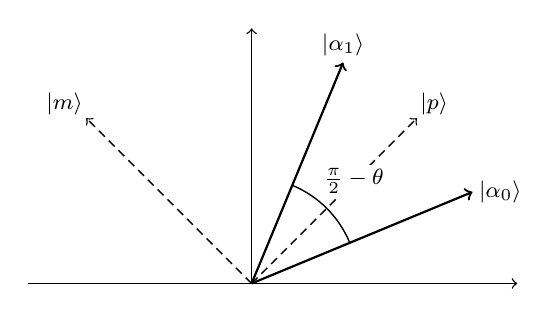
\begin{tikzpicture}[scale=2.7, line width=0.5pt]
	\draw[->] (-1.05,0) -- (1.25,0);
	\draw[->] (0,0) -- (0,1.20);
	% alpha_0 at 22.5 deg, alpha_1 at 67.5 deg (angle between them = 45 = pi/2 - theta, so theta = pi/4)
	\draw[->, line width=0.8pt] (0,0) -- (1.0392,0.4306) node[right, inner sep=2pt] {\footnotesize $\ket{\alpha_0}$};
	\draw[->, line width=0.8pt] (0,0) -- (0.4306,1.0392) node[above, inner sep=2pt] {\footnotesize $\ket{\alpha_1}$};
	% p bisects them at 45 deg, m orthogonal to p at 135
	\draw[->, densely dashed] (0,0) -- (0.7778,0.7778) node[above right, inner sep=1pt] {\footnotesize $\ket{p}$};
	\draw[->, densely dashed] (0,0) -- (-0.7778,0.7778) node[above left, inner sep=1pt] {\footnotesize $\ket{m}$};
	% arc between the two states
	\draw (0.4619,0.1913) arc[start angle=22.5, end angle=67.5, radius=0.5];
	\node[fill=white, inner sep=1.5pt] at (0.481,0.481) {\footnotesize $\frac{\pi}{2}-\theta$};
\end{tikzpicture}
\end{center}

Two sanity checks. If the states are orthogonal, $\theta = \pi/2$ and the bound reads $p_S \le 1$, attained: this is the theorem above. If the states are equal, $\theta = 0$ and $p_S \leq \tfrac12$: we can do no better than guessing, as we must. And in between we interpolate smoothly. There is no sharp line between `distinguishable' and `indistinguishable'; there is a continuum, governed entirely by the overlap $\abs{\ip{\alpha_0}{\alpha_1}}$.

\section{No Cloning and No Signalling}

Having established what quantum states can do, we now establish two things that they cannot do. Both are one-line consequences of linearity, and both turn out to be indispensable: the first is what makes quantum cryptography possible, and the second is what stops quantum mechanics from contradicting relativity.

\subsection{Going to the Church of the Higher Hilbert Space}

Before proving impossibility results we should be careful about what we are allowed to try. The most general thing we can do to a system $S$ in state $\ket{\psi}$ is:
\begin{enumerate}[label=(\roman*)]
	\item \emph{(ancilla)} adjoin an auxiliary system $A$ in a fixed state $\ket{A}$, so that the joint state of $SA$ is $\ket{\psi}\ket{A} \in \Vs_S \otimes \Vs_A$;
	\item \emph{(unitary)} apply a unitary $U$ to the whole of $SA$;
	\item \emph{(measure)} perform a measurement on $SA$, keep the post-measurement state of $S$, and discard $A$.
\end{enumerate}
This is often called \emph{going to the church of the higher Hilbert space}: any messy, noisy, irreversible-looking process on $S$ can be modelled as a clean unitary evolution on a larger closed system, followed by throwing part of it away. The point of the ancilla is not merely bookkeeping -- it provides somewhere for $S$ to become entangled \emph{with}, which is exactly how information leaks out of a system in practice.

We will therefore prove our impossibility theorems in this general setting, and they will apply to any physical process whatsoever.

\subsection{The No-Cloning Theorem}

Classical information can be copied freely: read the bit, write it down again. Can quantum information be copied? A copier would be a device that takes the state $\ket{\psi}$ we want to duplicate, a blank system $B$ initially in some fixed state $\ket{0}$, and a machine $M$ in some fixed `ready' state $\ket{M_0}$, and produces two copies of $\ket{\psi}$:
$$\ket{\psi}_A\ket{0}_B\ket{M_0}_M \longmapsto \ket{\psi}_A\ket{\psi}_B\ket{M_\psi}_M.$$
Note that the machine is allowed to end up in a state $\ket{M_\psi}$ that depends on what was copied -- we are not demanding that it be reset.

\begin{center}
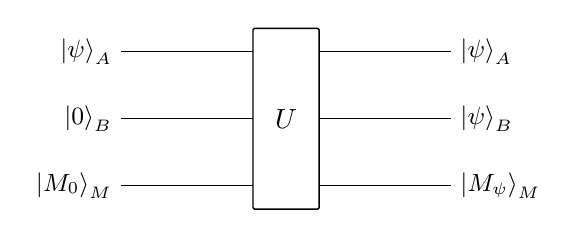
\begin{tikzpicture}[x=1.05cm, y=0.85cm, line width=0.5pt]
	\draw (0,0) -- (1.6,0);   \draw (0,-1) -- (1.6,-1);   \draw (0,-2) -- (1.6,-2);
	\draw (2.4,0) -- (4.0,0); \draw (2.4,-1) -- (4.0,-1); \draw (2.4,-2) -- (4.0,-2);
	\filldraw[fill=white, rounded corners=0.5pt] (1.6,0.35) rectangle (2.4,-2.35);
	\node at (2.0,-1) {$U$};
	\node[left, inner sep=3pt, font=\small] at (0,0) {$\ket{\psi}_A$};
	\node[left, inner sep=3pt, font=\small] at (0,-1) {$\ket{0}_B$};
	\node[left, inner sep=3pt, font=\small] at (0,-2) {$\ket{M_0}_M$};
	\node[right, inner sep=3pt, font=\small] at (4.0,0) {$\ket{\psi}_A$};
	\node[right, inner sep=3pt, font=\small] at (4.0,-1) {$\ket{\psi}_B$};
	\node[right, inner sep=3pt, font=\small] at (4.0,-2) {$\ket{M_\psi}_M$};
\end{tikzpicture}
\end{center}

\begin{theorem}[No-Cloning Theorem]
	Let $\Ss$ be any set of states of a system $A$ containing at least one pair of distinct non-orthogonal states. Then there is no unitary\footnote{And hence no process at all: by the discussion of \S3.1, a general process is a unitary on a larger system followed by a measurement, and we may let $M$ absorb both the ancilla and, by the principle of deferred measurement, any measurement performed.} $U$ which clones every state in $\Ss$.
\end{theorem}

\begin{proof}
	Let $\ket{\xi}, \ket{\eta} \in \Ss$ be distinct and non-orthogonal, so that $0 < \abs{\ip{\xi}{\eta}} < 1$. Suppose such a $U$ existed. Then
	$$U\ket{\xi}_A\ket{0}_B\ket{M_0}_M = \ket{\xi}_A\ket{\xi}_B\ket{M_\xi}_M, \qquad U\ket{\eta}_A\ket{0}_B\ket{M_0}_M = \ket{\eta}_A\ket{\eta}_B\ket{M_\eta}_M.$$
	Unitaries preserve inner products, so taking the inner product of the two left-hand sides and of the two right-hand sides must give the same answer. The inner product on a tensor product factorises, so
	$$\ip{\xi}{\eta}\ip{0}{0}\ip{M_0}{M_0} = \ip{\xi}{\eta}\ip{\xi}{\eta}\ip{M_\xi}{M_\eta},$$
	that is, $\ip{\xi}{\eta} = \ip{\xi}{\eta}^2 \ip{M_\xi}{M_\eta}$. Taking absolute values and dividing by $\abs{\ip{\xi}{\eta}} \neq 0$ gives
	$$1 = \abs{\ip{\xi}{\eta}}\,\abs{\ip{M_\xi}{M_\eta}}.$$
	But $\abs{\ip{\xi}{\eta}} < 1$ and $\abs{\ip{M_\xi}{M_\eta}} \leq 1$ by Cauchy--Schwarz, so the right-hand side is strictly less than $1$. This is a contradiction.
\end{proof}

The theorem is sharp in both directions. A set of \emph{mutually orthogonal} states \emph{can} be cloned: extend them to an orthonormal basis $\{\ket{e_i}\}$ and let $U$ be any unitary with $U\ket{e_i}\ket{0} = \ket{e_i}\ket{e_i}$, which exists because the images are orthonormal. This is exactly the statement that \emph{classical} information -- information encoded in orthogonal states -- can be copied. It is the superposition states in between that resist duplication.

\begin{remark}
	It is worth noticing which feature of quantum mechanics is doing the work. It is linearity, nothing else. If $U\ket{\psi}\ket{0} = \ket{\psi}\ket{\psi}$ for all $\ket{\psi}$, then the left-hand side is linear in $\ket{\psi}$ and the right-hand side is quadratic, and the two cannot agree.
\end{remark}

Why should we care? Suppose we could clone. Then we could take an unknown state, make a million copies, and measure them all in different bases, thereby learning the state to arbitrary precision from a single copy. But the amplitudes of an unknown state are continuous parameters, so a single qubit would carry an unbounded amount of extractable classical information. That would be strange enough. In fact, it is worse.

\subsection{Cloning Would Permit Superluminal Signalling}

Suppose Alice and Bob each hold one qubit of the entangled state
$$\ket{\phi^+}_{AB} = \frac{1}{\sqrt2}\left(\ket{00} + \ket{11}\right),$$
and are separated by a light-year. Alice wants to send Bob one bit \emph{now}. Here is her protocol. To send `yes', she measures her qubit in the basis $\{\ket{0},\ket{1}\}$; to send `no', she measures it in the basis $\{\ket{+},\ket{-}\}$.

Consider what happens to Bob's qubit. Writing $\ket{\phi^+}$ in the conjugate basis,
$$\ket{\phi^+} = \frac{1}{\sqrt2}\left(\ket{00}+\ket{11}\right) = \frac{1}{\sqrt2}\left(\ket{++} + \ket{--}\right),$$
as one checks by expanding. So by the extended Born rule, if Alice measures in the standard basis then with probability $\tfrac12$ each Bob's qubit is left in the state $\ket{0}$ or $\ket{1}$; if she measures in the conjugate basis then with probability $\tfrac12$ each it is left in $\ket{+}$ or $\ket{-}$.

Bob therefore holds a qubit prepared in one of two \emph{ensembles}: an equal mixture of $\{\ket{0},\ket{1}\}$, or an equal mixture of $\{\ket{+},\ket{-}\}$. If he could tell these ensembles apart, he would learn Alice's bit instantly. But he cannot: for any measurement $\{\Pi_i\}$ on his qubit,
$$p_{\text{yes}}(i) = \tfrac12\mel{0}{\Pi_i}{0} + \tfrac12\mel{1}{\Pi_i}{1} = \tfrac12\Tr\!\left[\Pi_i\left(\op{0}{0}+\op{1}{1}\right)\right] = \tfrac12 \Tr \Pi_i,$$
$$p_{\text{no}}(i) = \tfrac12\mel{+}{\Pi_i}{+} + \tfrac12\mel{-}{\Pi_i}{-} = \tfrac12\Tr\!\left[\Pi_i\left(\op{+}{+}+\op{-}{-}\right)\right] = \tfrac12\Tr\Pi_i,$$
since both $\op{0}{0}+\op{1}{1}$ and $\op{+}{+}+\op{-}{-}$ equal the identity. The two probability distributions are \emph{identical}, whatever measurement Bob makes. No signal.

But now suppose Bob could clone. He makes $N$ copies of his qubit and measures each in the standard basis. If Alice sent `yes', his qubit was $\ket{0}$ or $\ket{1}$, so all $N$ outcomes agree. If she sent `no', his qubit was $\ket{\pm}$, and each of the $N$ measurements gives $0$ or $1$ independently and uniformly, so the probability that they all agree is $2\cdot 2^{-N} = 2^{-N+1}$. Bob declares `yes' if the outcomes agree and `no' otherwise, and is wrong with probability at most $2^{-N+1}$, which he can make as small as he likes.

So cloning would give instantaneous communication across arbitrary distances, in flat contradiction with special relativity. The no-cloning theorem is not a technical curiosity; it is what keeps quantum mechanics consistent with the rest of physics.

\subsection{The No-Signalling Principle}\label{sec:nosignal}

The argument above shows that Bob cannot detect Alice's \emph{choice of basis}. In fact something much stronger is true: Bob cannot detect \emph{whether Alice measured at all}.

\begin{theorem}[No-Signalling Principle]
	Let $\ket{\phi_{AB}} \in \Vs_A \otimes \Vs_B$ be an arbitrary (possibly entangled) state shared by Alice and Bob, and let Bob perform a complete measurement in a basis $\{\ket{b}\}$ of $\Vs_B$. The probability distribution of Bob's outcome is the same whether or not Alice first performs a measurement on her system, and is independent of which measurement she performs.
\end{theorem}

\begin{proof}
	Fix a complete orthonormal basis $\{\ket{a}\}$ of $\Vs_A$, expand $\ket{\phi_{AB}} = \sum_{a,b} c_{ab}\ket{a}\ket{b}$, and write $P_a = \op{a}{a}$, $P_b = \op{b}{b}$.

	If Alice does nothing, the extended Born rule gives Bob outcome $b$ with probability
	$$p(b) = \mel{\phi_{AB}}{I_A\otimes P_b}{\phi_{AB}} = \sum_a \abs{c_{ab}}^2.$$

	Suppose instead Alice first measures in the basis $\{\ket{a}\}$. She gets outcome $a$ with probability $p(a) = \sum_b\abs{c_{ab}}^2$, and the joint state becomes
	$$\ket{\phi''_{AB}} = \frac{(P_a\otimes I_B)\ket{\phi_{AB}}}{\sqrt{p(a)}}.$$
	Bob's conditional probability of outcome $b$ is then
	\begin{align*}
		p(b \mid a) &= \mel{\phi''_{AB}}{I_A\otimes P_b}{\phi''_{AB}} \\
		&= \frac{1}{p(a)}\mel{\phi_{AB}}{(P_a\otimes I)(I\otimes P_b)(P_a\otimes I)}{\phi_{AB}} \\
		&= \frac{1}{p(a)}\mel{\phi_{AB}}{P_a\otimes P_b}{\phi_{AB}},
	\end{align*}
	using $P_a^2 = P_a$ and the fact that operators on different factors commute. Hence the joint distribution is $p(a,b) = p(a)p(b\mid a) = \mel{\phi_{AB}}{P_a\otimes P_b}{\phi_{AB}} = \abs{c_{ab}}^2$, and Bob's marginal is
	$$\sum_a p(a,b) = \sum_a \abs{c_{ab}}^2 = p(b),$$
	exactly as before. Since Alice measuring in any other basis is the same as applying a unitary to her half and then measuring in $\{\ket{a}\}$, and unitaries of the form $U \otimes I$ leave Bob's marginal alone by the same computation, the result is independent of her choice.
\end{proof}

So the `collapse' induced at a distance is real as a change in our \emph{description} of Bob's system, but it carries no information whatsoever. It is only when Alice tells Bob, over an ordinary classical channel, what she did and what she got, that the correlations become visible. Every protocol in this course respects this: teleportation, superdense coding and key distribution all require classical communication, and all are therefore limited by the speed of light.

\section{Entanglement}\label{sec:entanglement}

Entanglement is the resource that makes quantum information interesting. In this section we meet the canonical entangled states, and then confront the fact -- established by Bell, and by now verified experimentally beyond any reasonable doubt -- that the correlations they exhibit cannot be reproduced by \emph{any} classical mechanism.

\subsection{The Bell Basis}

\begin{definition}[Bell States]
	The \vocab{Bell states} of a pair of qubits are
	$$\ket{\phi^\pm} = \frac{1}{\sqrt2}\left(\ket{00}\pm\ket{11}\right), \qquad \ket{\psi^\pm} = \frac{1}{\sqrt2}\left(\ket{01}\pm\ket{10}\right).$$
	They form an orthonormal basis of $\C^2\otimes\C^2$, the \vocab{Bell basis}.
\end{definition}

Orthonormality is immediate from the orthonormality of the computational basis. Each Bell state is entangled, by the same argument we gave for $\ket{\phi^+}$. They are also \vocab{maximally} entangled, in a sense we can make precise here informally: measuring either qubit alone in \emph{any} basis gives a uniformly random outcome, so an observer with access to one qubit has no information at all, while the pair together is in a perfectly definite state. All of the information is in the correlations.

These states are also known as \vocab{EPR pairs}, after the 1935 paper of Einstein, Podolsky and Rosen, who considered a state of this kind and argued that quantum mechanics must be incomplete. Their reasoning, in modern dress: measuring Alice's qubit of $\ket{\phi^+}$ in the standard basis determines Bob's outcome with certainty, and by no-signalling this cannot be a physical influence; so Bob's outcome must have been predetermined by some \emph{element of reality} which the quantum state fails to record. Call such a hidden parameter $\lambda$. EPR concluded that the wavefunction is an incomplete description of reality. It was thirty years before Bell showed that this conclusion is not merely unnecessary but \emph{false}.

Before we get there, a computational fact which we will use constantly.

\begin{proposition}
	Write $X = \sigma_x$, $Z = \sigma_z$ and $Y = i\sigma_y = \begin{psmallmatrix} 0 & 1 \\ -1 & 0\end{psmallmatrix}$. Then all four Bell states are obtained from $\ket{\phi^+}$ by a local operation on the first qubit:
	\begin{align*}
		\ket{\phi^+} &= (I\otimes I)\ket{\phi^+}, & \ket{\phi^-} &= (Z\otimes I)\ket{\phi^+},\\
		\ket{\psi^+} &= (X\otimes I)\ket{\phi^+}, & \ket{\psi^-} &= (Y\otimes I)\ket{\phi^+}.
	\end{align*}
	The same holds with the operators acting on the second qubit instead, except that $\ket{\psi^-} = -(I\otimes Y)\ket{\phi^+}$.
\end{proposition}

\begin{proof}
	Direct computation. For instance
	$$(X\otimes I)\ket{\phi^+} = \tfrac{1}{\sqrt2}\left((X\ket{0})\ket{0} + (X\ket{1})\ket{1}\right) = \tfrac{1}{\sqrt2}\left(\ket{10}+\ket{01}\right) = \ket{\psi^+},$$
	and
	$$(Y\otimes I)\ket{\phi^+} = \tfrac1{\sqrt2}\left((Y\ket{0})\ket{0} + (Y\ket{1})\ket{1}\right) = \tfrac1{\sqrt2}\left(-\ket{10}+\ket{01}\right) = \ket{\psi^-},$$
	since $Y\ket{0} = -\ket{1}$ and $Y\ket{1} = \ket{0}$. The remaining cases are similar, and the statements for the second qubit follow from the example of \S1.7, since $I,X,Z$ are symmetric matrices and $Y$ is antisymmetric.
\end{proof}

The moral is striking: Alice, acting only on her own qubit, can steer the joint state to any of four mutually orthogonal -- and hence perfectly distinguishable -- states. She has two bits of leverage over a system she only half owns. We will cash this in as superdense coding in \S6.

\subsection{Bell Inequalities and the CHSH Game}

Let us take the EPR argument seriously and ask what a \emph{local hidden variable} theory would predict. The setup: Alice and Bob are far apart, sharing some system. Alice chooses one of two binary-outcome measurements, labelled by $s \in \{0,1\}$, and obtains an outcome $a \in \{-1,+1\}$; Bob chooses $t \in \{0,1\}$ and gets $b \in \{-1,+1\}$. The experiment is repeated many times and they compare notes, computing the four correlations $\EE[ab \mid s,t]$.

A \vocab{local hidden variable} (LHV) model asserts that there is a random variable $\lambda$, distributed according to some law $p(\lambda)$, and functions
$$A_0(\lambda), A_1(\lambda), B_0(\lambda), B_1(\lambda) \in \{-1,+1\}$$
such that Alice's outcome for setting $s$ is $A_s(\lambda)$ and Bob's for setting $t$ is $B_t(\lambda)$. \emph{Locality} is the assumption that $A_s$ does not depend on $t$ and vice versa -- Alice's outcome cannot depend on a choice made outside her light cone. \emph{Realism} is the assumption that all four values exist simultaneously, even though only two of them are measured in any given run.

\begin{theorem}[CHSH Inequality]
	In any local hidden variable model, the quantity
	$$S = \EE[A_0B_0] + \EE[A_0B_1] + \EE[A_1B_0] - \EE[A_1B_1]$$
	satisfies $\abs{S} \leq 2$.
\end{theorem}

\begin{proof}
	Fix $\lambda$ and consider
	\begin{align*}
		&A_0(\lambda)B_0(\lambda) + A_0(\lambda)B_1(\lambda) + A_1(\lambda)B_0(\lambda) - A_1(\lambda)B_1(\lambda) \\
		&\qquad = A_0(\lambda)\left[B_0(\lambda)+B_1(\lambda)\right] + A_1(\lambda)\left[B_0(\lambda)-B_1(\lambda)\right].
	\end{align*}
	Since $B_0(\lambda), B_1(\lambda) \in \{-1,+1\}$, one of $B_0+B_1$ and $B_0 - B_1$ is $0$ and the other is $\pm2$. Hence the whole expression is $\pm 2 A_s(\lambda)$ for one of $s = 0,1$, and so lies in $\{-2,+2\}$. Averaging over $\lambda$ with respect to $p(\lambda)$ and using linearity of expectation gives $\abs{S}\leq 2$.
\end{proof}

The inequality is a genuine constraint on the observable correlations, derived from nothing but locality and realism. And quantum mechanics violates it.

\begin{theorem}[Quantum Violation of CHSH]
	Let Alice and Bob share the state $\ket{\psi^-} = \tfrac{1}{\sqrt2}(\ket{01}-\ket{10})$, and let each measure the spin observable along a direction in a fixed plane: Alice measures $A(\alpha) = \cos\alpha\, \sigma_z + \sin\alpha\,\sigma_x$ and Bob measures $B(\beta) = \cos\beta\,\sigma_z + \sin\beta\,\sigma_x$. Then
	$$\EE\!\left[A(\alpha)B(\beta)\right] = -\cos(\alpha-\beta),$$
	and with the choices $\alpha_0 = 0$, $\alpha_1 = \tfrac{\pi}{2}$, $\beta_0 = \tfrac{\pi}{4}$, $\beta_1 = -\tfrac{\pi}{4}$ we obtain
	$$S = -2\sqrt2, \qquad \abs{S} = 2\sqrt{2} > 2.$$
\end{theorem}

\begin{proof}
	Each $A(\alpha)$ is Hermitian with $A(\alpha)^2 = I$ (using $\sigma_z^2 = \sigma_x^2 = I$ and $\sigma_z\sigma_x + \sigma_x\sigma_z = 0$), so its eigenvalues are $\pm1$ and it is a legitimate $\pm1$-valued observable. The correlation is the expectation of the observable $A(\alpha)\otimes B(\beta)$ in the state $\ket{\psi^-}$.

	We use the fact that $\ket{\psi^-}$ is \emph{rotationally invariant}: for any $2\times2$ unitary $U$ with $\det U = 1$ we have $(U \otimes U)\ket{\psi^-} = \ket{\psi^-}$, because $\ket{\psi^-}$ spans the antisymmetric part of $\C^2\otimes\C^2$ and $U \otimes U$ acts on it by $\det U$. Rather than invoke this, though, let us simply compute. Write $\ket{\psi^-} = \tfrac1{\sqrt2}(\ket{01}-\ket{10})$ and note the useful identities
	$$\sigma_z\otimes\sigma_z\ket{\psi^-} = -\ket{\psi^-}, \qquad \sigma_x\otimes\sigma_x\ket{\psi^-} = -\ket{\psi^-},$$
	the first because $\sigma_z\otimes\sigma_z\ket{01} = -\ket{01}$ and likewise for $\ket{10}$; the second because $\sigma_x\otimes\sigma_x$ swaps $\ket{01}\leftrightarrow\ket{10}$, which negates the antisymmetric combination. We also need the cross terms:
	$$\left(\sigma_z\otimes\sigma_x\right)\ket{\psi^-} = \tfrac1{\sqrt2}\left(\ket{00} + \ket{11}\right) = \ket{\phi^+},$$
	since $\sigma_z\otimes\sigma_x\ket{01} = \ket{00}$ and $\sigma_z\otimes\sigma_x\ket{10} = -\ket{11}$. As $\ip{\psi^-}{\phi^+} = 0$, we get $\mel{\psi^-}{\sigma_z\otimes\sigma_x}{\psi^-} = 0$, and symmetrically $\mel{\psi^-}{\sigma_x\otimes\sigma_z}{\psi^-} = 0$. Therefore
	\begin{align*}
		\EE\!\left[A(\alpha)B(\beta)\right] &= \mel{\psi^-}{\left(\cos\alpha\,\sigma_z + \sin\alpha\,\sigma_x\right)\otimes\left(\cos\beta\,\sigma_z+\sin\beta\,\sigma_x\right)}{\psi^-}\\
		&= \cos\alpha\cos\beta\,(-1) + \sin\alpha\sin\beta\,(-1) + 0 + 0 \\
		&= -\cos(\alpha-\beta).
	\end{align*}
	Now we simply evaluate the four correlations. Writing $C_{st} = \EE[A(\alpha_s)B(\beta_t)] = -\cos(\alpha_s - \beta_t)$,
	\begin{align*}
		C_{00} &= -\cos\!\left(0 - \tfrac\pi4\right) = -\tfrac{1}{\sqrt2}, &
		C_{01} &= -\cos\!\left(0 + \tfrac\pi4\right) = -\tfrac1{\sqrt2},\\
		C_{10} &= -\cos\!\left(\tfrac\pi2-\tfrac\pi4\right) = -\tfrac1{\sqrt2}, &
		C_{11} &= -\cos\!\left(\tfrac\pi2+\tfrac\pi4\right) = +\tfrac1{\sqrt2},
	\end{align*}
	so that
	$$S = C_{00}+C_{01}+C_{10}-C_{11} = -\tfrac{1}{\sqrt2}-\tfrac1{\sqrt2}-\tfrac1{\sqrt2}-\tfrac1{\sqrt2} = -\frac{4}{\sqrt2} = -2\sqrt2,$$
	and $\abs{S} = 2\sqrt2 \approx 2.828 > 2$, as claimed.
\end{proof}

\begin{center}
\begin{tikzpicture}[scale=2.4, line width=0.5pt]
	\draw[->] (-1.3,0) -- (1.55,0) node[right, inner sep=2pt] {\footnotesize $\sigma_x$};
	\draw[->] (0,-0.6) -- (0,1.3) node[above, inner sep=2pt] {\footnotesize $\sigma_z$};
	\draw[dotted] (0,0) circle (1);
	% Alice a0 = 0 (along z), a1 = pi/2 (along x)
	\draw[->, line width=0.8pt] (0,0) -- (0,1) node[above left, inner sep=2pt] {\footnotesize $\alpha_0 = 0$};
	\draw[->, line width=0.8pt] (0,0) -- (1,0) node[below, inner sep=4pt] {\footnotesize $\alpha_1 = \frac{\pi}{2}$};
	% Bob b0 = pi/4, b1 = -pi/4
	\draw[->, densely dashed, line width=0.8pt] (0,0) -- (0.7071,0.7071) node[above right, inner sep=1pt] {\footnotesize $\beta_0 = \frac{\pi}{4}$};
	\draw[->, densely dashed, line width=0.8pt] (0,0) -- (-0.7071,0.7071) node[above left, inner sep=1pt] {\footnotesize $\beta_1 = -\frac{\pi}{4}$};
	\draw (0,0.42) arc[start angle=90, end angle=45, radius=0.42];
	\node at (0.13,0.5) {\footnotesize $\frac\pi4$};
	\draw (0.30,0.30) arc[start angle=45, end angle=0, radius=0.424];
	\node at (0.48,0.16) {\footnotesize $\frac\pi4$};
\end{tikzpicture}
\end{center}

Three of the four pairs of directions are separated by $\pi/4$, while $\alpha_1$ and $\beta_1$ are separated by $3\pi/4$; that last pair is the one carrying the minus sign in $S$, so all four terms contribute $-1/\sqrt2$ and we collect $4/\sqrt2 = 2\sqrt2$.

This is a genuinely astonishing state of affairs, and it deserves to be stated plainly. The CHSH inequality is a theorem about \emph{any} theory in which measurement outcomes are determined by local properties carried by the particles. Quantum mechanics predicts, and experiment confirms, that the inequality is violated. Therefore no such theory can be correct. Entanglement is not a matter of pre-arranged correlations, like a pair of gloves posted in separate boxes; it is something with no classical counterpart at all.

\begin{remark}
	The value $2\sqrt2$ is not accidental: \vocab{Tsirelson's bound} says that $\abs{S}\leq 2\sqrt2$ for \emph{any} quantum states and observables, so quantum mechanics saturates but does not exceed it. There is nothing in the no-signalling principle alone that forbids $S = 4$ -- hypothetical `PR boxes' achieving this are perfectly consistent with relativity -- so quantum mechanics sits strictly between the classical and the merely-relativistic worlds. Why it sits exactly where it does remains a good question.
\end{remark}

\subsection{Entanglement as a Resource}

The modern point of view treats entanglement as a commodity. Alice and Bob are imagined to be restricted to \vocab{LOCC}: local operations (unitaries, measurements, ancillas on their own systems) and classical communication. Under this restriction, entanglement cannot be created -- a product state stays a product state -- so shared entangled pairs, or \vocab{ebits}, are a resource which is consumed by protocols.

The two basic conversion rates are established by the protocols of the next section, and they are worth stating in advance:
$$1 \text{ ebit} + 1 \text{ qubit of communication} \geq 2 \text{ bits of communication}\quad \text{(superdense coding)},$$
$$1 \text{ ebit} + 2 \text{ bits of communication} \geq 1 \text{ qubit of communication} \quad \text{(teleportation)}.$$
Both are optimal. Neither is possible classically, and neither is possible without the shared entanglement.

\section{Quantum Gates and Circuits}\label{sec:gates}

A quantum computation, in the model we shall use, is a sequence of unitary operators applied to a fixed number of qubits, followed by a measurement. The unitaries are drawn from a fixed repertoire of \vocab{gates}, each acting on a small number of qubits, and we picture the whole thing as a \vocab{circuit}: time runs left to right, each qubit is a horizontal wire, and a gate is a box straddling the wires it acts on.

\subsection{Single-Qubit Gates}

The most important gate in the subject is the following.

\begin{definition}[Hadamard Gate]
	The \vocab{Hadamard gate} is
	$$H = \frac{1}{\sqrt2}\begin{pmatrix} 1 & 1 \\ 1 & -1\end{pmatrix}.$$
\end{definition}

It is Hermitian, unitary, and satisfies $H^2 = I$. Its action is
$$H\ket{0} = \ket{+}, \quad H\ket{1} = \ket{-}, \quad H\ket{+} = \ket{0},\quad H\ket{-} = \ket{1},$$
so $H$ is exactly the change of basis between the computational and conjugate bases. Compactly,
$$H\ket{x} = \frac{1}{\sqrt2}\left(\ket{0} + (-1)^x\ket{1}\right) = \frac{1}{\sqrt{2}}\sum_{y \in \{0,1\}}(-1)^{xy}\ket{y}, \qquad x \in \{0,1\}.$$
The reason $H$ matters so much is that it manufactures superpositions. Applying it to each of $n$ qubits initialised to $\ket{0}$ gives
$$H^{\otimes n}\ket{0}^{\otimes n} = \ket{+}^{\otimes n} = \frac{1}{\sqrt{2^n}}\sum_{x \in \{0,1\}^n}\ket{x},$$
the \vocab{equal superposition} over all $2^n$ bit strings, at a cost of $n$ gates. An exponentially large superposition for a linear price is the starting point of every quantum algorithm we will meet. More generally, one checks by induction that
$$H^{\otimes n}\ket{x} = \frac{1}{\sqrt{2^n}}\sum_{y\in\{0,1\}^n}(-1)^{x\cdot y}\ket{y},$$
where $x \cdot y = x_1y_1 + \cdots + x_ny_n \bmod 2$.

The Pauli operators give three more gates, written $X = \sigma_x$, $Y = i\sigma_y$ and $Z = \sigma_z$ in this context (the factor of $i$ in $Y$ is a global phase convention which makes the entries real). Thus
$$X\ket{k} = \ket{k\oplus 1}, \qquad Z\ket{k} = (-1)^k\ket{k},$$
where $\oplus$ is addition modulo $2$: $X$ is the quantum \textsc{not} gate, and $Z$ inserts a relative sign. Finally we will need a continuous family.

\begin{definition}[Phase Gate]
	For $\theta \in \R$ the \vocab{phase gate} is
	$$P_\theta = \begin{pmatrix} 1 & 0 \\ 0 & e^{i\theta}\end{pmatrix}.$$
\end{definition}

Note $Z = P_\pi$, and two other special cases have names: $S = P_{\pi/2}$ and $T = P_{\pi/4}$. In circuits, a single-qubit gate is drawn as a labelled box on a wire:

\begin{center}
\qcircuit{
	\qwire{0}{0}{1.4}
	\qg{0.7}{0}{H}
	\qwire{0}{2.4}{3.8}
	\qg{3.1}{0}{X}
	\qwire{0}{4.8}{6.2}
	\qg{5.5}{0}{Z}
	\qwire{0}{7.2}{8.8}
	\qg{8.0}{0}{P_\theta}
}
\end{center}

\subsection{Two-Qubit Gates}

To do anything beyond acting on qubits separately we need gates which couple them.

\begin{definition}[Controlled-\texorpdfstring{$X$}{X}]
	The \vocab{controlled-\textsc{not}} or \vocab{CNOT} gate $\CX$ on two qubits is defined by
	$$\CX\ket{i}\ket{j} = \ket{i}\ket{i\oplus j}, \qquad i,j\in\{0,1\},$$
	so that in the computational basis
	$$\CX = \begin{pmatrix} 1 & 0 & 0 & 0 \\ 0 & 1 & 0 & 0 \\ 0 & 0 & 0 & 1 \\ 0 & 0 & 1 & 0\end{pmatrix} = \begin{pmatrix} I & 0 \\ 0 & X\end{pmatrix}.$$
\end{definition}

The first qubit is the \vocab{control} and the second the \vocab{target}: if the control is $\ket{0}$ nothing happens, and if it is $\ket{1}$ then $X$ is applied to the target. By linearity, $\CX\ket{0}\ket{\psi} = \ket{0}\ket{\psi}$ and $\CX\ket{1}\ket{\psi} = \ket{1}X\ket{\psi}$ for any $\ket{\psi}$. The gate is drawn with a filled dot on the control wire and a $\oplus$ on the target:

\begin{center}
\qcircuit{
	\qwire{0}{0}{1.6}\qwire{-1}{0}{1.6}
	\qlink{0.8}{0}{-1}
	\qtarg{0.8}{-1}\qdot{0.8}{0}
	\qlab{0}{0}{\ket{i}}\qlab{0}{-1}{\ket{j}}
	\qrlab{1.6}{0}{\ket{i}}\qrlab{1.6}{-1}{\ket{i\oplus j}}
}
\end{center}

Replacing $X$ by $Z$ gives the \vocab{controlled-$Z$} gate,
$$\CZ = \begin{pmatrix} I & 0 \\ 0 & Z\end{pmatrix}, \qquad \CZ \ket{i}\ket{j} = (-1)^{ij}\ket{i}\ket{j}.$$
The second expression makes it obvious that $\CZ$ is \emph{symmetric} in its two qubits, so it does not matter which we call the control. That is not at all obvious from the circuit picture, and it is a good illustration of how much easier algebra can be than diagrams.

The two controlled gates are conjugate to one another via Hadamards on the target, since $HXH = Z$:
$$\CZ = (I\otimes H)\,\CX\,(I\otimes H).$$
A more surprising identity is that conjugating $\CX$ by Hadamards on \emph{both} wires reverses the roles of control and target.

\begin{proposition}
	$(H\otimes H)\,\CX\,(H\otimes H)$ is the CNOT gate with control and target interchanged. Diagrammatically,
	\begin{center}
	\qcircuit{
		\qwire{0}{0}{1.6}\qwire{-1}{0}{1.6}
		\qlink{0.8}{0}{-1}
		\qtarg{0.8}{0}\qdot{0.8}{-1}
		\qtext{2.35}{-0.5}{$=$}
		\qwire{0}{3.1}{7.1}\qwire{-1}{3.1}{7.1}
		\qlink{5.1}{0}{-1}
		\qg{4.1}{0}{H}\qg{4.1}{-1}{H}
		\qtarg{5.1}{-1}\qdot{5.1}{0}
		\qg{6.1}{0}{H}\qg{6.1}{-1}{H}
	}
	\end{center}
\end{proposition}

\begin{proof}
	Since $H^2 = I$ we may split the conjugation into two steps:
	$$(H\otimes H)\,\CX\,(H\otimes H) = (H\otimes I)\Big[(I\otimes H)\,\CX\,(I\otimes H)\Big](H\otimes I) = (H\otimes I)\,\CZ\,(H\otimes I),$$
	using the identity $\CZ = (I\otimes H)\CX(I\otimes H)$ noted above. But $\CZ$ is symmetric in its two qubits, so it is equally the controlled-$Z$ gate with the \emph{second} qubit as control; conjugating by $H$ on the first wire therefore turns it into the controlled-$X$ gate with the second qubit as control, which is what we wanted.
\end{proof}

Finally, the \vocab{swap} gate $\ket{i}\ket{j}\mapsto\ket{j}\ket{i}$ is drawn with two crosses joined by a wire, and factors as three CNOTs:

\begin{center}
\qcircuit{
	\qwire{0}{0}{1.6}\qwire{-1}{0}{1.6}
	\qlink{0.8}{0}{-1}
	\qcross{0.8}{0}\qcross{0.8}{-1}
	\qtext{2.35}{-0.5}{$=$}
	\qwire{0}{3.1}{6.4}\qwire{-1}{3.1}{6.4}
	\qlink{3.8}{0}{-1}\qlink{4.8}{0}{-1}\qlink{5.8}{0}{-1}
	\qtarg{3.8}{-1}\qdot{3.8}{0}
	\qtarg{4.8}{0}\qdot{4.8}{-1}
	\qtarg{5.8}{-1}\qdot{5.8}{0}
}
\end{center}

\subsection{Reversible Computation and the Toffoli Gate}

There is an immediate obstacle to running classical computations on a quantum computer: quantum gates are unitary and hence invertible, whereas classical gates typically are not. The \textsc{and} gate throws away information -- from the output $0$ one cannot recover the input -- and no unitary can do that.

The fix is standard, and it is the same trick we saw with the ancilla. Any function $f : \{0,1\}^m\to\{0,1\}^n$ can be made reversible by remembering its input: define
$$\widetilde f : \{0,1\}^{m+n}\to\{0,1\}^{m+n}, \qquad \widetilde f (b,c) = (b,\ c\oplus f(b)).$$
Then $\widetilde f$ is a bijection -- indeed an involution, since
$$\widetilde f\left(\widetilde f(b,c)\right) = \widetilde f (b, c\oplus f(b)) = (b, c\oplus f(b)\oplus f(b)) = (b,c),$$
and $f$ is recovered as $f(b) = $ the second component of $\widetilde f(b,0)$. So computing $f$ and computing $\widetilde f$ are equivalent tasks, up to a constant factor in resources.

The gate that makes this work in practice is the following three-qubit gate.

\begin{definition}[Toffoli Gate]
	The \vocab{Toffoli gate}, or controlled-controlled-\textsc{not}, is the map
	$$T : \ket{i}\ket{j}\ket{k}\longmapsto \ket{i}\ket{j}\ket{k\oplus ij}.$$
\end{definition}

\begin{center}
\qcircuit{
	\qwire{0}{0}{1.6}\qwire{-1}{0}{1.6}\qwire{-2}{0}{1.6}
	\qlink{0.8}{0}{-2}
	\qtarg{0.8}{-2}\qdot{0.8}{0}\qdot{0.8}{-1}
	\qlab{0}{0}{\ket{i}}\qlab{0}{-1}{\ket{j}}\qlab{0}{-2}{\ket{k}}
	\qrlab{1.6}{0}{\ket{i}}\qrlab{1.6}{-1}{\ket{j}}\qrlab{1.6}{-2}{\ket{k\oplus ij}}
}
\end{center}

Setting $k = 0$ gives $\ket{i}\ket{j}\ket{0}\mapsto\ket{i}\ket{j}\ket{i \wedge j}$, so Toffoli computes \textsc{and}; setting $j = k = 1$ gives $\ket{i}\ket{1}\ket{1}\mapsto\ket{i}\ket{1}\ket{\neg i}$, so it computes \textsc{not}. Since $\{\textsc{and}, \textsc{not}\}$ is universal for Boolean logic, the Toffoli gate alone (with the freedom to initialise ancillas and ignore garbage outputs) is universal for classical computation. In particular:

\begin{proposition}
	Any classical circuit computing $f$ with $G$ gates can be converted into a reversible circuit computing $\widetilde f$ with $O(G)$ Toffoli gates and $O(G)$ ancillary bits, and hence into a quantum circuit of the same size.
\end{proposition}

We will not prove this carefully -- the only real content is the bookkeeping needed to uncompute the intermediate `garbage' bits so that the ancillas are returned to $\ket{0}$ -- but the consequence is important: \emph{a quantum computer can do anything a classical computer can do, with at most polynomial overhead}. Quantum computation is not a different kind of computability; it is a claim about efficiency.

\subsection{Universal Gate Sets}

Which sets of gates suffice to build everything?

\begin{definition}[Universal Gate Set]
	A set $\mathcal G$ of gates is \vocab{universal} if every unitary on every number of qubits can be written as a finite product of gates from $\mathcal G$ (acting on specified qubits).
\end{definition}

\begin{theorem}
	The set consisting of $\CX$ together with all single-qubit unitaries is universal.
\end{theorem}

We omit the proof, which is a matter of decomposing a unitary into two-level rotations (a Givens-rotation argument from numerical linear algebra) and then implementing controlled rotations from CNOTs and single-qubit gates. The statement is very useful but slightly unsatisfying, because it involves a continuum of gates. A physical device will only be able to implement finitely many, so we ask for less.

\begin{definition}[Approximate Universality]
	A finite set $\mathcal G$ of gates is \vocab{approximately universal} if for every $n$, every unitary $U$ on $n$ qubits and every $\varepsilon>0$, there is a circuit $\widetilde U$ built from gates of $\mathcal G$ with
	$$\norm{U - \widetilde U}_{\mathrm{op}} < \varepsilon,$$
	where $\norm{A}_{\mathrm{op}} = \sup_{\norm{\ket{\psi}}=1}\norm{A\ket{\psi}}$ is the operator norm.
\end{definition}

Approximation in operator norm is exactly what we want, since if $\norm{U - \widetilde U}_{\mathrm{op}} < \varepsilon$ then all measurement probabilities differ by $O(\varepsilon)$, and errors accumulate at worst additively along a circuit.

\begin{theorem}
	The set $\mathcal G = \{H,\ \CX,\ T\}$, where $T = P_{\pi/4}$, is approximately universal.
\end{theorem}

\begin{remark}
	One might worry that approximating to accuracy $\varepsilon$ could require a number of gates growing like $1/\varepsilon$, which would destroy any speedup. The \vocab{Solovay--Kitaev theorem} says otherwise: for any approximately universal set closed under inverses, accuracy $\varepsilon$ on a single qubit is achievable with $O(\log^c(1/\varepsilon))$ gates, for a small constant $c$. So the overhead is polylogarithmic, and we may cheerfully talk about `applying a unitary $U$' without worrying about which gate set is used to build it.
\end{remark}

\subsection{Circuits and Measurement}

A quantum circuit on $n$ qubits consists of: an input state $\ket{b_1}\cdots\ket{b_k}\ket{0}\cdots\ket{0}$, with the input bit string in the first few qubits and the rest as workspace; a sequence of gates from a fixed universal set; and a measurement of some designated qubits in the computational basis at the end. The output is the string of measurement outcomes.

Two conventions make life easier. First, we draw a measurement as a meter symbol, and a wire carrying a classical bit as a doubled line. Second, we use the \vocab{principle of deferred measurement}: any circuit in which measurements occur partway through, with later gates conditioned on the outcomes, can be replaced by an equivalent circuit in which all measurements occur at the very end, replacing each classically-controlled gate by a quantum-controlled one. So we lose nothing by assuming all measurements come last; but for exposition it is often clearer to draw them where they physically happen, as we will for teleportation.

\begin{center}
\qcircuit{
	\qwire{0}{0}{1.7}
	\qcwire{0}{1.7}{3.2}
	\qmeter{1.2}{0}
	\qrlab{3.2}{0}{\text{classical outcome}}
}
\end{center}

Finally, note that we do not need to add randomness to the model by hand, as one does for classical probabilistic computation. A Hadamard on $\ket{0}$ followed by a standard measurement gives a perfect fair coin. Randomness comes free.

\section{Superdense Coding}\label{sec:superdense}

We can now start spending our entanglement. The first protocol is due to Bennett and Wiesner: Alice sends Bob \emph{two} classical bits by physically transmitting a single qubit, provided they share an ebit in advance.

Recall from \S4.1 that Alice can convert $\ket{\phi^+}$ into any of the four Bell states by acting on her qubit alone. Since the Bell states are orthonormal, they are reliably distinguishable by a measurement in the Bell basis. That is the entire protocol.

\begin{proposition}[Superdense Coding]
	Suppose Alice and Bob share the state $\ket{\phi^+}_{AB}$, with Alice holding qubit $A$ and Bob holding $B$. Then Alice can transmit any two-bit message to Bob by sending him the single qubit $A$.
\end{proposition}

\begin{proof}
	Alice applies to her qubit the local operation determined by her message:
	\begin{center}
		\begin{tabular}{c c c}
			message & Alice's operation on $A$ & resulting state of $AB$ \\[2pt]
			$00$ & $I$ & $\ket{\phi^+}$ \\
			$01$ & $X$ & $\ket{\psi^+}$ \\
			$10$ & $Z$ & $\ket{\phi^-}$ \\
			$11$ & $Y$ & $\ket{\psi^-}$
		\end{tabular}
	\end{center}
	She then sends qubit $A$ to Bob, who now holds both qubits and performs a complete projective measurement in the Bell basis, with projectors $\op{\phi^+}{\phi^+}$, $\op{\phi^-}{\phi^-}$, $\op{\psi^+}{\psi^+}$, $\op{\psi^-}{\psi^-}$. Since the four possible states are exactly these four orthonormal vectors, the outcome identifies Alice's message with probability $1$.
\end{proof}

Bob's Bell measurement is performed in practice by rotating the Bell basis to the computational basis and then measuring in the standard way. The circuit that does this is a CNOT followed by a Hadamard, run on the two qubits:

\begin{center}
\qcircuit{
	\qwire{0}{0}{5.4}\qwire{-1}{0}{5.4}
	\qlink{1.2}{0}{-1}\qlink{3.4}{0}{-1}
	\qg{1.2}{0}{U}
	\qtarg{3.4}{-1}\qdot{3.4}{0}
	\qg{4.4}{0}{H}
	\qmeter{5.9}{0}\qmeter{5.9}{-1}
	\qcwire{0}{6.4}{7.0}\qcwire{-1}{6.4}{7.0}
	\qlab{0}{0}{A}\qlab{0}{-1}{B}
	\qrlab{7.0}{0}{m_1}\qrlab{7.0}{-1}{m_2}
	\draw[decorate, decoration={brace, amplitude=4pt}, line width=0.4pt] (-0.55,-1.25) -- (-0.55,0.25)
	  node[midway, left=5pt, font=\small] {$\ket{\phi^+}$};
	\qtext{1.2}{0.85}{\footnotesize Alice}
	\qtext{4.7}{0.85}{\footnotesize Bob}
	\draw[dotted] (2.4,0.6) -- (2.4,-1.6);
}
\end{center}

Here $U \in \{I,X,Z,Y\}$ encodes Alice's message, and one checks that the CNOT-then-Hadamard circuit maps
$$\ket{\phi^+}\mapsto\ket{00},\quad \ket{\psi^+}\mapsto\ket{01},\quad \ket{\phi^-}\mapsto\ket{10},\quad\ket{\psi^-}\mapsto \ket{11},$$
so the pair of measurement outcomes $(m_1,m_2)$ is exactly Alice's message. For instance
$$\ket{\phi^-} = \tfrac1{\sqrt2}(\ket{00}-\ket{11}) \xmapsto{\ \CX\ } \tfrac1{\sqrt2}(\ket{00}-\ket{10}) = \ket{-}\ket{0}\xmapsto{\ H\otimes I\ }\ket{1}\ket{0},$$
as claimed.

Two remarks. First, the protocol is optimal: \emph{Holevo's theorem} says that a single qubit can never convey more than one bit of classical information on its own, and the shared entanglement is what allows us to double this. Second, the qubit Alice transmits is, by itself, completely uninformative -- it is maximally entangled with Bob's, and by the argument of \S3.3 any measurement on it alone yields uniformly random results. An eavesdropper who intercepts the qubit in transit learns exactly nothing about the message.

\section{Quantum Teleportation}\label{sec:teleport}

Superdense coding sends classical information down a quantum channel. Teleportation does the reverse, and is more startling: Alice transfers an \emph{unknown} qubit state to Bob using only two classical bits and a shared ebit. No quantum system travels between them.

\begin{theorem}[Quantum Teleportation]
	Suppose Alice holds a qubit $C$ in an arbitrary unknown state $\ket{\psi}_C$, and that Alice and Bob share the Bell state $\ket{\phi^+}_{AB}$. Then by performing a measurement on $CA$ and sending Bob the two-bit outcome over a classical channel, Alice can arrange for Bob's qubit $B$ to end in the state $\ket{\psi}$.
\end{theorem}

\begin{proof}
	Write $\ket{\psi}_C = a\ket{0}+b\ket{1}$. The initial state of the three qubits $CAB$ is
	$$\ket{\Psi_0} = \ket{\psi}_C\otimes\ket{\phi^+}_{AB} = \frac{1}{\sqrt2}\left[a\ket{000} + a\ket{011} + b\ket{100}+b\ket{111}\right].$$
	Alice applies $\CX$ with $C$ as control and $A$ as target. This flips the second bit exactly when the first is $1$:
	$$\ket{\Psi_1} = \frac{1}{\sqrt2}\left[a\ket{000}+a\ket{011}+b\ket{110}+b\ket{101}\right].$$
	She then applies $H$ to $C$, replacing $\ket{0}_C\mapsto\ket{+}_C$ and $\ket{1}_C\mapsto\ket{-}_C$:
	$$\ket{\Psi_2} = \frac1{\sqrt2}\left[a\ket{+}\ket{00}+a\ket{+}\ket{11}+b\ket{-}\ket{10}+b\ket{-}\ket{01}\right].$$
	Expanding $\ket{\pm} = \tfrac1{\sqrt2}(\ket{0}\pm\ket{1})$ and collecting terms according to the state of $CA$,
	\begin{align*}
		\ket{\Psi_2} = \frac{1}{2}\Big[&\ket{00}\left(a\ket{0}+b\ket{1}\right) + \ket{01}\left(a\ket{1}+b\ket{0}\right) \\
		&+\ket{10}\left(a\ket{0}-b\ket{1}\right)+\ket{11}\left(a\ket{1}-b\ket{0}\right)\Big] \\
		= \frac12\Big[&\ket{00}\ket{\psi} + \ket{01}X\ket{\psi} + \ket{10}Z\ket{\psi} + \ket{11}XZ\ket{\psi}\Big],
	\end{align*}
	where in the last line we used $X\ket{\psi} = a\ket{1}+b\ket{0}$, $Z\ket{\psi} = a\ket{0}-b\ket{1}$ and $XZ\ket{\psi} = a\ket{1}-b\ket{0}$.

	Alice now measures $C$ and $A$ in the computational basis. By the extended Born rule each of the four outcomes $ij$ occurs with probability $\tfrac14$ -- \emph{independently of $a$ and $b$}, which is essential, since otherwise the outcome distribution would leak information about $\ket{\psi}$ and hence permit signalling. Given outcome $ij$, Bob's qubit is left in the state $X^jZ^i\ket{\psi}$.

	Alice sends the two bits $i,j$ to Bob classically. Since $X^2 = Z^2 = I$, Bob applies $X^j$ and then $Z^i$ to his qubit, recovering
	$$Z^iX^jX^jZ^i\ket{\psi} = \ket{\psi}. \qedhere$$
\end{proof}

\begin{center}
\qcircuit{
	\qwire{0}{0}{3.3}\qwire{-1}{0}{3.3}\qwire{-2}{0}{7.0}
	\qcwire{0}{3.7}{6.3}\qcwire{-1}{3.7}{5.2}
	\qclink{5.2}{-1}{-2}\qclink{6.3}{0}{-2}
	\qlink{1.2}{0}{-1}
	\qtarg{1.2}{-1}\qdot{1.2}{0}
	\qg{2.2}{0}{H}
	\qmeter{3.5}{0}\qmeter{3.5}{-1}
	\qg{5.2}{-2}{X}\qg{6.3}{-2}{Z}
	\qlab{0}{0}{\ket{\psi}_C}
	\qlab{0}{-1}{A}\qlab{0}{-2}{B}
	\qrlab{7.0}{-2}{\ket{\psi}}
	\draw[decorate, decoration={brace, amplitude=4pt}, line width=0.4pt] (-0.42,-2.25) -- (-0.42,-0.75)
	  node[midway, left=5pt, font=\small] {$\ket{\phi^+}$};
	\qtext{1.7}{0.85}{\footnotesize Alice}
	\qtext{5.7}{-2.9}{\footnotesize Bob}
}
\end{center}

Several things are worth pausing over.

\emph{No cloning is violated.} At the end, Bob has $\ket{\psi}$ and Alice does not: her qubit $C$ was measured and collapsed to $\ket{i}$, destroying the original. Teleportation moves a state; it does not copy it.

\emph{No signalling is violated.} Bob's qubit, before he hears from Alice, is in a uniformly random one of $\ket{\psi}, X\ket{\psi}, Z\ket{\psi}, XZ\ket{\psi}$, and by the computation of \S3.3 this is indistinguishable from a maximally mixed qubit. He learns nothing until the classical bits arrive, so the protocol runs at the speed of the classical channel.

\emph{Alice does not learn $\ket{\psi}$.} She acquires two random bits, which by construction carry no information about $a$ and $b$. This is consistent with the fact that an unknown qubit state cannot be determined from a single copy.

\emph{The first half of the protocol is a Bell measurement.} Applying $\CX$ then $H$ and measuring in the computational basis is precisely a measurement of $CA$ in the Bell basis, as we saw in \S6 -- the same circuit, run in the same direction. So the protocol reads: Alice performs a Bell measurement on the unknown qubit and her half of the entangled pair; the result is two random bits which tell Bob which of four unitaries to undo.

\begin{remark}
	Teleportation consumes exactly one ebit and two classical bits per qubit sent, and both costs are optimal. One classical bit would not suffice: if it did, then combined with superdense coding one could send two classical bits using one ebit and one classical bit, and iterating would give unlimited communication for free.
\end{remark}

\section{Quantum Cryptography}

Our third application of quantum information is the one that has actually been deployed commercially. The task is \vocab{key distribution}: Alice and Bob, who have never met, wish to establish a shared secret bit string, in the presence of an eavesdropper Eve who can listen to everything. Classically this is impossible without computational assumptions. Quantum mechanically it can be done, and the security rests on physics rather than on the presumed hardness of factoring.

\subsection{The One-Time Pad}

First, why we want a key at all. Suppose Alice and Bob already share a uniformly random secret string $K \in \{0,1\}^n$, and Alice wishes to send a message $M \in \{0,1\}^n$ over a public channel.

\begin{definition}[One-Time Pad]
	The \vocab{one-time pad} protocol is: Alice transmits the ciphertext $C = M \oplus K$; Bob computes $C \oplus K = M \oplus K \oplus K = M$.
\end{definition}

\begin{proposition}
	The one-time pad is perfectly secure: for any message $M$, the ciphertext $C$ is uniformly distributed on $\{0,1\}^n$, and hence independent of $M$.
\end{proposition}

\begin{proof}
	For fixed $M$, the map $K \mapsto M\oplus K$ is a bijection of $\{0,1\}^n$, so if $K$ is uniform then so is $C$. Thus $\Pr(C = c \mid M = m) = 2^{-n}$ for every $c$ and $m$, and Eve's posterior distribution on $M$ equals her prior.
\end{proof}

This is unbreakable, not merely hard to break, and there is no cleverness in it whatsoever. Its drawback is in the name: the pad must be used only \emph{once}. If Alice sends $C_1 = M_1\oplus K$ and $C_2 = M_2\oplus K$ with the same key, then Eve computes
$$C_1\oplus C_2 = M_1\oplus M_2,$$
which typically reveals a great deal about both messages. So Alice and Bob need a fresh key, as long as the message, for every transmission -- and they need to establish it privately. That is the problem we now solve.

\subsection{The BB84 Protocol}\label{sec:bb84}

We assume Alice and Bob have two channels: an \emph{authenticated classical channel}, which Eve may listen to but not tamper with or spoof, and a \emph{quantum channel} down which Alice can send qubits, and over which Eve may do absolutely anything.

The idea, due to Bennett and Brassard in 1984, exploits two facts we have already proved. Non-orthogonal states cannot be reliably distinguished (\S2.3), and unknown states cannot be cloned (\S3.2). So if Alice encodes her bits in randomly chosen states from two mutually unbiased bases, Eve cannot read them without guessing the basis -- and guessing wrong disturbs the state, leaving evidence.

Recall the two bases
$$\Bs_0 = \{\ket{0},\ket{1}\}, \qquad \Bs_1 = \{\ket{+},\ket{-}\},$$
which are mutually unbiased: $\abs{\ip{a}{b}}^2 = \tfrac12$ for every $\ket a \in \Bs_0$, $\ket b \in \Bs_1$. On the Bloch circle in the $x$--$z$ plane the four states are spaced at right angles:

\begin{center}
\begin{tikzpicture}[scale=2.4, line width=0.5pt]
	\draw[dotted] (0,0) circle (1);
	\draw[->] (0,0) -- (0,1) node[above, inner sep=3pt] {\footnotesize $\ket{0}$};
	\draw[->] (0,0) -- (0,-1) node[below, inner sep=3pt] {\footnotesize $\ket{1}$};
	\draw[->] (0,0) -- (1,0) node[right, inner sep=3pt] {\footnotesize $\ket{+}$};
	\draw[->] (0,0) -- (-1,0) node[left, inner sep=3pt] {\footnotesize $\ket{-}$};
	\draw[->, densely dashed] (0,0) -- (0.7071,0.7071) node[above right, inner sep=1pt] {\footnotesize $\ket{\alpha_0}$};
	\draw[->, densely dashed] (0,0) -- (-0.7071,-0.7071) node[below left, inner sep=1pt] {\footnotesize $\ket{\alpha_1}$};
	\draw (0,0.30) arc[start angle=90, end angle=45, radius=0.30];
	\node[fill=white, inner sep=1pt] at (0.183,0.442) {\footnotesize $\frac{\pi}{4}$};
\end{tikzpicture}
\end{center}

(The dashed directions are the \emph{Breidbart basis}, which will be Eve's best guess; more on that below. Remember that the Bloch picture doubles angles, so states $\pi/2$ apart on the circle are orthogonal in $\C^2$, and the Breidbart vectors, at $\pi/4$, have overlap $\cos(\pi/8)$ with their neighbours.)

\begin{definition}[BB84]
	The \vocab{BB84 protocol} runs as follows.
	\begin{enumerate}[label=(\roman*)]
		\item Alice generates two uniformly random strings $x, y \in \{0,1\}^m$. The string $x$ holds the raw key bits; the string $y$ records which basis is used for each.
		\item Alice prepares the $m$-qubit state $\ket{\psi_{xy}} = \ket{\psi_{x_1y_1}}\otimes\cdots\otimes\ket{\psi_{x_my_m}}$, where
		$$\ket{\psi_{00}} = \ket{0},\quad \ket{\psi_{10}} = \ket{1},\quad\ket{\psi_{01}} = \ket{+},\quad\ket{\psi_{11}} = \ket{-},$$
		that is, the bit $x_i$ is encoded in the basis $\Bs_{y_i}$. She sends the qubits to Bob.
		\item Bob generates a uniformly random string $y'\in\{0,1\}^m$ and measures the $i$th qubit he receives in the basis $\Bs_{y_i'}$, recording the outcomes as $x'\in\{0,1\}^m$.
		\item \emph{(Sifting.)} Alice and Bob announce $y$ and $y'$ on the classical channel and discard every position $i$ with $y_i\neq y_i'$. The retained bits form the \vocab{sifted key} $\widetilde x$, $\widetilde x'$.
		\item \emph{(Parameter estimation.)} They publicly compare a random sample of the sifted bits to estimate the \vocab{bit error rate}, then discard the sampled positions.
		\item \emph{(Reconciliation and privacy amplification.)} They correct residual errors and compress the remaining string to remove any partial information Eve may hold.
	\end{enumerate}
\end{definition}

\begin{proposition}
	In the absence of noise or eavesdropping, $x_i' = x_i$ at every retained position, and the expected length of the sifted key is $m/2$.
\end{proposition}

\begin{proof}
	If $y_i' = y_i$ then Bob measures in the same basis in which Alice prepared, so $\ket{\psi_{x_iy_i}}$ is a basis vector of $\Bs_{y_i'}$ and the Born rule gives outcome $x_i$ with probability $1$. Since $y$ and $y'$ are independent and uniform, $\Pr(y_i = y_i') = \tfrac12$ for each $i$ independently, so the expected number of retained positions is $m/2$.
\end{proof}

If Bob happens to choose the wrong basis, the mutual unbiasedness makes his outcome a fair coin, uncorrelated with $x_i$ -- which is exactly why those positions are thrown away.

\begin{example}
	Take $m = 8$, and suppose
	$$x = 01110100, \qquad y = 11010001,$$
	so that Alice sends $\ket{+},\ket{-},\ket{1},\ket{-},\ket{0},\ket{1},\ket{0},\ket{+}$. Suppose Bob receives these undisturbed and picks $y' = 01110110$.
	\begin{center}
	\begin{tabular}{l c c c c c c c c}
		$i$ & 1 & 2 & 3 & 4 & 5 & 6 & 7 & 8 \\[2pt]
		$x_i$ & $0$ & $1$ & $1$ & $1$ & $0$ & $1$ & $0$ & $0$\\
		$y_i$ & $1$ & $1$ & $0$ & $1$ & $0$ & $0$ & $0$ & $1$ \\
		sent & $\ket{+}$ & $\ket{-}$ & $\ket{1}$ & $\ket{-}$ & $\ket{0}$ & $\ket{1}$ & $\ket{0}$ & $\ket{+}$\\
		$y_i'$ & $0$ & $1$ & $1$ & $1$ & $0$ & $1$ & $1$ & $0$ \\
		keep? & $\times$ & \checkmark & $\times$ & \checkmark & \checkmark & $\times$ & $\times$ & $\times$
	\end{tabular}
	\end{center}
	At $i = 1$ Bob measures $\ket{+}$ in $\Bs_0$ and gets a uniformly random bit, so this position is (rightly) discarded. At $i = 2$ he measures $\ket{-}$ in $\Bs_1$ and obtains $x_2' = 1$ with certainty. Sifting keeps positions $2, 4, 5$, giving the key $\widetilde x = 110$.
\end{example}

\subsection{Eavesdropping}

Now suppose Eve is on the line. Her problem is that she does not know $y$, so she does not know which basis to measure in, and she cannot make a copy of the qubit to keep for later by the no-cloning theorem. Consider the simplest attack.

\begin{definition}[Intercept-and-Resend]
	In the \vocab{intercept-and-resend} attack, Eve intercepts each qubit, measures it in some fixed basis, and forwards the post-measurement state to Bob.
\end{definition}

Which basis should she use? She is trying to distinguish four equally likely states, but really she wants to guess the \emph{bit} $x_i$, so she wants a measurement that does well at separating $\{\ket{0},\ket{+}\}$ (bit $0$) from $\{\ket{1},\ket{-}\}$ (bit $1$). The natural candidate is the basis that bisects them.

\begin{definition}[Breidbart Basis]
	The \vocab{Breidbart basis} is $\{\ket{\alpha_0},\ket{\alpha_1}\}$, where
	$$\ket{\alpha_0} = \cos\tfrac{\pi}{8}\ket{0} + \sin\tfrac\pi8\ket{1}, \qquad \ket{\alpha_1} = -\sin\tfrac\pi8\ket{0}+\cos\tfrac\pi8\ket{1}.$$
\end{definition}

These are the dashed vectors in the picture above: on the Bloch circle they sit at $\pi/4$, halfway between the $\ket{0}$ and $\ket{+}$ directions, and at $5\pi/4$. A short computation gives
$$\abs{\ip{\alpha_0}{0}}^2 = \abs{\ip{\alpha_0}{+}}^2 = \cos^2\tfrac\pi8 \approx 0.854, \qquad \abs{\ip{\alpha_1}{1}}^2 = \abs{\ip{\alpha_1}{-}}^2 = \cos^2\tfrac\pi8,$$
so whichever of the four states Alice sent, Eve infers the correct bit with probability $\cos^2(\pi/8) \approx 85\%$. (This is precisely the Holevo--Helstrom optimum of \S2.3 applied to the two equiprobable mixtures.)

That sounds good for Eve, but it is not free.

\begin{proposition}
	If Eve performs the intercept-and-resend attack in the Breidbart basis, then at every sifted position Bob's bit disagrees with Alice's with probability $\tfrac14$.
\end{proposition}

\begin{proof}
	Suppose $y_i = y_i' = 0$ and $x_i = 0$, so Alice sends $\ket{0}$ and Bob measures in $\Bs_0$; the other cases are identical by symmetry. Eve's measurement returns $0$ with probability $\abs{\ip{\alpha_0}{0}}^2$ and then forwards $\ket{\alpha_0}$; otherwise it returns $1$ and she forwards $\ket{\alpha_1}$. Bob then measures in $\Bs_0$ and gets the wrong answer $1$ with probability $\abs{\ip{1}{\alpha_j}}^2$. Hence
	\begin{align*}
		\Pr(x_i'\neq x_i) &= \abs{\ip{\alpha_0}{0}}^2\abs{\ip{1}{\alpha_0}}^2 + \abs{\ip{\alpha_1}{0}}^2\abs{\ip{1}{\alpha_1}}^2 \\
		&= \cos^2\tfrac\pi8\sin^2\tfrac\pi8 + \sin^2\tfrac\pi8\cos^2\tfrac\pi8 \\
		&= 2\cos^2\tfrac\pi8\sin^2\tfrac\pi8 = \tfrac12\sin^2\tfrac\pi4 = \tfrac14. \qedhere
	\end{align*}
\end{proof}

This is the crux of BB84. Eve's interference is not merely detectable in principle; it produces a bit error rate of $25\%$ on the sifted key, which Alice and Bob will see immediately in step (v) when they compare a random sample. If the observed error rate is above the threshold they expect from channel noise, they abort and try again. If it is below, they may conclude that Eve has only partial information, and proceed to squeeze her out.

\begin{remark}
	A full security proof must handle arbitrary attacks, not just intercept-and-resend: Eve is entitled to entangle each qubit with an ancilla of her own, forward the qubit, and defer her measurement until after she has heard the basis announcements. Proving security against such \emph{coherent} attacks is genuinely hard and well beyond this course. The conclusion, though, is the one the simple analysis suggests: there is a threshold error rate (around $11\%$ for BB84) below which a secret key can be extracted, and above which no key is possible.
\end{remark}

\subsection{Reconciliation and Privacy Amplification}

Even with no eavesdropper, real channels are noisy, so $\widetilde x$ and $\widetilde x'$ will differ in a few positions. Alice and Bob repair this classically.

\begin{example}[Information Reconciliation with a Hamming Code]
	Suppose the estimated bit error rate is around $\tfrac17$ and Alice and Bob hold blocks $a, b \in \{0,1\}^7$ differing in at most one position. Let
	$$\widetilde H = \begin{pmatrix} 0&0&0&1&1&1&1\\0&1&1&0&0&1&1\\1&0&1&0&1&0&1\end{pmatrix}$$
	be the parity check matrix of the $[7,4]$ Hamming code, whose columns are the binary representations of $1,\dots,7$. Alice computes her syndrome $s^A = \widetilde H a^{\mathsf T}$ and announces it publicly. Bob computes $s^B = \widetilde Hb^{\mathsf T}$ and forms $s = s^B - s^A = \widetilde H(b-a)^{\mathsf T}$. Since $b - a$ has weight at most one, and the columns of $\widetilde H$ are distinct and nonzero, $s$ identifies the error position uniquely (or is zero if there is none), and Bob corrects his string to $a$.
\end{example}

The cost is that Alice has broadcast three bits of information about $a$. Together with whatever Eve learned from the quantum channel, this leaves her with partial knowledge of the reconciled string. The final step removes it.

\begin{definition}[Privacy Amplification]
	\vocab{Privacy amplification} is the compression of a partially-secret string into a shorter, fully-secret one, by applying a publicly agreed function whose output is nearly uniform given Eve's partial information.
\end{definition}

\begin{example}
	Suppose Alice and Bob share $a^\star = (a_1,a_2,a_3) \in\{0,1\}^3$, uniformly distributed, and Eve knows the value of at most one of the three bits. Let
	$$c = \left(a_1\oplus a_3,\ a_2\oplus a_3\right) \in \{0,1\}^2.$$
	Conditioning on any single bit $a_j$ leaves the other two uniform and independent, and one checks by enumerating the eight possibilities that $c$ is then uniform on $\{0,1\}^2$. So Eve's knowledge of one bit of $a^\star$ tells her nothing at all about $c$: we have traded three partially-secret bits for two perfectly secret ones.
\end{example}

In practice one uses a randomly chosen function from a two-universal family of hash functions, and a theorem (the \vocab{leftover hash lemma}) guarantees that if Eve's information about the $n$-bit string is at most $t$ bits, then hashing down to roughly $n - t$ bits produces an essentially uniform key. The output of BB84 is then fed to a one-time pad, and Alice and Bob may talk in perfect confidence.

\section{Computational Complexity}

We turn now from communication to computation. Before we can say that a quantum algorithm is `faster', we need to be precise about what we are counting, so this section sets up the classical framework and its quantum analogue.

\subsection{Computational Tasks and the Circuit Model}

Write $\bits{n} = \{0,1\}^n$ for the set of bit strings of length $n$, and $\mathbb B^\star = \bigcup_{n\geq1}\bits{n}$. A \vocab{computational task} takes an input string and produces an output string. The special case in which the output has length $1$ is a \vocab{decision problem}, and is conveniently encoded by a \vocab{language} $L\subseteq\mathbb B^\star$: the task is to decide, given $w$, whether $w\in L$. For example, the set of primes written in binary is a language, and the associated decision problem is primality testing. Not every task is a decision problem -- $\mathsf{FACTOR}(x)$, which returns a nontrivial factor of $x$, is not -- but the theory is cleanest for decision problems and we will phrase most things that way.

Our model of computation will be the \vocab{circuit model}. For each input size $n$ we specify a circuit $C_n$: the input $x \in\bits n$ is padded with a supply of extra bits set to $0$ (the workspace), a prescribed sequence of Boolean gates is applied to prescribed bits, and the answer is read off from designated output bits. The gates are drawn from a fixed finite universal set, say $\{\textsc{and},\textsc{or},\textsc{not}\}$.

\begin{definition}[Time Complexity]
	The \vocab{size} of the circuit $C_n$ is its number of gates, written $T(n)$; this is the \vocab{running time} of the algorithm. If $T(n) = O(n^k)$ for some fixed $k$, we write $T(n) = O(\poly(n))$ and call the algorithm \vocab{poly-time}.
\end{definition}

We may also allow the workspace to be seeded with $k$ uniformly random bits, in which case the output is a random variable and we demand that it be correct with probability bounded away from $\tfrac12$.

\begin{definition}[Classical Complexity Classes]
	$\class{P}$ is the class of languages whose membership problem has a deterministic poly-time algorithm. $\class{BPP}$ (\vocab{bounded-error probabilistic poly-time}) is the class of languages having a randomised poly-time algorithm which answers correctly with probability at least $\tfrac23$ on every input.
\end{definition}

The constant $\tfrac23$ is arbitrary: any constant strictly greater than $\tfrac12$ gives the same class, since running the algorithm $O(\log(1/\varepsilon))$ times and taking a majority vote drives the error below $\varepsilon$ by a Chernoff bound. Clearly $\class{P}\subseteq\class{BPP}$, and it is widely believed (though not known) that they are equal. $\class{BPP}$, not $\class{P}$, is the right notion of `efficiently solvable in practice' classically, and it is $\class{BPP}$ that the quantum class must be compared with.

\begin{definition}[$\class{NP}$]
	A \vocab{verifier} for a language $L$ is an algorithm $V$ taking two inputs $w$ (the instance) and $c$ (the \vocab{certificate}) such that
	\begin{enumerate}[label=(\roman*)]
		\item if $w \in L$ then $V(w,c)$ accepts for some $c$;
		\item if $w \notin L$ then $V(w,c)$ rejects for every $c$.
	\end{enumerate}
	$V$ is poly-time if it runs in time $O(\poly(\abs{w}))$ (which in particular bounds the length of any useful certificate). The class $\class{NP}$ consists of the languages admitting a poly-time verifier.
\end{definition}

Equivalently, $\class{NP}$ is what a non-deterministic machine can do in polynomial time: at each binary choice the machine forks and explores both branches, accepting if any branch accepts. Problems in $\class{NP}$ are easy to \emph{check} but may be hard to \emph{solve}.

The archetype is Boolean satisfiability.

\begin{definition}[$\mathsf{SAT}$]
	Given a Boolean formula $f$ in variables $x_1,\dots,x_n$, decide whether there is an assignment with $f(x_1,\dots,x_n)=1$.
\end{definition}

Certificates are satisfying assignments, so $\mathsf{SAT}\in\class{NP}$; and by the Cook--Levin theorem every problem in $\class{NP}$ reduces to it in polynomial time, so $\mathsf{SAT}$ is \vocab{$\class{NP}$-complete}. Brute force takes $O(2^n)$ time, and no substantially better general algorithm is known.

\subsection{Quantum Circuits and \texorpdfstring{$\class{BQP}$}{BQP}}

The quantum circuit model is the direct analogue. For each $n$ we specify a circuit $C_n$ acting on $\poly(n)$ qubits: the input is $\ket{x_1}\cdots\ket{x_n}\ket{0}\cdots\ket{0}$, we apply a sequence of gates drawn from a fixed approximately universal set, and we measure designated qubits in the computational basis at the end. Two remarks, both made earlier: no separate source of randomness is needed, since measurement supplies it; and by deferred measurement we may assume all measurements happen at the end.

\begin{definition}[$\class{BQP}$]
	$\class{BQP}$ (\vocab{bounded-error quantum poly-time}) is the class of languages $L$ for which there is a family of quantum circuits $(C_n)$, of size $O(\poly(n))$ and generated by a poly-time classical algorithm, whose output is a correct decision of `$x\in L$?' with probability at least $\tfrac23$ for every input $x$.
\end{definition}

The uniformity condition -- that a classical machine can print the description of $C_n$ in time $\poly(n)$ -- is needed to prevent us from smuggling uncomputable information into the choice of circuit; the same caveat applies to the classical circuit classes.

What is known about $\class{BQP}$?

\begin{proposition}
	$\class{P}\subseteq\class{BPP}\subseteq\class{BQP}\subseteq\class{PSPACE}$.
\end{proposition}

The first inclusion is trivial. The second holds because a quantum computer can simulate a classical one: by \S5.3 any classical circuit becomes a reversible circuit of Toffoli gates with polynomial overhead, and Hadamards supply the random bits. The third holds because the amplitude of a given final basis state can be written as a sum over computational paths, and a classical machine can evaluate that sum one term at a time, reusing space; this is the quantum analogue of the fact that $\class{NP}\subseteq\class{PSPACE}$.

What is \emph{not} known is anything separating these classes. In particular, nobody has proved $\class{BPP}\neq\class{BQP}$, so we have no proof that quantum computers are more powerful than classical ones; a proof would imply $\class{P}\neq\class{PSPACE}$, which is a famous open problem. What we have instead is strong evidence: problems such as factoring lie in $\class{BQP}$ and are not believed to lie in $\class{BPP}$.

\begin{remark}
	The relationship between $\class{BQP}$ and $\class{NP}$ is subtle and often misstated. It is \emph{not} believed that $\class{NP}\subseteq\class{BQP}$: quantum computers are not thought to solve $\class{NP}$-complete problems efficiently. Grover's algorithm gives a quadratic speedup for exhaustive search, taking $2^n$ to $2^{n/2}$, which is a real improvement but not a polynomial-time algorithm. Nor is $\class{BQP}\subseteq\class{NP}$ believed. Factoring, the flagship quantum success, is in $\class{NP}\cap\mathsf{co}\class{NP}$ and is generally thought not to be $\class{NP}$-complete, so Shor's algorithm is not evidence that $\class{NP}\subseteq\class{BQP}$.
\end{remark}

\subsection{Query Complexity}

Almost all the quantum algorithms we can currently prove things about are stated in a slightly different framework, where the input is not a string but a \emph{function}, presented as a black box.

\begin{definition}[Black-Box Promise Problem]
	A \vocab{black-box} or \vocab{oracle} problem is a computational task whose input is a function $f:\bits m\to\bits n$, accessible only by evaluating it at points of our choosing. A \vocab{promise} is an a priori restriction on which $f$ may occur.
\end{definition}

\begin{definition}[Query Complexity]
	The \vocab{query complexity} of an algorithm for a black-box problem is the number of evaluations of $f$ it performs. Its \vocab{total complexity} is the size of the whole circuit, counting each oracle call as one gate.
\end{definition}

The virtue of this framework is that we can \emph{prove} separations in it: because the algorithm is only allowed to learn about $f$ through queries, adversary arguments give unconditional lower bounds on the classical query complexity, and these can be beaten provably by quantum algorithms. The vice is that a query separation does not automatically give a separation for explicitly-presented inputs. Still, the two most important quantum algorithms in existence -- Shor's and Grover's -- both come from this circle of ideas.

\section{Quantum Oracles and Phase Kickback}

\subsection{Quantum Oracles}

A classical oracle for $f$ is a box that eats $x$ and produces $f(x)$. This will not do quantum mechanically, since it is not reversible. We use instead the reversible form of \S5.3.

\begin{definition}[Quantum Oracle]
	Let $f : \bits m\to\bits n$. The corresponding \vocab{quantum oracle} is the operator $U_f$ on $m + n$ qubits defined on the computational basis by
	$$U_f\ket{x}\ket{y} = \ket{x}\ket{y\oplus f(x)}.$$
	The first register is the \vocab{input register} and the second the \vocab{output register}.
\end{definition}

\begin{proposition}
	$U_f$ is unitary.
\end{proposition}

\begin{proof}
	$U_f$ acts on the computational basis as the map $\widetilde f(x,y) = (x, y\oplus f(x))$ of $\bits{m+n}$ to itself, which we showed in \S5.3 to be an involution and hence a permutation. A linear map permuting an orthonormal basis has a permutation matrix, which has orthonormal columns, so it is unitary.
\end{proof}

Setting $y = 0$ recovers $f$, so $U_f$ is at least as useful as a classical oracle. But it is strictly more useful, because we may feed it a superposition. If
$$\ket{\varphi_m} = H^{\otimes m}\ket{0}^{\otimes m} = \frac{1}{\sqrt{2^m}}\sum_{x\in\bits m}\ket{x}$$
is the equal superposition, then
$$U_f\ket{\varphi_m}\ket{0} = \frac{1}{\sqrt{2^m}}\sum_{x\in\bits m}\ket{x}\ket{f(x)}.$$
In a \emph{single} query we have produced a state which somehow contains all $2^m$ values of $f$ at once. This is often called \vocab{quantum parallelism}, and it is important to see immediately why it is not by itself useful: if we measure this state we get a single random pair $(x,f(x))$, exactly as if we had queried the classical oracle at a random point. The values are all there, but reading them out destroys all but one.

The art of quantum algorithm design lies in arranging for the unwanted branches to \emph{interfere destructively}, so that the measurement reveals a global property of $f$ rather than one of its values. The first tool for this is the following.

\subsection{Phase Kickback}\label{sec:kickback}

\begin{proposition}[Phase Kickback]
	Let $f:\bits m\to\bits1$ and set $\ket{-} = \tfrac1{\sqrt2}(\ket{0}-\ket{1})$. Then for every $x \in \bits m$,
	$$U_f\ket{x}\ket{-} = (-1)^{f(x)}\ket{x}\ket{-}.$$
\end{proposition}

\begin{proof}
	We compute directly:
	\begin{align*}
		U_f\ket{x}\ket{-} &= \tfrac1{\sqrt2}\left(\ket{x}\ket{f(x)} - \ket{x}\ket{1\oplus f(x)}\right)\\
		&= \begin{cases}\tfrac1{\sqrt2}\ket{x}(\ket0-\ket1) = \ket x\ket-, & f(x)=0,\\[2pt] \tfrac1{\sqrt2}\ket x(\ket1-\ket0) = -\ket x\ket-, & f(x)=1,\end{cases}
	\end{align*}
	which is $(-1)^{f(x)}\ket x\ket-$ in both cases.
\end{proof}

So if we prepare the output register in $\ket{-}$ rather than $\ket 0$, the oracle does not change the state at all except to attach a sign -- the value of $f$ has been `kicked back' from the output register into the phase of the input register. Applying this to the equal superposition,
$$U_f\left(\ket{\varphi_m}\otimes\ket-\right) = \left(\frac{1}{\sqrt{2^m}}\sum_{x\in\bits m}(-1)^{f(x)}\ket x\right)\otimes\ket-,$$
and the output register factors out and may be discarded. We are left with the $m$-qubit state
$$\ket{f} := \frac1{\sqrt{2^m}}\sum_{x\in\bits m}(-1)^{f(x)}\ket{x},$$
in which the whole of $f$ is encoded in a pattern of signs. Signs are what interference is made of, and every algorithm in the next section starts here. Note that $\ket -$ is prepared from $\ket 0$ by $HX$, or equivalently from $\ket 1$ by $H$.

\section{Quantum Algorithms I: Oracle Problems}

\subsection{Deutsch's Algorithm}

We begin with the smallest possible example, which nonetheless contains the whole idea. Let $f : \bits1\to\bits1$ be one of the four functions from one bit to one bit. Two of them ($f(0) = f(1)$) are \vocab{constant}, and two ($f(0)\neq f(1)$) are \vocab{balanced}.

\begin{problem*}[Deutsch]
	Given an oracle for $f:\bits1\to\bits1$, decide whether $f$ is constant or balanced.
\end{problem*}

Classically, we must evaluate both $f(0)$ and $f(1)$: knowing one value tells us nothing about the other, so one query is not enough and two queries suffice. Quantum mechanically one query suffices.

\begin{proposition}
	The following circuit decides Deutsch's problem with certainty, using a single query to $U_f$. The outcome is $0$ if $f$ is constant and $1$ if $f$ is balanced.
\end{proposition}

\begin{center}
\qcircuit{
	\qwire{0}{0}{5.7}\qwire{-1}{0}{4.5}
	\qcwire{0}{5.7}{6.3}
	\qbig{3.0}{0}{-1}{0.42}{U_f}
	\qg{1.65}{0}{H}\qg{1.65}{-1}{H}
	\qg{0.75}{-1}{X}
	\qg{4.3}{0}{H}
	\qmeter{5.3}{0}
	\qlab{0}{0}{\ket{0}}\qlab{0}{-1}{\ket{0}}
	\qrlab{6.3}{0}{\text{outcome}}
	\qrlab{4.5}{-1}{\text{discard}}
}
\end{center}

\begin{proof}
	After the initial gates the state is $\ket{+}\ket{-}$, that is, $\tfrac1{\sqrt2}(\ket0+\ket1)\otimes\ket-$. By phase kickback the oracle produces
	$$\tfrac{1}{\sqrt2}\left((-1)^{f(0)}\ket0 + (-1)^{f(1)}\ket1\right)\otimes\ket-= \pm\tfrac{1}{\sqrt2}\left(\ket0+(-1)^{f(0)\oplus f(1)}\ket1\right)\otimes\ket-,$$
	where we pulled out the global sign $(-1)^{f(0)}$. The first register is therefore $\pm\ket+$ if $f(0)\oplus f(1) = 0$ and $\pm\ket-$ if $f(0)\oplus f(1)=1$. Applying $H$ turns these into $\pm\ket0$ and $\pm\ket1$ respectively, and the measurement returns $f(0)\oplus f(1)$ with certainty. This is $0$ exactly when $f$ is constant.
\end{proof}

The single query has told us a \emph{relational} fact about $f$ -- the value of $f(0)\oplus f(1)$ -- without telling us either individual value. That trade is the whole of quantum speedup in miniature.

\subsection{The Deutsch--Jozsa Algorithm}

Now scale it up. Let $f:\bits n\to\bits1$, and promise that $f$ is either \vocab{constant} or \vocab{balanced}, meaning that $f(x) = 0$ for exactly half of the $2^n$ inputs.

\begin{problem*}[Deutsch--Jozsa]
	Given an oracle for such an $f$, decide with certainty which case holds.
\end{problem*}

\begin{proposition}
	Classically, $2^{n-1}+1$ queries are necessary and sufficient to decide with certainty.
\end{proposition}

\begin{proof}
	Sufficient: if we query $2^{n-1}+1$ distinct points and all the answers agree, $f$ cannot be balanced, since a balanced function takes each value only $2^{n-1}$ times; and if two answers disagree, $f$ is certainly not constant.

	Necessary: suppose an algorithm claims to decide after at most $2^{n-1}$ queries. Run it against an adversary who answers $0$ to every query. After $2^{n-1}$ queries the algorithm must commit to an answer, but the responses so far are consistent both with the constant function $0$ and with a balanced function which is $0$ on the queried points and $1$ elsewhere. Whatever it answers, one of these two functions defeats it.
\end{proof}

So the classical query complexity is exponential in $n$. Quantum mechanically it is one.

\begin{center}
\qcircuit{
	\qwire{0}{0}{6.6}\qwire{-1}{0}{6.6}\qwire{-3}{0}{6.6}\qwire{-4.1}{0}{5.0}
	\qcwire{0}{6.6}{7.2}\qcwire{-1}{6.6}{7.2}\qcwire{-3}{6.6}{7.2}
	\qbig{3.4}{0}{-4.1}{0.45}{U_f}
	\qg{1.9}{0}{H}\qg{1.9}{-1}{H}\qg{1.9}{-3}{H}\qg{1.9}{-4.1}{H}
	\qg{1.0}{-4.1}{X}
	\qg{4.7}{0}{H}\qg{4.7}{-1}{H}\qg{4.7}{-3}{H}
	\qmeter{6.0}{0}\qmeter{6.0}{-1}\qmeter{6.0}{-3}
	\qlab{0}{0}{\ket{0}_1}\qlab{0}{-1}{\ket{0}_2}\qlab{0}{-3}{\ket{0}_n}\qlab{0}{-4.1}{\ket{0}}
	\qrlab{7.2}{0}{x_1}\qrlab{7.2}{-1}{x_2}\qrlab{7.2}{-3}{x_n}
	\qrlab{5.0}{-4.1}{\text{discard}}
	\qtext{0.15}{-2}{$\vdots$}\qtext{7.35}{-2}{$\vdots$}
}
\end{center}

\begin{theorem}[Deutsch--Jozsa]
	The circuit above uses a single query to $U_f$ and $3n+2$ further gates, and its measurement outcome is $0\cdots0$ with probability $1$ if $f$ is constant, and with probability $0$ if $f$ is balanced.
\end{theorem}

\begin{proof}
	The initial gates prepare $\ket{\varphi_n}\otimes\ket-$, and by phase kickback (\S9.2) the oracle leaves the output register in $\ket-$ and the input register in
	$$\ket f = \frac{1}{\sqrt{2^n}}\sum_{x\in\bits n}(-1)^{f(x)}\ket x.$$
	We now apply $H^{\otimes n}$ and measure. The amplitude of the outcome $0\cdots 0$ is
	$$\bra{0\cdots0}H^{\otimes n}\ket f = \ip{\varphi_n}{f} = \frac1{2^n}\sum_{x\in\bits n}(-1)^{f(x)},$$
	using $H^{\otimes n}\ket{0\cdots0} = \ket{\varphi_n}$ and $H^{\otimes n} = (H^{\otimes n})^\dagger$.

	If $f$ is constant, this sum is $\pm 2^n$, so the amplitude is $\pm1$ and the outcome is $0\cdots0$ with probability $1$. (Indeed in that case $\ket f = \pm\ket{\varphi_n}$ directly.) If $f$ is balanced, the sum has $2^{n-1}$ terms equal to $+1$ and $2^{n-1}$ equal to $-1$, so it vanishes and the outcome $0\cdots0$ has probability $0$. Hence measuring all zeros certifies `constant', and any other outcome certifies `balanced'.

	The gate count is $n+1$ Hadamards and one $X$ before the oracle, $n$ Hadamards after, and $n$ measurements, giving $3n+2$ operations besides the single query.
\end{proof}

The interference is visible in the formula: for a balanced function the $+1$ and $-1$ contributions to the all-zeros amplitude cancel exactly.

\begin{remark}
	The separation here is exponential but slightly fragile. If we relax `with certainty' to `with probability $1-\varepsilon$', the classical problem becomes easy: query $k$ points at random and answer `constant' if all agree. This errs only when $f$ is balanced but the $k$ samples happened to agree, which has probability $2\cdot2^{-k}$, so $k = O(\log(1/\varepsilon))$ queries suffice, independently of $n$. Deutsch--Jozsa separates \emph{exact} quantum computation from exact classical computation. For a separation which survives bounded error we need Simon's problem.
\end{remark}

\subsection{Simon's Algorithm}

\begin{problem*}[Simon]
	Let $f:\bits n\to\bits n$, promised to be either injective, or two-to-one with a hidden period: there is $\xi\in\bits n$, $\xi\neq0$, with
	$$f(x) = f(y) \iff y = x \text{ or } y = x\oplus\xi.$$
	Decide which case holds, and in the second case find $\xi$.
\end{problem*}

\begin{proposition}
	Any classical randomised algorithm solving Simon's problem with bounded error requires $\Omega(2^{n/2})$ queries.
\end{proposition}

\begin{proof}[Proof sketch]
	Classically, the only way to learn anything is to find a collision $f(x)=f(y)$ with $x\neq y$, whereupon $\xi = x\oplus y$. If we query $k$ distinct points, there are $\binom k2$ pairs, and for a uniformly random $\xi$ the probability that some queried pair differs by $\xi$ is at most $\binom k2/(2^n-1)$. For this to be bounded below by a constant we need $k = \Omega(2^{n/2})$. This is the birthday bound, and it is tight.
\end{proof}

The quantum algorithm needs $O(n)$ queries.

\begin{center}
\qcircuit{
	\qwire{0}{0}{6.4}\qwire{-1}{0}{6.4}\qwire{-2.6}{0}{6.4}
	\qwire{-3.9}{0}{4.95}\qwire{-4.9}{0}{4.95}\qwire{-6.5}{0}{4.95}
	\qbig{3.0}{0}{-6.5}{0.45}{U_f}
	\qg{1.6}{0}{H}\qg{1.6}{-1}{H}\qg{1.6}{-2.6}{H}
	\qg{4.4}{0}{H}\qg{4.4}{-1}{H}\qg{4.4}{-2.6}{H}
	\qmeter{5.7}{0}\qmeter{5.7}{-1}\qmeter{5.7}{-2.6}
	\qmeter{4.55}{-3.9}\qmeter{4.55}{-4.9}\qmeter{4.55}{-6.5}
	\qlab{0}{0}{\ket{0}}\qlab{0}{-1}{\ket{0}}\qlab{0}{-2.6}{\ket{0}}
	\qlab{0}{-3.9}{\ket{0}}\qlab{0}{-4.9}{\ket{0}}\qlab{0}{-6.5}{\ket{0}}
	\qtext{0.2}{-1.8}{$\vdots$}\qtext{0.2}{-5.7}{$\vdots$}
	\qtext{-1.35}{-1.3}{\footnotesize input}
	\qtext{-1.35}{-5.2}{\footnotesize output}
	\draw[decorate, decoration={brace, amplitude=4pt}, line width=0.4pt] (-0.72,-2.85) -- (-0.72,0.25);
	\draw[decorate, decoration={brace, amplitude=4pt}, line width=0.4pt] (-0.72,-6.75) -- (-0.72,-3.65);
}
\end{center}

\begin{theorem}[Simon]
	Simon's problem can be solved with bounded error using $O(n)$ queries to $U_f$ and $O(n^3)$ further classical steps.
\end{theorem}

\begin{proof}
	Prepare the input register in the equal superposition and the output register in $\ket{0}$, and query the oracle:
	$$U_f\ket{\varphi_n}\ket0 = \frac1{\sqrt{2^n}}\sum_{x\in\bits n}\ket x\ket{f(x)}.$$
	Measure the output register. In the two-to-one case the outcome is some value $z = f(x_0) = f(x_0\oplus\xi)$, and by the extended Born rule the input register collapses to
	$$\ket{\text{coset}} = \frac{1}{\sqrt2}\left(\ket{x_0}+\ket{x_0\oplus\xi}\right).$$
	Measuring this directly would give $x_0$ or $x_0\oplus\xi$, each with probability $\tfrac12$, and $x_0$ is uniformly random, so we would learn nothing. Instead apply $H^{\otimes n}$. Using $H^{\otimes n}\ket u = 2^{-n/2}\sum_y(-1)^{u\cdot y}\ket y$,
	\begin{align*}
		H^{\otimes n}\ket{\text{coset}} &= \frac1{\sqrt{2^{n+1}}}\sum_{y\in\bits n}\left[(-1)^{x_0\cdot y} + (-1)^{(x_0\oplus\xi)\cdot y}\right]\ket y\\
		&= \frac{1}{\sqrt{2^{n+1}}}\sum_{y\in\bits n}(-1)^{x_0\cdot y}\left[1+(-1)^{\xi\cdot y}\right]\ket y,
	\end{align*}
	using bilinearity of the mod-$2$ dot product. The bracket is $2$ if $\xi\cdot y = 0$ and $0$ otherwise, so
	$$H^{\otimes n}\ket{\text{coset}} = \frac{1}{\sqrt{2^{n-1}}}\sum_{y\,:\,\xi\cdot y = 0}(-1)^{x_0\cdot y}\ket y.$$
	Measuring the input register therefore returns a uniformly random $y$ from the $2^{n-1}$-element subspace $\xi^\perp = \{y : \xi\cdot y = 0\}$. Note that $x_0$ has vanished into the phases, exactly as we wanted.

	Repeat the whole procedure. Each run yields a uniformly random $y^{(i)}\in\xi^\perp$, that is, a linear equation $\xi\cdot y^{(i)} = 0$ over $\F_2$ satisfied by the unknown $\xi$. Once we have $n-1$ linearly independent equations, the solution space is one-dimensional and its unique nonzero element is $\xi$; we find it by Gaussian elimination in $O(n^3)$ steps. Finally we verify by checking $f(0) = f(\xi)$, which also distinguishes the two-to-one case from the injective case (in the injective case, the analysis above is replaced by the observation that the measured $y$ are uniform on all of $\bits n$, and the equations will have only the trivial solution).

	It remains to bound the number of repetitions. Each new sample is uniform on the $(n-1)$-dimensional space $\xi^\perp$, so if we already have $k$ independent vectors, the probability that the next one lies in their span is $2^{k}/2^{n-1}\leq\tfrac12$ for $k \le n-2$. Hence each run increases the rank with probability at least $\tfrac12$, and by a standard argument $O(n)$ runs suffice to obtain $n-1$ independent equations with probability at least $\tfrac23$.
\end{proof}

Simon's problem gives an exponential separation between quantum and classical query complexity that is robust to bounded error. Historically it is the crucial precedent: it is a \emph{hidden subgroup problem} for the group $\bits n = (\Z/2\Z)^n$, and Shor's algorithm is the same idea for the group $\Z_N$, where the Hadamard transform is replaced by the quantum Fourier transform.

\section{The Quantum Fourier Transform}

The Hadamard transform $H^{\otimes n}$ is the Fourier transform of the group $(\Z/2\Z)^n$, and it was what made Simon's algorithm work. To find periods in $\Z_N$ we need the Fourier transform of $\Z_N$, and remarkably it can be implemented in $O((\log N)^2)$ gates -- exponentially faster than the classical fast Fourier transform, which takes $O(N\log N)$ operations on $N$ numbers.

\subsection{Definition and Basic Properties}

Let $\Vs_N$ be an $N$-dimensional state space with orthonormal basis
$$\Bs_N = \{\ket0,\ket1,\dots,\ket{N-1}\},$$
whose labels we read as elements of $\Z_N = \Z/N\Z$, and put $\omega = e^{2\pi i/N}$, a primitive $N$th root of unity.

\begin{definition}[Quantum Fourier Transform]
	The \vocab{quantum Fourier transform} modulo $N$ is the linear map $\QFT_N$ on $\Vs_N$ given on the basis by
	$$\QFT_N\ket{k} = \frac1{\sqrt N}\sum_{\ell = 0}^{N-1}\omega^{k\ell}\ket\ell.$$
\end{definition}

Its matrix has entries $(\QFT_N)_{jk} = \bra j\QFT_N\ket k = \omega^{jk}/\sqrt N$, that is,
$$\QFT_N = \frac1{\sqrt N}\begin{pmatrix} 1 & 1 & 1 & \cdots \\ 1 & \omega & \omega^2&\cdots\\ 1&\omega^2&\omega^4&\cdots\\ \vdots&\vdots&\vdots&\ddots\end{pmatrix},$$
the Vandermonde matrix of the $N$th roots of unity. For $N = 2$ we have $\omega = -1$ and $\QFT_2 = H$, so the QFT genuinely generalises the Hadamard gate.

\begin{proposition}
	$\QFT_N$ is unitary.
\end{proposition}

\begin{proof}
	Everything follows from the geometric sum
	$$\sum_{\ell=0}^{N-1}\omega^{j\ell} = \begin{cases} N, & j\equiv0 \pmod N,\\ \dfrac{1-\omega^{jN}}{1-\omega^j} = 0, &\text{otherwise,}\end{cases}$$
	valid since $\omega^{jN} = 1$ always, while $\omega^j\neq1$ when $N\nmid j$. Hence
	$$\left(\QFT_N^\dagger\QFT_N\right)_{jk} = \sum_{\ell}\overline{(\QFT_N)_{\ell j}}(\QFT_N)_{\ell k} = \frac1N\sum_{\ell=0}^{N-1}\omega^{\ell(k-j)} = \delta_{jk},$$
	so $\QFT_N^\dagger \QFT_N = I$.
\end{proof}

The point of the Fourier transform, here as everywhere, is that it converts periodicity in the label into periodicity in the frequency. That is what we now exploit.

\subsection{Periodicity Determination}\label{sec:period}

\begin{problem*}[Periodicity Determination]
	Let $f:\Z_N\to Y$ be a function, promised to be periodic with some period $r\mid N$ -- so $f(x+r) = f(x)$ for all $x$ -- and injective within each period. Given an oracle for $f$, determine $r$.
\end{problem*}

Classically the best possible is $O(\sqrt N)$ queries, again by a birthday-paradox argument: we must find a collision. We shall get down to $O(\log\log N)$ queries.

Let us first see what goes wrong with the obvious approach. Prepare the equal superposition $\ket{\psi_N} = N^{-1/2}\sum_{x=0}^{N-1}\ket x$, set the output register to $\ket0$, and query the oracle to obtain
$$\ket F = \frac1{\sqrt N}\sum_{x=0}^{N-1}\ket x\ket{f(x)}.$$
Write $A = N/r$, the number of complete periods. Now measure the output register. The possible outcomes are the $r$ values $f(x_0)$ for $x_0\in\{0,\dots,r-1\}$; the basis states contributing to outcome $f(x_0)$ are those with $x = x_0 + jr$ for $j = 0,\dots,A-1$, so by the extended Born rule each outcome has probability $A/N = 1/r$, and the input register collapses to
$$\ket{\mathrm{per}} = \frac1{\sqrt A}\sum_{j=0}^{A-1}\ket{x_0+jr}.$$
This state \emph{is} the period, laid out in front of us. But if we now measure it, we obtain a single uniformly random $x_0 + j_0r$, and since $x_0$ itself is uniformly random and unknown, this tells us nothing whatever about $r$. The information is in the \emph{spacing} of the terms, not in any one of them, and the computational basis is blind to spacing.

The Fourier transform sees nothing but spacing.

\begin{theorem}
	With $\ket{\mathrm{per}}$ as above and $\omega = e^{2\pi i/N}$,
	$$\QFT_N\ket{\mathrm{per}} = \frac1{\sqrt r}\sum_{k=0}^{r-1}\omega^{x_0kN/r}\ket{kN/r}.$$
	Measuring this state returns $c = k_0N/r$ for a uniformly random $k_0\in\{0,\dots,r-1\}$.
\end{theorem}

\begin{proof}
	Applying the definition and exchanging the order of summation,
	\begin{align*}
		\QFT_N\ket{\mathrm{per}} &= \frac1{\sqrt A}\sum_{j=0}^{A-1}\frac{1}{\sqrt N}\sum_{y=0}^{N-1}\omega^{(x_0+jr)y}\ket y \\
		&= \frac1{\sqrt{NA}}\sum_{y=0}^{N-1}\omega^{x_0y}\underbrace{\left[\sum_{j=0}^{A-1}\left(\omega^{ry}\right)^j\right]}_{=:S_y}\ket y.
	\end{align*}
	Now $S_y$ is a geometric series with ratio $\omega^{ry} = e^{2\pi i ry/N} = e^{2\pi iy/A}$. This equals $1$ exactly when $A \mid y$, in which case $S_y = A$; otherwise
	$$S_y = \frac{1-\omega^{ryA}}{1-\omega^{ry}} = \frac{1 - e^{2\pi i y}}{1-\omega^{ry}} = 0.$$
	So only the $r$ multiples $y = kA = kN/r$, $k = 0,\dots,r-1$, survive, each with coefficient $A/\sqrt{NA} = \sqrt{A/N} = 1/\sqrt r$ times a phase. This gives the stated formula, and since each of the $r$ terms has modulus $1/\sqrt r$, the measurement outcomes are uniform.
\end{proof}

Notice what has happened. The unknown offset $x_0$, which ruined the naive approach, has been converted into a phase $\omega^{x_0kN/r}$ and therefore has no effect on measurement probabilities at all. Meanwhile the periodicity $r$ in the label has been inverted into a periodicity $N/r$ in the outcome.

It remains to extract $r$ from a sample. We know $c = k_0N/r$, hence
$$\frac{c}{N} = \frac{k_0}{r},$$
and the left-hand side is known. If $\gcd(k_0,r)=1$, then cancelling $c/N$ to lowest terms produces exactly $k_0/r$, and we read off $r$ as the denominator. If not, we obtain a denominator $\widetilde r$ which is a proper divisor of $r$; we can detect this by testing whether $f(0) = f(\widetilde r)$, and if not, try again.

So the question is how often a random $k_0$ is coprime to $r$.

\begin{theorem}[Coprimality Theorem]
	Let $\varphi$ denote Euler's totient function. There are constants $c>0$ and $r_0$ such that for all $r\geq r_0$,
	$$\varphi(r)\geq c\,\frac{r}{\log\log r}.$$
	Equivalently $\varphi(r) = \Omega(r/\log\log r)$.
\end{theorem}

This is a standard result of analytic number theory (it follows from Mertens' theorem; see the Part II Number Theory course). Since $k_0$ is uniform on $\{0,\dots,r-1\}$, the probability that it is coprime to $r$ is $\varphi(r)/r = \Omega(1/\log\log r)$.

\begin{lemma}
	Suppose a trial succeeds with probability $p$ and is repeated $M$ times independently. Then the probability of at least one success exceeds $1-\varepsilon$ provided $M\geq \frac{1}{p}\log\frac1\varepsilon$.
\end{lemma}

\begin{proof}
	The probability of no success is $(1-p)^M\leq e^{-pM}$, which is at most $\varepsilon$ when $pM\geq\log(1/\varepsilon)$.
\end{proof}

\begin{corollary}
	For any fixed $\varepsilon\in(0,1)$, the period $r$ can be determined with probability at least $1-\varepsilon$ using $O(\log\log N)$ queries to $f$ and $O(\poly(\log N))$ further steps.
\end{corollary}

\begin{proof}
	Each round of the algorithm uses three queries (one to build $\ket F$, and two to test whether $f(0) = f(\widetilde r)$), and succeeds with probability $p = \Omega(1/\log\log r)$. By the lemma, $M = O(\log\log r) = O(\log\log N)$ rounds give success probability $1-\varepsilon$. The remaining work per round is the $\QFT_N$, which by \S11.3 costs $O((\log N)^2)$ gates when $N$ is a power of two, together with $O(\poly(\log N))$ arithmetic to cancel the fraction $c/N$.
\end{proof}

\subsection{Efficient Implementation of the QFT}

Everything above is useless unless $\QFT_N$ can actually be built. We show it can, when $N = 2^n$, using $O(n^2)$ gates. (When $N$ is not a power of two one approximates it by one, at the cost of a more delicate analysis; we will meet this in Shor's algorithm.)

Write $x\in\{0,\dots,2^n-1\}$ in binary as $x = \sum_{i=0}^{n-1}2^ix_i$, so that $x_{n-1}$ is the most significant bit, and use the notation
$$0.x_ax_b\cdots x_z = \frac{x_a}{2}+\frac{x_b}{4}+\cdots$$
for binary fractions. The key is the following factorisation.

\begin{proposition}
	For $N = 2^n$,
	\begin{align*}
		\QFT_N\ket x = \ &\frac{1}{\sqrt2}\left(\ket0 + e^{2\pi i(0.x_0)}\ket1\right)\otimes\frac1{\sqrt2}\left(\ket0+e^{2\pi i(0.x_1x_0)}\ket1\right)\\
		&\otimes\cdots\otimes\frac1{\sqrt2}\left(\ket0+e^{2\pi i(0.x_{n-1}\cdots x_0)}\ket1\right).
	\end{align*}
	In particular $\QFT_N\ket x$ is always a \emph{product} state.
\end{proposition}

\begin{proof}
	Writing $y = \sum_{j=0}^{n-1}2^jy_j$ as well,
	$$\QFT_N\ket x = \frac1{\sqrt{2^n}}\sum_{y_0,\dots,y_{n-1}\in\{0,1\}}\exp\left[\frac{2\pi i\,xy}{2^n}\right]\ket{y_{n-1}}\cdots\ket{y_0},$$
	and
	$$\frac{xy}{2^n} = \sum_{j=0}^{n-1}y_j\frac{x}{2^{n-j}}.$$
	Only the fractional part of the exponent matters, since $e^{2\pi i m} = 1$ for integers $m$, and the fractional part of $x/2^{n-j}$ is exactly $0.x_{n-j-1}x_{n-j-2}\cdots x_0$. So the exponent splits as a sum of terms each involving a single $y_j$, and the sum over all $y$ factorises into a product of $n$ independent sums over $y_j\in\{0,1\}$, the factor associated with $y_j$ being
	$$\frac1{\sqrt2}\sum_{y_j\in\{0,1\}}e^{2\pi iy_j(0.x_{n-j-1}\cdots x_0)}\ket{y_j} = \frac1{\sqrt2}\left(\ket0+e^{2\pi i(0.x_{n-j-1}\cdots x_0)}\ket1\right).$$
	Writing the factors in the order $j = n-1, n-2,\dots,0$, in which the output kets $\ket{y_{n-1}}\cdots\ket{y_0}$ appear, the first is $\tfrac1{\sqrt2}(\ket0+e^{2\pi i(0.x_0)}\ket1)$ and the last is $\tfrac1{\sqrt2}(\ket0+e^{2\pi i(0.x_{n-1}\cdots x_0)}\ket1)$, as claimed.
\end{proof}

We can now read the circuit straight off. Note that
$$H\ket{x_i} = \frac1{\sqrt2}\left(\ket0+e^{2\pi i(0.x_i)}\ket1\right),$$
since the phase is $+1$ if $x_i = 0$ and $e^{i\pi} = -1$ if $x_i = 1$. So a Hadamard creates the leading digit of each fraction, and we need only append the remaining digits, one at a time, with controlled phase gates.

\begin{definition}[Controlled Phase Gate]
	For $d\geq1$ let
	$$R_d = \begin{pmatrix} 1 & 0 \\ 0 & e^{i\pi/2^d}\end{pmatrix}, \qquad\text{where}\quad e^{i\pi/2^d} = e^{2\pi i\,(0.0\cdots01)}$$
	with $d$ zeros after the point followed by a $1$, and write $CR_d$ for the corresponding two-qubit controlled gate.
\end{definition}

Thus $R_1 = \operatorname{diag}(1,i) = S$, and $CR_d$ applied with control $\ket{x_i}$ multiplies the $\ket1$ component of the target by $e^{2\pi i(0.0\cdots0x_i)}$, appending $x_i$ in the $(d+1)$st binary place. Here is the circuit for $n = 3$, that is, $\QFT_8$.

\begin{center}
\qcircuit{
	\qwire{0}{0}{7.2}\qwire{-1}{0}{7.2}\qwire{-2}{0}{7.2}
	\qlink{2}{0}{-1}\qlink{3}{0}{-2}\qlink{5}{-1}{-2}
	\qg{1}{0}{H}\qg{2}{0}{R_1}\qg{3}{0}{R_2}
	\qdot{2}{-1}\qdot{3}{-2}
	\qg{4}{-1}{H}\qg{5}{-1}{R_1}\qdot{5}{-2}
	\qg{6}{-2}{H}
	\qlab{0}{0}{\ket{x_2}}\qlab{0}{-1}{\ket{x_1}}\qlab{0}{-2}{\ket{x_0}}
	\qrlab{7.2}{0}{\frac{1}{\sqrt2}\left(\ket0+e^{2\pi i(0.x_2x_1x_0)}\ket1\right)}
	\qrlab{7.2}{-1}{\frac{1}{\sqrt2}\left(\ket0+e^{2\pi i(0.x_1x_0)}\ket1\right)}
	\qrlab{7.2}{-2}{\frac{1}{\sqrt2}\left(\ket0+e^{2\pi i(0.x_0)}\ket1\right)}
}
\end{center}

Tracking the top wire, for example:
\begin{align*}
	\ket{x_2}\ \xrightarrow{\ H\ }&\ \tfrac1{\sqrt2}\left(\ket0+e^{2\pi i(0.x_2)}\ket1\right)\\
	\xrightarrow{\ CR_1\ }&\ \tfrac1{\sqrt2}\left(\ket0+e^{2\pi i(0.x_2)}e^{2\pi i(0.0x_1)}\ket1\right)\\
	\xrightarrow{\ CR_2\ }&\ \tfrac1{\sqrt2}\left(\ket0+e^{2\pi i(0.x_2)}e^{2\pi i(0.0x_1)}e^{2\pi i(0.00x_0)}\ket1\right) = \tfrac1{\sqrt2}\left(\ket0+e^{2\pi i(0.x_2x_1x_0)}\ket1\right),
\end{align*}
which is the factor that the proposition demands. Comparing with the proposition, the outputs appear in the reverse of the natural order, so we finish with $\lfloor n/2\rfloor$ swap gates.

\begin{proposition}
	$\QFT_{2^n}$ can be implemented exactly using $n$ Hadamard gates, $\tfrac12n(n-1)$ controlled phase gates and $O(n)$ swaps, hence with $O(n^2) = O((\log N)^2)$ gates in total.
\end{proposition}

Compare the classical fast Fourier transform, which needs $\Theta(N\log N) = \Theta(2^n n)$ operations to transform a vector of $2^n$ numbers. The quantum circuit is exponentially smaller. Of course we cannot \emph{read out} the transformed amplitudes -- a measurement gives us just one sample -- so this is not a general-purpose speedup for signal processing. It is only useful when a single sample from the Fourier spectrum is what we want, which, happily, is exactly the situation in period finding.

\subsection{Phase Estimation}

Period finding is a special case of a more general and very useful primitive.

\begin{problem*}[Phase Estimation]
	Let $U$ be a unitary with an eigenvector $\ket u$ and eigenvalue $e^{2\pi i\phi}$, where $\phi\in[0,1)$. Given the ability to prepare $\ket u$ and to apply controlled-$U^{2^j}$ for $j=0,1,\dots$, estimate $\phi$.
\end{problem*}

\begin{center}
\qcircuit{
	\qwire{0}{0}{8.5}\qwire{-1}{0}{8.5}\qwire{-3}{0}{8.5}
	\qwire{-4.3}{0}{6.0}
	\qlink{2.6}{0}{-4.3}\qlink{3.9}{-1}{-4.3}\qlink{5.2}{-3}{-4.3}
	\qg{1.2}{0}{H}\qg{1.2}{-1}{H}\qg{1.2}{-3}{H}
	\qgb{2.6}{-4.3}{U^{2^{t-1}}}{11mm}
	\qgb{3.9}{-4.3}{U^{2^{t-2}}}{11mm}
	\qgb{5.2}{-4.3}{U^{2^{0}}}{11mm}
	\qdot{2.6}{0}\qdot{3.9}{-1}\qdot{5.2}{-3}
	\qbig{6.7}{0}{-3}{0.72}{\QFT_{2^t}^\dagger}
	\qmeter{8.1}{0}\qmeter{8.1}{-1}\qmeter{8.1}{-3}
	\qlab{0}{0}{\ket{0}}\qlab{0}{-1}{\ket{0}}\qlab{0}{-3}{\ket{0}}
	\qlab{0}{-4.3}{\ket{u}}
	\qrlab{6.0}{-4.3}{\ket{u}}
	\qtext{0.35}{-2}{$\vdots$}\qtext{4.55}{-2}{$\cdots$}
}
\end{center}

\begin{proposition}
	Suppose $\phi = 0.\phi_1\phi_2\cdots\phi_t$ exactly, in $t$ binary digits. Then the circuit above outputs $\phi_1\cdots\phi_t$ with certainty.
\end{proposition}

\begin{proof}
	Since $U^{2^j}\ket u = e^{2\pi i2^j\phi}\ket u$, applying controlled-$U^{2^j}$ with control qubit in state $\tfrac1{\sqrt2}(\ket0+\ket1)$ leaves $\ket u$ alone and kicks the eigenvalue back into the control:
	$$\tfrac1{\sqrt2}\left(\ket0+\ket1\right)\ket u\longmapsto\tfrac1{\sqrt2}\left(\ket0+e^{2\pi i2^j\phi}\ket1\right)\ket u,$$
	which is phase kickback again, now with a continuous phase. Doing this on all $t$ control qubits, with the $i$th control (counting from the top) applying $U^{2^{t-i}}$, leaves the control register in the product state
	$$\bigotimes_{i=1}^{t}\frac{1}{\sqrt2}\left(\ket0+e^{2\pi i\,2^{t-i}\phi}\ket1\right).$$
	Writing $\phi = \sum_{k=1}^t\phi_k2^{-k}$, the number $2^{t-i}\phi$ has fractional part $0.\phi_{t-i+1}\cdots\phi_t$, so the $i$th factor is $\tfrac1{\sqrt2}\left(\ket0+e^{2\pi i(0.\phi_{t-i+1}\cdots\phi_t)}\ket1\right)$. Comparing with the previous proposition -- taking $x_0 = \phi_t$, $x_1 = \phi_{t-1}$, \dots, $x_{t-1} = \phi_1$, that is, $x = 2^t\phi$ -- the control register holds precisely $\QFT_{2^t}\ket{2^t\phi}$. Applying $\QFT_{2^t}^\dagger$ therefore returns the basis state $\ket{2^t\phi} = \ket{\phi_1\phi_2\cdots\phi_t}$ exactly, and the measurement reads off the digits.
\end{proof}

When $\phi$ is not an exact $t$-bit fraction the same circuit returns the best $t$-bit approximation with probability at least $4/\pi^2\approx0.405$, and one can boost this to $1-\varepsilon$ by using $t+O(\log(1/\varepsilon))$ qubits. We will not need the general estimate in the form stated, but the underlying calculation -- bounding a geometric sum whose ratio is close to but not equal to $1$ -- reappears in the analysis of Shor's algorithm below, where the truncation of an infinite domain to $\Z_{2^m}$ causes exactly this kind of near-resonance.

\begin{remark}
	Period finding is phase estimation in disguise. Given $f(x) = a^x \bmod N$ with period $r$, consider the unitary $U:\ket y\mapsto\ket{ay\bmod N}$. Its eigenvectors are the states $\ket{u_k} = r^{-1/2}\sum_{s=0}^{r-1}e^{-2\pi iks/r}\ket{a^s\bmod N}$ with eigenvalues $e^{2\pi ik/r}$, so estimating a phase of $U$ gives $k/r$ for a random $k$, which is precisely the output of \S11.2. This is the modern way to present Shor's algorithm; we shall follow the original route instead, since the truncation issue is then visible rather than hidden.
\end{remark}

\section{Shor's Factoring Algorithm}

We come to the most celebrated result in the subject. Given an $n$-bit integer $N$, we want a nontrivial factor. The best known classical algorithm, the number field sieve, runs in time $\exp\left(O(n^{1/3}(\log n)^{2/3})\right)$, which is subexponential but far from polynomial; the presumed hardness of this problem is what secures RSA. Shor's algorithm factors in time $O(n^3)$.

The algorithm has two halves. The first is pure number theory and entirely classical: it reduces factoring to finding the period of a certain function. The second is the quantum period-finding routine of \S11.2, adapted to cope with the fact that the period does not divide the size of the domain.

\subsection{Factoring as a Periodicity Problem}

Fix $N$, and choose $1 < a < N$ at random. If $\gcd(a,N)>1$ we have already found a factor by Euclid's algorithm, so assume $\gcd(a,N)=1$.

\begin{theorem}[Euler]
	If $\gcd(a,N)=1$ then $a^{\varphi(N)}\equiv1\pmod N$. In particular there is a least $r\geq1$ with $a^r\equiv1\pmod N$, called the \vocab{order} of $a$ modulo $N$.
\end{theorem}

This is proved in IA Numbers and Sets: the units modulo $N$ form a group of order $\varphi(N)$, and the order of an element divides the order of the group. Consider now the \vocab{modular exponentiation function}
$$f:\Z\to\Z_N, \qquad f(k) = a^k\bmod N.$$
Since $f(k_1+k_2) = f(k_1)f(k_2)$ and $f(r)=1$, the function $f$ is periodic with period exactly $r$, and it is injective within each period (if $a^{k_1}\equiv a^{k_2}$ with $0\le k_1<k_2<r$ then $a^{k_2-k_1}\equiv1$, contradicting minimality of $r$). So we have a periodicity problem. Why does its solution factor $N$?

\begin{proposition}
	Suppose $r$ is even and $a^{r/2}\not\equiv-1\pmod N$. Then $\gcd(a^{r/2}-1,N)$ and $\gcd(a^{r/2}+1,N)$ are nontrivial factors of $N$.
\end{proposition}

\begin{proof}
	Since $r$ is even we may write
	$$a^r - 1 = \left(a^{r/2}-1\right)\left(a^{r/2}+1\right)\equiv 0\pmod N,$$
	so $N$ divides the product. Now $N\nmid(a^{r/2}-1)$, since $r$ is the \emph{least} exponent with $a^r\equiv1$ and $r/2 < r$; and $N\nmid(a^{r/2}+1)$ by hypothesis. So neither factor is divisible by $N$, yet their product is: the prime factorisation of $N$ must therefore be split between them, and $\gcd(a^{r/2}\pm1,N)$ are proper nontrivial divisors, computable by Euclid's algorithm in $O(n^3)$ time.
\end{proof}

\begin{example}
	Let $N = 15$ and $a = 7$. The powers of $7$ modulo $15$ are $1,7,4,13,1,\dots$, so $r = 4$, which is even, and $a^{r/2} = 49 \equiv 4\not\equiv-1$. Then
	$$\gcd(a^{r/2}-1, N) = \gcd(48,15)=3, \qquad \gcd(a^{r/2}+1,N)=\gcd(50,15)=5,$$
	and indeed $15 = 3\times5$.
\end{example}

Of course the hypotheses might fail. The following says that they usually do not.

\begin{theorem}
	Let $N$ be odd and not a prime power. If $a$ is chosen uniformly at random from the units modulo $N$, then with probability at least $\tfrac12$ the order $r$ of $a$ is even and $a^{r/2}\not\equiv-1\pmod N$.
\end{theorem}

The proof uses the Chinese remainder theorem and the structure of $(\Z/p^k\Z)^\times$ as a cyclic group; we take it on trust. Combined with the previous proposition, a random $a$ gives us a factor with probability at least $\tfrac12$, so $O(\log(1/\varepsilon))$ attempts succeed with probability $1-\varepsilon$.

The excluded cases are easy to handle separately. If $N$ is even, output $2$. If $N = c^\ell$ for some $\ell>1$, we can find $c$ classically in polynomial time: for each $\ell\leq\log_2N$ compute $\lfloor N^{1/\ell}\rfloor$ to sufficient precision and test.

\begin{method*}[Shor's Algorithm]
	To find a nontrivial factor of $N$:
	\begin{enumerate}[label=(\roman*)]
		\item If $N$ is even, output $2$ and stop.
		\item If $N = c^\ell$ with $\ell>1$, output $c$ and stop.
		\item Choose $1<a<N$ uniformly at random and compute $b = \gcd(a,N)$. If $b>1$, output $b$ and stop.
		\item Use the quantum period-finding subroutine to find the order $r$ of $a$ modulo $N$. If it fails, return to (iii).
		\item If $r$ is even and $t = \gcd(a^{r/2}+1,N)$ satisfies $1<t<N$, output $t$ and stop. Otherwise return to (iii).
	\end{enumerate}
\end{method*}

Only step (iv) is quantum. Everything else is classical arithmetic that we already know how to do quickly.

\subsection{Period Finding on a Truncated Domain}

There is a difficulty that we glossed over in \S11.2. There, the period $r$ divided the size $N$ of the domain, which made the geometric sum collapse exactly. Here $f$ is defined on all of $\Z$, and we must truncate to a finite domain $\Z_M$; but we do not know $r$, so we cannot choose $M$ to be a multiple of it. The sum will no longer vanish exactly, and we must show that it is nonetheless sharply peaked.

Take $M = 2^m$, where $m$ is minimal with $2^m > N^2$ (the reason for this choice will emerge), and let $D = \{0,1,\dots,2^m-1\}$. Write $2^m = Br + b$ with $0\leq b<r$, so $B = \lfloor 2^m/r\rfloor$.

\begin{center}
\qcircuit{
	\qwire{0}{0}{7.4}\qwire{-1.6}{0}{4.4}
	\qbig{2.8}{0}{-1.6}{0.45}{U_f}
	\qgb{1.1}{0}{H^{\otimes m}}{13mm}
	\qbig{5.3}{0}{0}{0.75}{\QFT_{2^m}}
	\qmeter{6.8}{0}
	\qmeter{3.9}{-1.6}
	\qlab{0}{0}{\ket{0}^{\otimes m}}
	\qlab{0}{-1.6}{\ket{0}^{\otimes n}}
	\qcwire{0}{7.4}{8.0}
	\qrlab{8.0}{0}{c}
	\qtext{-1.65}{0}{\footnotesize input}
	\qtext{-1.65}{-1.6}{\footnotesize output}
	\qtext{2.8}{-2.5}{\footnotesize $f(x) = a^x \bmod N$}
}
\end{center}

Running the circuit, the state after the oracle is
\begin{align*}
	\ket\Psi = \frac1{\sqrt{2^m}}\sum_{x\in D}\ket x\ket{f(x)} = \ &\frac1{\sqrt{2^m}}\sum_{x_0=0}^{b-1}\sum_{j=0}^{B}\ket{x_0+jr}\ket{f(x_0)}\\
	+\ &\frac1{\sqrt{2^m}}\sum_{x_0=b}^{r-1}\sum_{j=0}^{B-1}\ket{x_0+jr}\ket{f(x_0)},
\end{align*}
the split reflecting the fact that the residues $x_0<b$ occur $B+1$ times in $D$ and the rest occur $B$ times. Measuring the output register gives some $y = f(x_0)$, leaving the input register in
$$\ket{\mathrm{per}} = \frac1{\sqrt A}\sum_{j=0}^{A-1}\ket{x_0+jr}, \qquad A = \begin{cases} B+1, & x_0<b,\\ B,&x_0\geq b.\end{cases}$$
Applying $\QFT_{2^m}$, with $\omega = e^{2\pi i/2^m}$,
$$\QFT_{2^m}\ket{\mathrm{per}} = \frac{1}{\sqrt{A2^m}}\sum_{c=0}^{2^m-1}\omega^{x_0c}\left[\sum_{j=0}^{A-1}\left(\omega^{cr}\right)^j\right]\ket c = \sum_{c=0}^{2^m-1}g(c)\ket c,$$
say. This is the same expression as before, but now $\omega^{cr}$ is in general not a root of unity of order dividing $A$, so the inner sum does not vanish. It is, however, still a geometric series, and it is large exactly when $\omega^{cr}$ is close to $1$, that is, when $cr/2^m$ is close to an integer $k$, that is, when
$$c \approx \frac{k\,2^m}{r}.$$

\begin{theorem}
	For each $k\in\{0,1,\dots,r-1\}$ let $c_k$ be the unique integer with $\abs{c_k - k2^m/r}<\tfrac12$. Then
	$$\Pr(c = c_k) = \abs{g(c_k)}^2 > \frac{\gamma}{r}$$
	for an absolute constant $\gamma$, which may be taken to be $4/\pi^2$.
\end{theorem}

\begin{proof}[Proof sketch]
	First, $c_k$ is well defined. If $k2^m/r$ were exactly a half-integer $\ell+\tfrac12$, then $k2^{m+1} = r(2\ell+1)$; writing $r = 2^su$ with $u$ odd and comparing the power of $2$ on each side gives $m+1 \le s$, so $2^{m+1}\mid r$, contradicting $r<N<2^m$. Summing the geometric series,
	$$\sum_{j=0}^{A-1}\left(\omega^{cr}\right)^j = \frac{1-e^{2\pi iAcr/2^m}}{1-e^{2\pi icr/2^m}},$$
	and writing $cr/2^m = k + \delta$ with $\abs{\delta}< r/2^{m+1}$, the numerator and denominator are $\abs{1 - e^{2\pi iA\delta}} = 2\abs{\sin(\pi A\delta)}$ and $2\abs{\sin(\pi\delta)}$. Since $A\approx 2^m/r$ we have $\abs{A\delta}\lesssim\tfrac12$, so we are on the part of the sine curve where $\abs{\sin(\pi A\delta)}\geq2\abs{A\delta}$, while $\abs{\sin(\pi\delta)}\leq\pi\abs{\delta}$. Hence the ratio is at least $2A/\pi$, and
	$$\abs{g(c_k)}^2\geq\frac{1}{A2^m}\cdot\frac{4A^2}{\pi^2} = \frac{4}{\pi^2}\cdot\frac{A}{2^m}\approx\frac{4}{\pi^2}\cdot\frac1r,$$
	as claimed.
\end{proof}

So with constant probability our measured $c$ satisfies $\abs{c - k2^m/r}<\tfrac12$ for some $k$, and by the coprimality theorem, with probability $\Omega(1/\log\log r)$ this $k$ is coprime to $r$. Repeating $O(\log\log N)$ times, we may assume both.

\subsection{Recovering \texorpdfstring{$r$}{r} by Continued Fractions}

Dividing by $2^m$, our measurement gives a known rational $c/2^m$ with
$$\abs{\frac{c}{2^m}-\frac kr}<\frac1{2^{m+1}}<\frac1{2N^2},$$
using $2^m>N^2$. Since $r<N$ this is the classic setting of Diophantine approximation, and two facts from the Part II Number Theory course finish the job.

\begin{lemma}
	There is at most one fraction $k/r$ in lowest terms with $r<N$ and $\abs{c/2^m - k/r}<1/(2N^2)$.
\end{lemma}

\begin{proof}
	Suppose $k'/r'$ and $k''/r''$ both satisfy this, with $r',r''<N$, and are distinct. Then
	$$\abs{\frac{k'}{r'}-\frac{k''}{r''}} = \frac{\abs{k'r''-k''r'}}{r'r''}\geq\frac{1}{r'r''}>\frac1{N^2},$$
	since the numerator is a nonzero integer. But by the triangle inequality the two fractions are within $2\cdot\frac1{2N^2} = \frac1{N^2}$ of each other, a contradiction.
\end{proof}

This is precisely why we chose $m$ minimal with $2^m>N^2$: any smaller and the approximation would not determine $k/r$; any larger and we waste qubits. It remains to \emph{find} the fraction, and here we appeal to continued fractions.

Recall from Number Theory that every rational $x\in(0,1)$ has a finite continued fraction expansion
$$x = \cfrac{1}{a_1+\cfrac{1}{a_2+\cfrac1{\ddots+\cfrac1{a_\ell}}}} = [a_1,a_2,\dots,a_\ell]$$
with $a_i$ positive integers, obtained by the Euclidean algorithm; the truncations $p_k/q_k = [a_1,\dots,a_k]$ are the \vocab{convergents}, and satisfy the recurrences
$$p_k = a_kp_{k-1}+p_{k-2}, \qquad q_k = a_kq_{k-1}+q_{k-2},$$
with $p_0 = 0, q_0 = 1, p_1 = 1, q_1 = a_1$, together with $q_kp_{k-1}-p_kq_{k-1} = (-1)^k$ and hence $\gcd(p_k,q_k)=1$.

\begin{theorem}
	If $c$ and $2^m$ are $O(m)$-bit integers, the continued fraction expansion of $c/2^m$ has length $\ell = O(m)$ and it, together with all its convergents, can be computed in $O(m^3)$ time.
\end{theorem}

\begin{proof}[Proof sketch]
	Each $a_k\geq1$, so the recurrences give $p_k\geq p_{k-2}+p_{k-1}\geq2p_{k-2}$ and likewise for $q_k$; hence $p_k,q_k\geq2^{\lfloor k/2\rfloor}$. Since $q_\ell = 2^m$ (after cancellation, at most $2^m$), we need $\ell = O(m)$ steps. Each step is a division of $O(m)$-bit integers, costing $O(m^2)$, so the total is $O(m^3)$.
\end{proof}

\begin{theorem}[Legendre]
	Let $x\in\Q$ with $0<x<1$, and let $p/q$ be a rational in lowest terms with
	$$\abs{x - \frac pq}<\frac1{2q^2}.$$
	Then $p/q$ is a convergent of the continued fraction expansion of $x$.
\end{theorem}

Now apply this with $x = c/2^m$ and $p/q = k/r$: since $r<N$ we have
$$\abs{\frac c{2^m}-\frac kr}<\frac1{2N^2}<\frac1{2r^2},$$
so $k/r$ \emph{is} one of the convergents of $c/2^m$. We compute them all -- there are only $O(m)$ -- and test each candidate denominator $q$ by checking whether $a^q\equiv1\pmod N$. The lemma above guarantees that at most one candidate can pass the approximation test, and since $\gcd(k,r)=1$ the fraction $k/r$ appears in lowest terms, so its denominator is exactly $r$.

\begin{example}
	Take $N = 39$ and $a = 7$, which are coprime. Since $39^2 = 1521$ and $2^{10} = 1024 < 1521 < 2048 = 2^{11}$, we set $m = 11$ and $M = 2^{11} = 2048$.

	Suppose the measurement returns $c = 853$. We expand
	$$\frac{853}{2048} = [2,2,2,42,4],$$
	obtained by the Euclidean algorithm: $2048 = 2\cdot853+342$, $853 = 2\cdot342+169$, $342 = 2\cdot169+4$, $169 = 42\cdot4+1$, $4 = 4\cdot1$. The convergents are
	$$\frac12,\quad\frac25,\quad\frac5{12},\quad\frac{212}{509},\quad\frac{853}{2048}.$$
	We need a denominator $r<39$, which rules out the last two; and of the remaining three,
	$$\abs{\frac{853}{2048}-\frac12} = 0.0835,\qquad \abs{\frac{853}{2048}-\frac25}=0.0165,\qquad\abs{\frac{853}{2048}-\frac5{12}}=0.000163,$$
	while $1/(2N^2) = 1/3042 = 0.000329$. Only $5/12$ passes. So we take $r = 12$, and indeed one checks $7^{12}\equiv1\pmod{39}$ while no smaller power is $1$.

	Now $r = 12$ is even, and computing the powers of $7$ modulo $39$ gives $7^6 \equiv 25$, which is not $-1\equiv38$. Since $\gcd(x,N)$ depends only on $x$ modulo $N$, we compute
	$$\gcd\left(7^6+1, 39\right) = \gcd(26,39)=13, \qquad \gcd\left(7^6-1,39\right)=\gcd(24,39)=3,$$
	and indeed $39 = 13\times3$.
\end{example}

\begin{remark}
	Without continued fractions, one could search all fractions $k/r$ with $r<N$ directly, but there are $\Theta(N^2)$ of them, and $N^2 = \Theta(\exp(2n))$: the classical post-processing would then dominate and destroy the speedup entirely. The continued fraction algorithm is what makes the last step polynomial, and it is a nice illustration that a quantum algorithm is usually a quantum subroutine wrapped in a great deal of classical cleverness.
\end{remark}

\subsection{Complexity}

Let us total up the cost of one run, with $n = \lceil\log_2 N\rceil$ and $m = O(n)$.

\begin{itemize}
	\item Preparing the equal superposition: $m = O(n)$ Hadamard gates.
	\item The oracle $U_f$ for modular exponentiation: computing $a^x\bmod N$ by repeated squaring needs $O(m)$ modular multiplications of $n$-bit numbers, each $O(n^2)$, so $O(n^3)$ gates in the reversible implementation.
	\item Measuring the output register: $O(n)$ single-qubit measurements.
	\item $\QFT_{2^m}$: $O(m^2) = O(n^2)$ gates.
	\item Measuring the input register: $O(n)$ measurements.
	\item Continued fractions to recover $r$: $O(n^3)$ classical steps.
	\item Euclid's algorithm for the final gcd: $O(n^3)$.
\end{itemize}

So a single run costs $O(n^3)$, dominated by the modular exponentiation. We need $O(\log\log N) = O(\log n)$ runs to get a good value of $c$, and $O(\log(1/\varepsilon))$ choices of $a$ to get a useful order $r$. The total is $O(n^3\log n)$, and with a little more care $O(n^3)$; in any case, polynomial.

\begin{remark}
	It is worth being clear about what Shor's algorithm does and does not show. It does not show that factoring is easy in any absolute sense, and it does not show $\class{NP}\subseteq\class{BQP}$ -- factoring is not believed to be $\class{NP}$-complete. What it does show is that a problem believed to be outside $\class{BPP}$ lies in $\class{BQP}$, which is the strongest evidence we have that quantum computers are more powerful than classical ones. It also, incidentally, breaks RSA.
\end{remark}

\section{Grover's Search Algorithm}

Shor's algorithm exploits a great deal of structure -- periodicity -- and gets an exponential speedup. What can we do when there is no structure at all?

\begin{problem*}[Unstructured Search]
	We are given a database of $N$ items, exactly one of which is `good', and the ability to test any single item for goodness. Locate the good item.
\end{problem*}

\begin{proposition}
	Classically, $\Omega(N)$ queries are needed to succeed with any fixed constant probability.
\end{proposition}

\begin{proof}
	Testing an item and finding it bad tells us nothing about the location of the good item beyond excluding that one. After $M$ queries we have excluded $M$ possibilities and the good item is uniform on the remaining $N - M$, so the probability of having found it is $M/N$. For this to be at least $1-\varepsilon$ we need $M\geq(1-\varepsilon)N$.
\end{proof}

Grover's algorithm does it in $O(\sqrt N)$ queries. That is only a quadratic speedup, but it applies to \emph{everything}: unstructured search is the abstract form of brute-force, and in particular of $\mathsf{SAT}$.

\subsection{Setup: Reflections}

Take $N = 2^n$, so items are labelled by $n$-bit strings, and let $x_0\in\bits n$ be the good one. The database is the Boolean function $f:\bits n\to\bits1$ with $f(x_0)=1$ and $f(x)=0$ otherwise, and we are given the oracle $U_f$.

\begin{definition}[Reflection Operator]
	For a normalised $\ket\alpha\in\Vs$, write
	$$\Pi_{\ket\alpha} = \op\alpha\alpha, \qquad I_{\ket\alpha} = I - 2\op\alpha\alpha.$$
\end{definition}

Then $I_{\ket\alpha}\ket\alpha = -\ket\alpha$ and $I_{\ket\alpha}\ket\psi = \ket\psi$ for every $\ket\psi\perp\ket\alpha$, so $I_{\ket\alpha}$ is the reflection of $\Vs$ in the hyperplane $\ket\alpha^\perp$. It is unitary and self-inverse. Note also the conjugation rule
$$UI_{\ket\alpha}U^\dagger = U(I - 2\op\alpha\alpha)U^\dagger = I - 2\op{U\alpha}{U\alpha} = I_{U\ket\alpha},$$
valid for any unitary $U$; we will use it to build one reflection out of another.

Write $I_{x_0} := I_{\ket{x_0}}$, so that
$$I_{x_0}\ket x = \begin{cases} -\ket x, & x = x_0,\\ +\ket x, &x\neq x_0,\end{cases}$$
and write $I_0$ for the case $x_0 = 0\cdots0$. The oracle gives us $I_{x_0}$ for free.

\begin{proposition}
	$U_f\left(\ket\psi\otimes\ket-\right) = \left(I_{x_0}\ket\psi\right)\otimes\ket-$ for every $\ket\psi$.
\end{proposition}

\begin{proof}
	By phase kickback (\S9.2), $U_f\ket x\ket- = (-1)^{f(x)}\ket x\ket-$, which is $-\ket{x}\ket-$ if $x = x_0$ and $+\ket x\ket-$ otherwise. This is exactly the action of $I_{x_0}\otimes I$ on basis states, and both sides are linear.
\end{proof}

So from now on we may forget the output register and simply say that one query implements the reflection $I_{x_0}$.

\subsection{The Grover Iterate}

We start, as always, from the equal superposition
$$\ket{\psi_0} = H^{\otimes n}\ket{0}^{\otimes n} = \frac{1}{\sqrt N}\sum_{x\in\bits n}\ket x,$$
which has overlap $\ip{x_0}{\psi_0} = 1/\sqrt N$ with the target -- small, but not zero. The idea is to amplify it.

\begin{definition}[Grover Iterate]
	Write $H_n = H^{\otimes n}$. The \vocab{Grover iterate} is
	$$Q = -H_nI_0H_nI_{x_0}.$$
\end{definition}

By the conjugation rule, $H_nI_0H_n = H_nI_{\ket{0\cdots0}}H_n^\dagger = I_{H_n\ket{0\cdots0}} = I_{\ket{\psi_0}}$, so
$$Q = -I_{\ket{\psi_0}}I_{\ket{x_0}}:$$
a reflection in $\ket{x_0}^\perp$, followed by a reflection in $\ket{\psi_0}^\perp$, followed by an overall sign. Each iterate costs one query (for $I_{x_0}$) plus $O(n)$ gates (for $H_n I_0 H_n$; the reflection $I_0$ about the all-zeros state is a multiply-controlled phase, built from $O(n)$ Toffoli gates and ancillas).

Everything now happens in a two-dimensional real plane.

\begin{theorem}
	Let $\Ps = \vecspan_\R\{\ket{x_0},\ket{\psi_0}\}$. Then
	\begin{enumerate}[label=(\roman*)]
		\item $\Ps$ is invariant under $Q$, and on $\Ps$ the operator $Q$ acts as a rotation through $2\alpha$, where $\sin\alpha = \ip{x_0}{\psi_0} = 1/\sqrt N$;
		\item on $\Ps^\perp$, $Q$ acts as $-I$.
	\end{enumerate}
\end{theorem}

\begin{proof}
	All the vectors and operators here have real entries in the computational basis, so we may work in real Euclidean space.

	For (ii), if $\ket\xi$ is orthogonal to both $\ket{x_0}$ and $\ket{\psi_0}$ then both reflections fix it, so $Q\ket\xi = -\ket\xi$.

	For (i), note first that $I_{\ket{x_0}}\ket v = \ket v - 2\ip{x_0}{v}\ket{x_0}$ and $I_{\ket{\psi_0}}\ket v = \ket v - 2\ip{\psi_0}{v}\ket{\psi_0}$, so each maps $\Ps$ into $\Ps$; hence so does $Q$. Restricted to the plane $\Ps$, $I_{\ket{x_0}}$ is the reflection in the line $L_1 = \Ps\cap\ket{x_0}^\perp$ and $I_{\ket{\psi_0}}$ the reflection in $L_2 = \Ps\cap\ket{\psi_0}^\perp$.

	Now recall the elementary fact that the composition of reflections in two lines of the plane meeting at angle $\theta$ is a rotation through $2\theta$. Let $\beta$ be the angle between $\ket{x_0}$ and $\ket{\psi_0}$, so $\cos\beta = \ip{x_0}{\psi_0} = 1/\sqrt N$; then the angle between their perpendiculars $L_1$ and $L_2$ is also $\beta$, and $I_{\ket{\psi_0}}I_{\ket{x_0}}$ is a rotation through $2\beta$.

	Finally we deal with the sign. In a plane, $-R$ where $R$ is the reflection in a line $L$ is the reflection in $L^\perp$; so $-I_{\ket{\psi_0}} = I_{\ket{\psi_0^\perp}}$ on $\Ps$, where $\ket{\psi_0^\perp}$ is the unit vector in $\Ps$ perpendicular to $\ket{\psi_0}$. Therefore
	$$Q|_\Ps = I_{\ket{\psi_0^\perp}}I_{\ket{x_0}},$$
	which is a rotation through twice the angle between the corresponding mirror lines. That angle is now $\tfrac\pi2-\beta = \alpha$, where $\sin\alpha = \cos\beta = 1/\sqrt N$. Hence $Q$ rotates through $2\alpha$.
\end{proof}

The picture, drawn in the plane $\Ps$ with the orthonormal basis $\{\ket{x_0^\perp},\ket{x_0}\}$, where $\ket{x_0^\perp}$ is the normalised superposition of all the \emph{bad} items:

\begin{center}
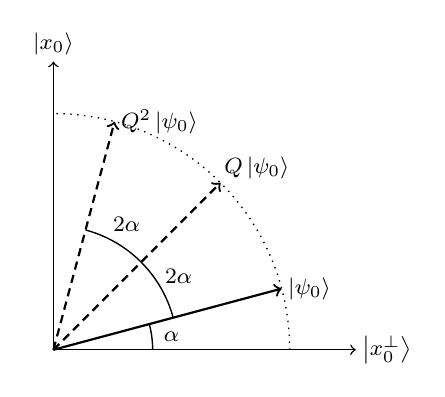
\begin{tikzpicture}[scale=3.0, line width=0.5pt]
	\draw[->] (0,0) -- (1.28,0) node[right, inner sep=2pt] {\footnotesize $\ket{x_0^\perp}$};
	\draw[->] (0,0) -- (0,1.22) node[above, inner sep=2pt] {\footnotesize $\ket{x_0}$};
	\draw[dotted] (1,0) arc[start angle=0, end angle=90, radius=1];
	% psi_0 at angle alpha = 15 deg above the horizontal
	\draw[->, line width=0.8pt] (0,0) -- (0.9659,0.2588) node[right, inner sep=2pt] {\footnotesize $\ket{\psi_0}$};
	% after one iterate: 45 deg
	\draw[->, line width=0.8pt, densely dashed] (0,0) -- (0.7071,0.7071) node[above right, inner sep=1pt] {\footnotesize $Q\ket{\psi_0}$};
	% after two iterates: 75 deg
	\draw[->, line width=0.8pt, densely dashed] (0,0) -- (0.2588,0.9659) node[right, inner sep=2pt] {\footnotesize $Q^2\ket{\psi_0}$};
	% angles
	\draw (0.42,0) arc[start angle=0, end angle=15, radius=0.42];
	\node at (0.50,0.055) {\footnotesize $\alpha$};
	\draw (0.5069,0.1358) arc[start angle=15, end angle=45, radius=0.525];
	\node[fill=white, inner sep=1pt] at (0.53,0.31) {\footnotesize $2\alpha$};
	\draw (0.3712,0.3712) arc[start angle=45, end angle=75, radius=0.525];
	\node[fill=white, inner sep=1pt] at (0.31,0.53) {\footnotesize $2\alpha$};
\end{tikzpicture}
\end{center}

The state starts at angle $\alpha$ above the `all bad' axis, and each application of $Q$ swings it a further $2\alpha$ towards $\ket{x_0}$. When it arrives, a measurement in the computational basis returns $x_0$.

\begin{corollary}
	Let $m$ be the integer nearest to $\dfrac{\pi/2-\alpha}{2\alpha}$, so that
	$$m \approx \frac{\pi}{4}\sqrt N.$$
	Then after $m$ iterations a standard measurement returns $x_0$ with probability $1 - O(1/N)$.
\end{corollary}

\begin{proof}
	After $m$ iterations the state makes an angle $(2m+1)\alpha$ with $\ket{x_0^\perp}$, so the probability of measuring $x_0$ is $\sin^2\left((2m+1)\alpha\right)$. This is maximised by choosing $m$ so that $(2m+1)\alpha$ is as close as possible to $\pi/2$. For large $N$, $\alpha = \arcsin(1/\sqrt N)\approx1/\sqrt N$ is small, so
	$$m\approx\frac{\pi/2}{2\alpha}\approx\frac\pi4\sqrt N,$$
	and rounding to the nearest integer costs us at most $\alpha$ in angle, hence at most $O(\alpha^2) = O(1/N)$ in probability.
\end{proof}

Notice that $m$ does not depend on $x_0$ -- only on $N$. That is essential: we would hardly be able to run the algorithm if the number of steps depended on the answer.

\begin{example}
	Let $N = 4$, so $n = 2$. Here $\sin\alpha = \tfrac12$, so $\alpha = \pi/6$ and each iterate rotates by $2\alpha = \pi/3$. The initial state $\ket{\psi_0} = \ket{++}$ makes an angle $\alpha = \pi/6$ with $\ket{x_0^\perp}$, so after a single iterate it makes an angle $\pi/6+\pi/3 = \pi/2$: it is \emph{exactly} $\ket{x_0}$. One query, and the measurement gives $x_0$ with certainty -- whereas classically we would need up to three. Let us verify directly for $x_0 = 11$. We have $\ket{\psi_0} = \tfrac12(\ket{00}+\ket{01}+\ket{10}+\ket{11})$, so
	$$I_{x_0}\ket{\psi_0} = \tfrac12\left(\ket{00}+\ket{01}+\ket{10}-\ket{11}\right).$$
	Now $I_{\ket{\psi_0}}\ket v = \ket v - 2\ip{\psi_0}{v}\ket{\psi_0}$, and $\ip{\psi_0}{I_{x_0}\psi_0} = \tfrac14(1+1+1-1) = \tfrac12$, so
	$$-I_{\ket{\psi_0}}I_{x_0}\ket{\psi_0} = \ket{\psi_0} - I_{x_0}\ket{\psi_0} = \tfrac12\left(0+0+0+2\ket{11}\right) = \ket{11},$$
	as promised.
\end{example}

\subsection{Multiple Targets and Unknown \texorpdfstring{$r$}{r}}

Now suppose there are $r\geq1$ good items $x_1,\dots,x_r$, with $r$ known. Define
$$I_G = I - 2\sum_{i=1}^r\op{x_i}{x_i},$$
which flips the sign of every good basis state, and is again implemented by one oracle query. Put $Q_G = -I_{\ket{\psi_0}}I_G$, and let
$$\ket{\psi_G} = \frac1{\sqrt r}\sum_{i=1}^r\ket{x_i}, \qquad \ket{\psi_B} = \frac1{\sqrt{N-r}}\sum_{x \text{ bad}}\ket x$$
be the equal superpositions of good and bad items, which are orthonormal. Then
$$\ket{\psi_0} = \sqrt{\frac rN}\ket{\psi_G}+\sqrt{\frac{N-r}{N}}\ket{\psi_B}$$
lies in the plane $\Ps_G = \vecspan\{\ket{\psi_G},\ket{\psi_B}\}$.

\begin{proposition}
	On the plane $\Ps_G$, the operator $Q_G$ acts as a rotation through $2\alpha$, where $\sin\alpha = \ip{\psi_0}{\psi_G} = \sqrt{r/N}$.
\end{proposition}

\begin{proof}
	The only new point is that $I_G$ is not of the form $I_{\ket v}$ for a single vector. But restricted to $\Ps_G$ it is: writing a general element as $a\ket{\psi_G}+b\ket{\psi_B}$, we have
	$$I_G\left(a\ket{\psi_G}+b\ket{\psi_B}\right) = -a\ket{\psi_G}+b\ket{\psi_B},$$
	since $I_G$ negates each good basis vector and fixes each bad one, so on $\Ps_G$ it agrees with $I_{\ket{\psi_G}}$. The proof of the previous theorem now goes through verbatim with $\ket{\psi_G}$ in place of $\ket{x_0}$.
\end{proof}

So the number of iterations is now $m\approx\frac\pi4\sqrt{N/r}$: the more solutions there are, the faster we find one, exactly as one would hope.

The interesting case is when $r$ is \emph{unknown}, which is the realistic one -- for $\mathsf{SAT}$ we have no idea how many satisfying assignments there are. Here we must be careful: running too many iterations is as bad as running too few, since the state rotates \emph{past} $\ket{\psi_G}$ and back down again. The fix is randomisation.

\begin{method}[Grover with Unknown $r$]
	Choose $K$ uniformly at random in $\left(0,\tfrac\pi4\sqrt N\right)$, apply $Q_G$ that many times to $\ket{\psi_0}$, measure, and test the outcome with one further query. Repeat until a good item is found.
\end{method}

\begin{proposition}
	Assuming $r\ll N$, each round of this procedure finds a good item with probability bounded below by an absolute constant, using $O(\sqrt N)$ queries.
\end{proposition}

\begin{proof}[Proof sketch]
	Each iterate rotates by $2\alpha\approx2\sqrt{r/N}$, so applying $K$ of them rotates by a total angle $2K\alpha$, which as $K$ ranges over $(0,\tfrac\pi4\sqrt N)$ ranges over $(0,\tfrac\pi2\sqrt r)$ -- many full turns. The final angle is therefore close to uniform on the circle. If the final state makes an angle within $\pm\pi/4$ of $\ket{\psi_G}$, the probability of measuring a good item is at least $\cos^2(\pi/4) = \tfrac12$. Half of all angles have this property, so the overall success probability per round is about $\tfrac14$. Hence $O(1)$ rounds suffice in expectation, each using $O(\sqrt N)$ queries.
\end{proof}

\subsection{Optimality}

Is $\sqrt N$ the best possible? Yes, and this is one of the few places in the subject where we have a matching lower bound.

\begin{theorem}[BBBV]
	Any quantum algorithm that solves unstructured search on $N$ items with bounded error must make $\Omega(\sqrt N)$ queries. Moreover $\frac\pi4(1-\varepsilon)\sqrt N$ queries do not suffice for any $\varepsilon>0$, so Grover's algorithm is optimal even in its constant.
\end{theorem}

The proof is a `hybrid argument': one shows that a single query can change the state of the computation by only $O(1/\sqrt N)$ in norm on average over the possible locations of the target, so that after $T$ queries the algorithm cannot distinguish the $N$ possible oracles unless $T = \Omega(\sqrt N)$.

The consequence is worth emphasising, because it cuts both ways. On one hand, Grover's algorithm gives a genuine and completely general speedup: any problem for which we know nothing better than brute-force search over $2^n$ candidates -- which includes every $\class{NP}$-complete problem -- can be attacked in time $O(2^{n/2})$ instead of $O(2^n)$. Since $\mathsf{SAT}$ is $\class{NP}$-complete, this applies across the whole of $\class{NP}$.

On the other hand, the lower bound says that this is \emph{all} that generic quantum search can do. To do better one must exploit structure, as Shor does. There is no reason to expect $\class{NP}$-complete problems to have the kind of structure that admits an exponential speedup, and most people do not expect quantum computers to solve them efficiently.

\begin{remark}
	In practice the quadratic speedup is less dramatic than it sounds, since $\sqrt{2^n} = 2^{n/2}$ is still exponential: Grover turns a $128$-bit search into a $64$-bit search. Its main cryptographic consequence is that symmetric key lengths should be doubled, whereas Shor's algorithm destroys RSA and elliptic-curve cryptography outright.
\end{remark}

\section{Mixed States and Density Matrices}

Throughout the course we have described states by vectors, and repeatedly run into situations where that is not quite the right language: a qubit which is `$\ket0$ or $\ket1$ with probability $\tfrac12$ each', or `half of an entangled pair, considered on its own'. In both cases the system has no state vector of its own, yet it certainly has well-defined measurement statistics. The right object is a \vocab{density matrix}, and it lets us say cleanly several things we could previously only say by circumlocution.

\subsection{Density Matrices}

\begin{definition}[Density Matrix]
	Suppose a system is prepared in the state $\ket{\psi_i}$ with probability $p_i$, where $\sum_ip_i=1$. The \vocab{density matrix} of this \vocab{ensemble} is
	$$\rho = \sum_ip_i\op{\psi_i}{\psi_i}.$$
	A state described by a rank-one $\rho = \op\psi\psi$ is called \vocab{pure}; otherwise it is \vocab{mixed}.
\end{definition}

\begin{proposition}
	An operator $\rho$ is the density matrix of some ensemble if and only if it is self-adjoint, positive semi-definite, and has $\Tr\rho = 1$.
\end{proposition}

\begin{proof}
	Each $\op{\psi_i}{\psi_i}$ is self-adjoint and positive semi-definite with trace $\ip{\psi_i}{\psi_i} = 1$, and these properties are preserved by convex combinations. Conversely, given such a $\rho$, the spectral theorem gives $\rho = \sum_i\lambda_i\op{e_i}{e_i}$ with $\lambda_i\geq0$ and $\sum\lambda_i = \Tr\rho = 1$, exhibiting $\rho$ as the density matrix of the ensemble $\{(\lambda_i,\ket{e_i})\}$.
\end{proof}

The Born rule extends immediately: the probability of outcome $j$ in the measurement $\{P_j\}$ is
$$p(j) = \sum_ip_i\mel{\psi_i}{P_j}{\psi_i} = \Tr\left(P_j\rho\right),$$
and unitary evolution acts by $\rho\mapsto U\rho U^\dagger$. Since \emph{all} predictions depend on $\rho$ alone, two ensembles with the same density matrix are physically indistinguishable, however different they look. This is exactly the phenomenon we met in \S3.3.

\begin{example}
	The `yes' ensemble $\{(\tfrac12,\ket0),(\tfrac12,\ket1)\}$ and the `no' ensemble $\{(\tfrac12,\ket+),(\tfrac12,\ket-)\}$ have density matrices
	$$\tfrac12\op00+\tfrac12\op11 = \tfrac12 I, \qquad \tfrac12\op++ + \tfrac12\op-- = \tfrac12I,$$
	which are equal. This \emph{is} the proof that Alice's choice of measurement basis is undetectable by Bob, in one line. The state $\tfrac12I$ is called the \vocab{maximally mixed} state of a qubit.
\end{example}

A useful invariant is the \vocab{purity} $\Tr(\rho^2)$, which satisfies $\tfrac1d\leq\Tr(\rho^2)\leq1$ for a $d$-dimensional system, with equality on the right exactly for pure states and on the left exactly for $\tfrac1dI$. For a qubit one can write
$$\rho = \tfrac12\left(I + \vv{n}\cdot\vec\sigma\right), \qquad \vv n\in\R^3,\ \abs{\vv n}\leq1,$$
where $\vec\sigma = (\sigma_x,\sigma_y,\sigma_z)$; the pure states are those with $\abs{\vv n}=1$. So the density matrices of a qubit fill out the solid \emph{Bloch ball}, with the pure states of \S1.3 forming its surface and the maximally mixed state at the centre.

\subsection{The Reduced Density Matrix}

The other use of density matrices is to describe a subsystem.

\begin{definition}[Partial Trace]
	Let $\rho_{AB}$ be a density matrix on $\Vs_A\otimes\Vs_B$. Its \vocab{partial trace} over $B$ is the operator on $\Vs_A$ defined by
	$$\rho_A = \Tr_B\rho_{AB} = \sum_j\left(I_A\otimes\bra{f_j}\right)\rho_{AB}\left(I_A\otimes\ket{f_j}\right),$$
	where $\{\ket{f_j}\}$ is any orthonormal basis of $\Vs_B$; the result does not depend on the choice.
\end{definition}

\begin{proposition}
	$\rho_A$ is the unique operator on $\Vs_A$ such that $\Tr(M\rho_A) = \Tr\left((M\otimes I)\rho_{AB}\right)$ for every operator $M$ on $\Vs_A$. Consequently $\rho_A$ correctly predicts the statistics of every measurement performed on $A$ alone.
\end{proposition}

\begin{example}
	Take $\ket{\phi^+} = \tfrac1{\sqrt2}(\ket{00}+\ket{11})$, so
	$$\rho_{AB} = \tfrac12\left(\op{00}{00}+\op{00}{11}+\op{11}{00}+\op{11}{11}\right).$$
	Tracing out $B$, the cross terms $\op{00}{11}$ contribute $\ip{1}{0}\op01 = 0$ and similarly for the other, so
	$$\rho_A = \tfrac12\left(\op00+\op11\right) = \tfrac12I.$$
	Alice's half of a Bell pair is maximally mixed: she has \emph{no} information at all. This is the precise sense in which $\ket{\phi^+}$ is maximally entangled, and it is also a one-line proof of the no-signalling principle for this state.
\end{example}

Notice what this says about the relationship between the whole and its parts: $\rho_{AB}$ is pure (we know the joint state exactly) while $\rho_A$ is maximally mixed (we know nothing about the part). Classically this is impossible -- complete knowledge of a pair entails complete knowledge of each member. Entanglement is precisely the failure of that principle.

\begin{proposition}
	A pure state $\ket{\Psi}_{AB}$ is a product state if and only if $\rho_A$ is pure.
\end{proposition}

So the purity $\Tr(\rho_A^2)$ is a quantitative measure of how entangled a pure bipartite state is, running from $1$ (product) down to $1/\dim\Vs_A$ (maximally entangled).

\section{Quantum Error Correction}

The last thing standing between us and a working quantum computer is that quantum systems are appallingly fragile. A qubit interacts with its environment, becomes entangled with it, and -- by the discussion above -- its reduced state becomes mixed: the information leaks away. This process is called \vocab{decoherence}, and without some way of fighting it no quantum computation of any length is possible.

Classically, we fight noise by redundancy: send $000$ instead of $0$, and take a majority vote. Quantumly this looks hopeless for three reasons.

\begin{enumerate}[label=(\roman*)]
	\item We cannot copy an unknown state, by the no-cloning theorem.
	\item We cannot measure the encoded qubits to see whether an error has occurred, since measurement destroys superpositions.
	\item Errors are continuous, not discrete: instead of a bit flip we may get a rotation by a tiny angle $\epsilon$, and there are uncountably many such.
\end{enumerate}

Remarkably, all three objections can be met. We illustrate with the simplest example.

\subsection{The Three-Qubit Bit-Flip Code}

Suppose the only errors that occur are bit flips $X$, acting independently on each qubit with probability $p<\tfrac12$, and suppose at most one qubit is affected. Encode
$$\ket0\longmapsto\ket{0_L} = \ket{000}, \qquad \ket1\longmapsto\ket{1_L}=\ket{111},$$
so that a general qubit $a\ket0+b\ket1$ becomes $a\ket{000}+b\ket{111}$. This is \emph{not} cloning: we have not produced three copies of $a\ket0+b\ket1$, which would be the quite different state $(a\ket0+b\ket1)^{\otimes3}$. Encoding is done with two CNOTs:

\begin{center}
\qcircuit{
	\qwire{0}{0}{8.9}\qwire{-1}{0}{8.9}\qwire{-2}{0}{8.9}
	\qwire{-3.2}{4.1}{8.7}\qwire{-4.2}{4.1}{8.7}
	\qlink{1.0}{0}{-1}\qlink{2.0}{0}{-2}
	\qlink{4.8}{0}{-3.2}\qlink{5.7}{-1}{-3.2}
	\qlink{6.6}{-1}{-4.2}\qlink{7.5}{-2}{-4.2}
	\qtarg{1.0}{-1}\qdot{1.0}{0}
	\qtarg{2.0}{-2}\qdot{2.0}{0}
	\qbig{3.2}{0}{-2}{0.35}{\mathcal{E}}
	\qtarg{4.8}{-3.2}\qdot{4.8}{0}
	\qtarg{5.7}{-3.2}\qdot{5.7}{-1}
	\qtarg{6.6}{-4.2}\qdot{6.6}{-1}
	\qtarg{7.5}{-4.2}\qdot{7.5}{-2}
	\qmeter{8.3}{-3.2}\qmeter{8.3}{-4.2}
	\qlab{0}{0}{\ket{\psi}}\qlab{0}{-1}{\ket{0}}\qlab{0}{-2}{\ket{0}}
	\qlab{4.1}{-3.2}{\ket{0}}\qlab{4.1}{-4.2}{\ket{0}}
	\qrlab{8.7}{-3.2}{s_1}\qrlab{8.7}{-4.2}{s_2}
	\qtext{1.5}{0.85}{\footnotesize encode}
	\qtext{3.2}{0.85}{\footnotesize noise}
	\qtext{6.15}{0.85}{\footnotesize syndrome extraction}
}
\end{center}

The two ancillas measure the parities $s_1 = b_1\oplus b_2$ and $s_2 = b_2\oplus b_3$ of the three data qubits. This is the key move, and it answers objection (ii): we measure a \emph{comparison} of the qubits, not the qubits themselves. Concretely, the measurement is the incomplete projective measurement with the four rank-two projectors
\begin{align*}
	\Pi_{00} &= \op{000}{000}+\op{111}{111}, & \Pi_{10} &= \op{100}{100}+\op{011}{011},\\
	\Pi_{01} &= \op{001}{001}+\op{110}{110}, & \Pi_{11} &= \op{010}{010}+\op{101}{101},
\end{align*}
projecting onto the four two-dimensional subspaces of $(\C^2)^{\otimes3}$ on which the parity pattern is constant.

\begin{proposition}
	If at most one bit flip has occurred, the syndrome $(s_1,s_2)$ identifies which qubit was affected, and the encoded state is undisturbed by the measurement.
\end{proposition}

\begin{proof}
	Write $\mathcal C = \vecspan\{\ket{000},\ket{111}\}$ for the code space. The four error operators $I$, $X_1$, $X_2$, $X_3$ map $\mathcal C$ into the four subspaces
	$$\mathcal C,\quad \vecspan\{\ket{100},\ket{011}\},\quad\vecspan\{\ket{010},\ket{101}\},\quad\vecspan\{\ket{001},\ket{110}\},$$
	which are mutually orthogonal and are exactly the ranges of $\Pi_{00},\Pi_{10},\Pi_{11},\Pi_{01}$ respectively. So the syndrome measurement determines which of the four occurred; and since the corrupted state $X_j(a\ket{000}+b\ket{111})$ lies \emph{entirely} inside one of these subspaces, the corresponding projector acts on it as the identity. The state is therefore not disturbed at all, and in particular the superposition coefficients $a,b$ -- which we do not know and must not learn -- are untouched. Applying $X_j$ to the indicated qubit restores the encoded state.
\end{proof}

That deals with objections (i) and (ii). Objection (iii), the continuum of possible errors, is dealt with by an argument of striking elegance.

\begin{proposition}[Discretisation of Errors]
	Suppose the noise acts on the first qubit by an arbitrary operator, which we may expand in the Pauli basis as $E = c_0I+c_1X+c_2Y+c_3Z$. If the code can correct each of $I,X,Y,Z$ on that qubit, then measuring the syndrome projects the corrupted state onto one of the correctable cases, which we then correct exactly.
\end{proposition}

\begin{proof}[Proof idea]
	Since $\{I,X,Y,Z\}$ spans the space of one-qubit operators, the corrupted state $E_1\ket{\psi_L}$ is a superposition of the four states $\ket{\psi_L}, X_1\ket{\psi_L},Y_1\ket{\psi_L},Z_1\ket{\psi_L}$. If these lie in mutually orthogonal syndrome subspaces, then the syndrome measurement collapses the superposition onto exactly one of them, with the corresponding probability, and we correct it. A continuous error has been \emph{digitised} by the act of measurement.
\end{proof}

(The three-qubit code above corrects $X$ errors only, not $Z$; a $Z$ error would flip the relative sign of $\ket{000}$ and $\ket{111}$ undetected. The conjugate code $\ket{0_L}=\ket{+++}$, $\ket{1_L}=\ket{---}$ corrects $Z$ but not $X$, and concatenating the two gives Shor's nine-qubit code, which corrects an arbitrary error on any one qubit.)

\begin{theorem}[Threshold Theorem]
	There is a constant $p_{\mathrm{th}}>0$ such that, if the physical error rate per gate is below $p_{\mathrm{th}}$, then any quantum circuit of size $T$ can be simulated with error at most $\varepsilon$ by a fault-tolerant circuit of size $O\left(T\,\poly\log(T/\varepsilon)\right)$.
\end{theorem}

This is the reason anyone believes large-scale quantum computing to be possible in principle. It says that error correction is not a losing battle -- once the hardware is good enough, concatenating codes suppresses errors faster than the extra machinery introduces them, and the overhead is only polylogarithmic.

\section{Closing Remarks}

Let us take stock of what quantum mechanics has bought us.

\emph{Impossibility.} Non-orthogonal states cannot be reliably distinguished (\S2.3); unknown states cannot be cloned (\S3.2); measurement at a distance cannot signal (\S3.4). These are not engineering limitations but theorems, and each follows from linearity and unitarity in a few lines.

\emph{New protocols.} Entanglement lets us send two classical bits down one qubit (\S6) and one qubit down two classical bits (\S7), and lets us distribute cryptographic keys whose security rests on physics rather than on computational assumptions (\S8). None of these is possible classically.

\emph{New algorithms.} Superposition, phase kickback and interference give exact one-query solutions to Deutsch and Deutsch--Jozsa (\S10), an exponential bounded-error separation in Simon's problem (\S10.3), polynomial-time factoring via period-finding and the quantum Fourier transform (\S12), and a provably optimal quadratic speedup for unstructured search (\S13).

\emph{And what quantum mechanics does not buy us.} A quantum computer computes exactly the same functions as a classical one; the difference is only in efficiency, and even there we have no \emph{proof} of a separation, only very strong evidence. Grover's bound tells us that generic search cannot do better than quadratic, so $\class{NP}$-complete problems are almost certainly not going to fall. And every protocol we have seen respects relativistic causality: nothing here travels faster than a classical message.

Perhaps the deepest lesson is Landauer's: \emph{information is physical}. The theory of computation is not a branch of pure mathematics floating free of the world, but a description of what physical systems can be made to do. Change the physics and you change the theory. It is a striking thought that the answer to `what is efficiently computable?' should depend on the correct theory of nature -- and a slightly unsettling one that we do not yet know the final answer to either question.
\end{document}
